% Options for packages loaded elsewhere
\PassOptionsToPackage{unicode}{hyperref}
\PassOptionsToPackage{hyphens}{url}
\PassOptionsToPackage{dvipsnames,svgnames,x11names}{xcolor}
%
\documentclass[
  letterpaper,
  DIV=11,
  numbers=noendperiod]{scrreprt}

\usepackage{amsmath,amssymb}
\usepackage{iftex}
\ifPDFTeX
  \usepackage[T1]{fontenc}
  \usepackage[utf8]{inputenc}
  \usepackage{textcomp} % provide euro and other symbols
\else % if luatex or xetex
  \usepackage{unicode-math}
  \defaultfontfeatures{Scale=MatchLowercase}
  \defaultfontfeatures[\rmfamily]{Ligatures=TeX,Scale=1}
\fi
\usepackage{lmodern}
\ifPDFTeX\else  
    % xetex/luatex font selection
\fi
% Use upquote if available, for straight quotes in verbatim environments
\IfFileExists{upquote.sty}{\usepackage{upquote}}{}
\IfFileExists{microtype.sty}{% use microtype if available
  \usepackage[]{microtype}
  \UseMicrotypeSet[protrusion]{basicmath} % disable protrusion for tt fonts
}{}
\makeatletter
\@ifundefined{KOMAClassName}{% if non-KOMA class
  \IfFileExists{parskip.sty}{%
    \usepackage{parskip}
  }{% else
    \setlength{\parindent}{0pt}
    \setlength{\parskip}{6pt plus 2pt minus 1pt}}
}{% if KOMA class
  \KOMAoptions{parskip=half}}
\makeatother
\usepackage{xcolor}
\setlength{\emergencystretch}{3em} % prevent overfull lines
\setcounter{secnumdepth}{5}
% Make \paragraph and \subparagraph free-standing
\ifx\paragraph\undefined\else
  \let\oldparagraph\paragraph
  \renewcommand{\paragraph}[1]{\oldparagraph{#1}\mbox{}}
\fi
\ifx\subparagraph\undefined\else
  \let\oldsubparagraph\subparagraph
  \renewcommand{\subparagraph}[1]{\oldsubparagraph{#1}\mbox{}}
\fi

\usepackage{color}
\usepackage{fancyvrb}
\newcommand{\VerbBar}{|}
\newcommand{\VERB}{\Verb[commandchars=\\\{\}]}
\DefineVerbatimEnvironment{Highlighting}{Verbatim}{commandchars=\\\{\}}
% Add ',fontsize=\small' for more characters per line
\usepackage{framed}
\definecolor{shadecolor}{RGB}{241,243,245}
\newenvironment{Shaded}{\begin{snugshade}}{\end{snugshade}}
\newcommand{\AlertTok}[1]{\textcolor[rgb]{0.68,0.00,0.00}{#1}}
\newcommand{\AnnotationTok}[1]{\textcolor[rgb]{0.37,0.37,0.37}{#1}}
\newcommand{\AttributeTok}[1]{\textcolor[rgb]{0.40,0.45,0.13}{#1}}
\newcommand{\BaseNTok}[1]{\textcolor[rgb]{0.68,0.00,0.00}{#1}}
\newcommand{\BuiltInTok}[1]{\textcolor[rgb]{0.00,0.23,0.31}{#1}}
\newcommand{\CharTok}[1]{\textcolor[rgb]{0.13,0.47,0.30}{#1}}
\newcommand{\CommentTok}[1]{\textcolor[rgb]{0.37,0.37,0.37}{#1}}
\newcommand{\CommentVarTok}[1]{\textcolor[rgb]{0.37,0.37,0.37}{\textit{#1}}}
\newcommand{\ConstantTok}[1]{\textcolor[rgb]{0.56,0.35,0.01}{#1}}
\newcommand{\ControlFlowTok}[1]{\textcolor[rgb]{0.00,0.23,0.31}{#1}}
\newcommand{\DataTypeTok}[1]{\textcolor[rgb]{0.68,0.00,0.00}{#1}}
\newcommand{\DecValTok}[1]{\textcolor[rgb]{0.68,0.00,0.00}{#1}}
\newcommand{\DocumentationTok}[1]{\textcolor[rgb]{0.37,0.37,0.37}{\textit{#1}}}
\newcommand{\ErrorTok}[1]{\textcolor[rgb]{0.68,0.00,0.00}{#1}}
\newcommand{\ExtensionTok}[1]{\textcolor[rgb]{0.00,0.23,0.31}{#1}}
\newcommand{\FloatTok}[1]{\textcolor[rgb]{0.68,0.00,0.00}{#1}}
\newcommand{\FunctionTok}[1]{\textcolor[rgb]{0.28,0.35,0.67}{#1}}
\newcommand{\ImportTok}[1]{\textcolor[rgb]{0.00,0.46,0.62}{#1}}
\newcommand{\InformationTok}[1]{\textcolor[rgb]{0.37,0.37,0.37}{#1}}
\newcommand{\KeywordTok}[1]{\textcolor[rgb]{0.00,0.23,0.31}{#1}}
\newcommand{\NormalTok}[1]{\textcolor[rgb]{0.00,0.23,0.31}{#1}}
\newcommand{\OperatorTok}[1]{\textcolor[rgb]{0.37,0.37,0.37}{#1}}
\newcommand{\OtherTok}[1]{\textcolor[rgb]{0.00,0.23,0.31}{#1}}
\newcommand{\PreprocessorTok}[1]{\textcolor[rgb]{0.68,0.00,0.00}{#1}}
\newcommand{\RegionMarkerTok}[1]{\textcolor[rgb]{0.00,0.23,0.31}{#1}}
\newcommand{\SpecialCharTok}[1]{\textcolor[rgb]{0.37,0.37,0.37}{#1}}
\newcommand{\SpecialStringTok}[1]{\textcolor[rgb]{0.13,0.47,0.30}{#1}}
\newcommand{\StringTok}[1]{\textcolor[rgb]{0.13,0.47,0.30}{#1}}
\newcommand{\VariableTok}[1]{\textcolor[rgb]{0.07,0.07,0.07}{#1}}
\newcommand{\VerbatimStringTok}[1]{\textcolor[rgb]{0.13,0.47,0.30}{#1}}
\newcommand{\WarningTok}[1]{\textcolor[rgb]{0.37,0.37,0.37}{\textit{#1}}}

\providecommand{\tightlist}{%
  \setlength{\itemsep}{0pt}\setlength{\parskip}{0pt}}\usepackage{longtable,booktabs,array}
\usepackage{calc} % for calculating minipage widths
% Correct order of tables after \paragraph or \subparagraph
\usepackage{etoolbox}
\makeatletter
\patchcmd\longtable{\par}{\if@noskipsec\mbox{}\fi\par}{}{}
\makeatother
% Allow footnotes in longtable head/foot
\IfFileExists{footnotehyper.sty}{\usepackage{footnotehyper}}{\usepackage{footnote}}
\makesavenoteenv{longtable}
\usepackage{graphicx}
\makeatletter
\def\maxwidth{\ifdim\Gin@nat@width>\linewidth\linewidth\else\Gin@nat@width\fi}
\def\maxheight{\ifdim\Gin@nat@height>\textheight\textheight\else\Gin@nat@height\fi}
\makeatother
% Scale images if necessary, so that they will not overflow the page
% margins by default, and it is still possible to overwrite the defaults
% using explicit options in \includegraphics[width, height, ...]{}
\setkeys{Gin}{width=\maxwidth,height=\maxheight,keepaspectratio}
% Set default figure placement to htbp
\makeatletter
\def\fps@figure{htbp}
\makeatother
\newlength{\cslhangindent}
\setlength{\cslhangindent}{1.5em}
\newlength{\csllabelwidth}
\setlength{\csllabelwidth}{3em}
\newlength{\cslentryspacingunit} % times entry-spacing
\setlength{\cslentryspacingunit}{\parskip}
\newenvironment{CSLReferences}[2] % #1 hanging-ident, #2 entry spacing
 {% don't indent paragraphs
  \setlength{\parindent}{0pt}
  % turn on hanging indent if param 1 is 1
  \ifodd #1
  \let\oldpar\par
  \def\par{\hangindent=\cslhangindent\oldpar}
  \fi
  % set entry spacing
  \setlength{\parskip}{#2\cslentryspacingunit}
 }%
 {}
\usepackage{calc}
\newcommand{\CSLBlock}[1]{#1\hfill\break}
\newcommand{\CSLLeftMargin}[1]{\parbox[t]{\csllabelwidth}{#1}}
\newcommand{\CSLRightInline}[1]{\parbox[t]{\linewidth - \csllabelwidth}{#1}\break}
\newcommand{\CSLIndent}[1]{\hspace{\cslhangindent}#1}

\KOMAoption{captions}{tableheading}
\makeatletter
\makeatother
\makeatletter
\@ifpackageloaded{bookmark}{}{\usepackage{bookmark}}
\makeatother
\makeatletter
\@ifpackageloaded{caption}{}{\usepackage{caption}}
\AtBeginDocument{%
\ifdefined\contentsname
  \renewcommand*\contentsname{Table of contents}
\else
  \newcommand\contentsname{Table of contents}
\fi
\ifdefined\listfigurename
  \renewcommand*\listfigurename{List of Figures}
\else
  \newcommand\listfigurename{List of Figures}
\fi
\ifdefined\listtablename
  \renewcommand*\listtablename{List of Tables}
\else
  \newcommand\listtablename{List of Tables}
\fi
\ifdefined\figurename
  \renewcommand*\figurename{Figure}
\else
  \newcommand\figurename{Figure}
\fi
\ifdefined\tablename
  \renewcommand*\tablename{Table}
\else
  \newcommand\tablename{Table}
\fi
}
\@ifpackageloaded{float}{}{\usepackage{float}}
\floatstyle{ruled}
\@ifundefined{c@chapter}{\newfloat{codelisting}{h}{lop}}{\newfloat{codelisting}{h}{lop}[chapter]}
\floatname{codelisting}{Listing}
\newcommand*\listoflistings{\listof{codelisting}{List of Listings}}
\usepackage{amsthm}
\theoremstyle{plain}
\newtheorem{theorem}{Theorem}[chapter]
\theoremstyle{definition}
\newtheorem{definition}{Definition}[chapter]
\theoremstyle{plain}
\newtheorem{lemma}{Lemma}[chapter]
\theoremstyle{remark}
\AtBeginDocument{\renewcommand*{\proofname}{Proof}}
\newtheorem*{remark}{Remark}
\newtheorem*{solution}{Solution}
\makeatother
\makeatletter
\@ifpackageloaded{caption}{}{\usepackage{caption}}
\@ifpackageloaded{subcaption}{}{\usepackage{subcaption}}
\makeatother
\makeatletter
\@ifpackageloaded{tcolorbox}{}{\usepackage[skins,breakable]{tcolorbox}}
\makeatother
\makeatletter
\@ifundefined{shadecolor}{\definecolor{shadecolor}{rgb}{.97, .97, .97}}
\makeatother
\makeatletter
\makeatother
\makeatletter
\makeatother
\ifLuaTeX
  \usepackage{selnolig}  % disable illegal ligatures
\fi
\IfFileExists{bookmark.sty}{\usepackage{bookmark}}{\usepackage{hyperref}}
\IfFileExists{xurl.sty}{\usepackage{xurl}}{} % add URL line breaks if available
\urlstyle{same} % disable monospaced font for URLs
\hypersetup{
  pdftitle={MA42002},
  pdfauthor={Philip Murray},
  colorlinks=true,
  linkcolor={blue},
  filecolor={Maroon},
  citecolor={Blue},
  urlcolor={Blue},
  pdfcreator={LaTeX via pandoc}}

\title{MA42002}
\author{Philip Murray}
\date{2023-12-22}

\begin{document}
\maketitle
\ifdefined\Shaded\renewenvironment{Shaded}{\begin{tcolorbox}[breakable, borderline west={3pt}{0pt}{shadecolor}, sharp corners, interior hidden, boxrule=0pt, enhanced, frame hidden]}{\end{tcolorbox}}\fi

\renewcommand*\contentsname{Table of contents}
{
\hypersetup{linkcolor=}
\setcounter{tocdepth}{2}
\tableofcontents
}
\bookmarksetup{startatroot}

\hypertarget{introduction}{%
\chapter*{Introduction}\label{introduction}}
\addcontentsline{toc}{chapter}{Introduction}

\markboth{Introduction}{Introduction}

Welcome to MA42002 Mathematical Biology II.

My name is Philip Murray and I am the module lead.

\hypertarget{how-to-contact-me}{%
\section*{How to contact me?}\label{how-to-contact-me}}
\addcontentsline{toc}{section}{How to contact me?}

\markright{How to contact me?}

\begin{itemize}
\tightlist
\item
  email: pmurray@dundee.ac.uk
\item
  office: G11, Fulton Building
\end{itemize}

\hypertarget{lecture-notes}{%
\section*{Lecture notes}\label{lecture-notes}}
\addcontentsline{toc}{section}{Lecture notes}

\markright{Lecture notes}

You can find lecture notes for the module on this page. If you would
like a pdf this can be easily generated by clikcing on the pdf link on
the top left of the webpages. I will occasionally edit/update the notes
we proceed through lectures. If you spot any errors, typos or omissions
please let me know.

\hypertarget{reading}{%
\section*{Reading}\label{reading}}
\addcontentsline{toc}{section}{Reading}

\markright{Reading}

Mathematical Biology II, James Dickson Murray (2003)

\hypertarget{python-codes}{%
\section*{Python codes}\label{python-codes}}
\addcontentsline{toc}{section}{Python codes}

\markright{Python codes}

I have provided Python codes for most of the figures in the notes (you
can unfold code section by clicking `Code'). Many of you have taken the
Introduction to Programming module at Level 2 and have therefore some
experience using Python. I strongly encourage you to use the provided
codes as a tool to play around with numerical solutions of the various
models that we will be working on. The codes should run as standalone
Python codes.

\bookmarksetup{startatroot}

\hypertarget{conservation-equations}{%
\chapter{Conservation equations}\label{conservation-equations}}

\hypertarget{sec-conservation}{%
\section{Introduction}\label{sec-conservation}}

Many biological systems are spatio-temporal, i.e.~concentrations of
biochemicals, densities of cells etc. depend on spatial position as well
time. To describe such cases we must \textbf{relax} a major assumption
that was made in Mathematical Biology I (MA32009): spatial homogeneity.
We now models biological system using partial differential equations.

A conservation equation is the most fundamental statement through which
changes in the distribution of the density (or concentration,
temperature) is described. \[
\begin{pmatrix}
\text{rate of change}\\
\text{ in the population density} 
\end{pmatrix}
= \begin{pmatrix}
\text{spatial movement}
\end{pmatrix}
+ 
 \begin{pmatrix}
 \text{birth, growth, death},\\
 \text{production or degradation}\\
  \text{due to chemical reactions} 
\end{pmatrix}
\]

\hypertarget{notation}{%
\subsection{Notation}\label{notation}}

We will consider \(x \in \mathbb R^n\), \(t \in [0, \infty)\) and
functions \(c: \mathbb R^n \times [0, \infty) \to \mathbb R\), where
\(n=1,2,3\). For example:

\begin{itemize}
\tightlist
\item
  \(c(x,t)\) - the density of a population {[}number per volume{]} at
  position \(x\) and time \(t\) (at \((x,t)\))
\item
  \(c(x,t)\) - the concentration of a substance (chemicals, particles)
  {[}mass per volume{]} at position \(x\) and time \(t\) (at \((x,t)\))
\item
  \(c(x,t)\) - the temperature at \((x,t)\).
\end{itemize}

\hypertarget{spatially-homogeneous-models}{%
\section{Spatially homogeneous
models}\label{spatially-homogeneous-models}}

In this section, we neglect spatial movement and consider examples of
growth/death and chemical reactions (i.e.~revision from MA32009).

\hypertarget{population-dynamics}{%
\subsection{Population dynamics}\label{population-dynamics}}

\hypertarget{modelling-the-growth-of-bacteria-in-a-petri-dish-flask-containing-nutrient-medium}{%
\subsubsection{Modelling the growth of bacteria in a petri dish (flask)
containing nutrient
medium}\label{modelling-the-growth-of-bacteria-in-a-petri-dish-flask-containing-nutrient-medium}}

As an example let's consider a population of bacteria growing in a
bounded domain (e.g.~a petri dish).

Bacteria reproduce by undergoing successive cell divisions.

Let \(N(t)\) represent bacterial density at time \(t\) (i.e.~number of
cells per volume).

Let \(K\) represent the \emph{per capita} rate of reproduction. Over a
period of time, \(\Delta t\), \(K N(t) \Delta t\) cells will be added.
Hence \begin{equation}\protect\hypertarget{eq-n_1}{}{ 
\begin{aligned}
N(t+\Delta t) &=  \quad N(t)   + \quad  K N(t) \Delta t.
\end{aligned}
}\label{eq-n_1}\end{equation} Assuming that \(N\) is differentiable,
dividing Equation~\ref{eq-n_1} by \(\Delta t\) and taking the limit as
\(\Delta t \to 0\) \begin{equation}\protect\hypertarget{eq-n_2}{}{
 \frac{dN}{dt} = K N 
}\label{eq-n_2}\end{equation}

Depending on the biological context, the growth rate \(K\) may take
several forms e.g.~

\begin{itemize}
\tightlist
\item
  \(K = \textrm{constant}\)
\item
  \(K = K(t)\) \qquad  time-dependent
\item
  \(K= K(N(t))\) \qquad depends on bacterial density
\item
  \(K= K(c(t)):= \kappa c(t), \;\; (\text{with} \;\; \kappa >0 \;\; \text{a constant}\)),
  which depends on the nutrient concentration \(c(t)\) at time \(t\)
  i.e.~\(K\) depends on the available resources.
\end{itemize}

\hypertarget{logistic-growth-via-depleting-nutrient-source}{%
\subsubsection{Logistic growth via depleting nutrient
source}\label{logistic-growth-via-depleting-nutrient-source}}

Suppose that the population growth rate depends on nutient availability.
Suppose also that nutrient levels are depleted by population growth.

Let \(c(t)\) represent the nutrient concentration at time, \(t\). Bawed
on the above assumptions we derive
\begin{equation}\protect\hypertarget{eq-c_1}{}{
\begin{aligned}
\frac{dN}{dt} &= K(c) N = \kappa cN,  \\
 \frac{ dc}{dt} &= - \alpha \frac{dN}{dt} = - \alpha   \kappa c N,  
 \end{aligned}
}\label{eq-c_1}\end{equation} where \(\kappa\) and \(\alpha\)
\(\in \Re\). Consider the initial conditions \[
 N(0) = N_0 \quad \textrm{and}  \quad  c(0)= c_0.
\]

Noting the conserved quantity \[
\frac{dN}{dt}+\frac{dc}{dt}=0,
\] integration yields \begin{equation}\protect\hypertarget{eq-sol_c}{}{
c(t)  = - \alpha N(t) + c(0)+ \alpha N(0) = - \alpha N(t) + \beta,
}\label{eq-sol_c}\end{equation} where \(\beta=c_0 +\alpha N_0\). Using
Equation~\ref{eq-sol_c} in Equation~\ref{eq-c_1} we obtain the
\emph{logistic growth} equation
\begin{equation}\protect\hypertarget{eq-n_4}{}{
\frac{dN}{dt} = \kappa ( \beta- \alpha N)  N, \qquad  N(0)= N_0\quad  
}\label{eq-n_4}\end{equation} Here we have
\(K=K(N) = \kappa (\beta - \alpha N)\).

The last equation can be rewritten as
\begin{equation}\protect\hypertarget{eq-n_5}{}{  
\frac{dN}{dt} = \rho  N \,  (1 - \frac N B)  \qquad \quad N(0)= N_0, 
}\label{eq-n_5}\end{equation} where \(\rho = \kappa \beta\) is the
\textbf{intrinsic growth rate} and \(B = \frac \beta \alpha\) is the
\textbf{carrying capacity}. The solution of Equation~\ref{eq-n_5} is
given by \[
N(t)= \frac{ N_0 K} { N_0 + (B-N_0) e^{-\rho t}} \; .
\]

\hypertarget{deathdecay}{%
\subsubsection{Death/decay}\label{deathdecay}}

In addition to growth, we may assume that cells die at rate \(d\) and
the simple growth Equation~\ref{eq-n_2} can be generalised to \[
\frac{dN}{dt} = KN - d N, 
\] where \(d\) is the mortality (death) rate.

\hypertarget{competition}{%
\subsubsection{Competition}\label{competition}}

The fact that individuals compete for food, habitat (i.e.~space) or any
limited resources, means that an increase in the net mortality of the
population may be observed under crowded conditions. Hence we could
obtain \[
\frac{dN}{dt} = KN - d_1 N^2 , 
\] where \(d=d_1N\) is the mortality (death) rate and is proportional to
the population density.

\hypertarget{sir-model}{%
\subsection{SIR Model}\label{sir-model}}

Consider a model of infectious diease in which a population is slit into
three compartments:

\begin{itemize}
\tightlist
\item
  susceptible
\item
  infected
\item
  recoveered
\end{itemize}

Suppse that interaction between suspectible and infected results in
infection of susceptible. Suppose also that infected people only remain
infectious for a limited time.

Let \(S(t)\), \(I(t)\) and \(R(t)\) represent the population densities
of susceptible, infected and recoveered populations, respectively.

Consider the governing ODE

\[
\begin{aligned}
\frac{d S}{ dt} &= -rIS, \\
\frac{d I}{ dt} &= rIS - aI, \\
\frac{d R}{ dt} &= aI,
\end{aligned}
\] where \(r\) is the infection rate and \(a\) is the recovery rate.

\hypertarget{activator-inhibitor-kinetics}{%
\subsection{Activator inhibitor
kinetics}\label{activator-inhibitor-kinetics}}

Consider a pair of interacting biochemical species, A and B. Suppose
that both A and B are produced at a constant rate and that A underfgoes
linear degradation. Suppose also that A and B interact \[
2A+B \rightarrow A.
\]

Applying the law of mass action we obtain the ODEs \[
\begin{aligned}
\frac{d A}{ dt} &= k_1 - k_2 A + k_3 A^2 B,  \\
\frac{d B}{ dt} &= k_4 - k_3 A^2 B,
\end{aligned}
\] where \(k_1\) and \(k_4\) are production rates, \(k_2\) is a
degradation rate and \(k_3\) is the reaction rate for the A and B
interaction.

\hypertarget{spatial-movement}{%
\section{Spatial movement}\label{spatial-movement}}

Consider a spatial domain \(V\). A conservation equation can be written
either in terms of the mass or number of particles of a species as
follows:

\[
\begin{pmatrix}
\text{rate of change of}\\
\text{number of particles} \\
\text{per unit time } 
\end{pmatrix}
= \begin{pmatrix}
\text{rate of entry of}\\
\text{particles into $V$}\\
\text{per unit time}
\end{pmatrix}
- \begin{pmatrix}
\text{rate of exit of }\\
\text{particles from $V$}\\
\text{per unit time}
\end{pmatrix}
+ 
 \begin{pmatrix}
 \text{rate of degradation}\\
 \text{or creation of particles }\\
  \text{in $V$ per unit time} 
\end{pmatrix}
\]

\hypertarget{one-dimensional-conservation-equations}{%
\subsection{One-dimensional conservation
equations}\label{one-dimensional-conservation-equations}}

Assume

\begin{itemize}
\tightlist
\item
  motion takes place in a one-dimensional domain (e.g.~a long very thin
  tube)
\item
  the tube has a constant cross-section area
\end{itemize}

Let \(x\) be the distance along the tube relative to an origin. We shall
consider the interval \((x+\Delta x, t)\), for some \(\Delta x >0\), and
a domain \(V= (x, x+ \Delta x) \times S\), where \(S\) is the
cross-section of the tube with the constant area \(A=|S|\).

\begin{itemize}
\item
  \(c(x,t)\) - concentration of particles (number of particles per unit
  volume) at time, \(t\), and position, \(x\)
\item
  \(J(x,t)\) - flux of particles per unit time and unit area (number of
  particles crossing a unit area in the positive \(x\)-direction per
  unit time)
\item
  \(f(x,t ,c(x,t))\) - source/sink (number of particles created or
  destroyed per unit volume and unit time)
\end{itemize}

We consider \(S\) to be very small and \(c(x,t)\) is assumed to be
constant in \(S\) (independent of \(y\) and \(z\)). We also assume that
\(c\) is continuously differentiable with respect to \(t\).

The volume of \(V\) is \(A \Delta x\) and number of particles is given
by \[
\int_x^{x+\Delta x} c(\tilde x, t) \,  d \tilde x A.
\]

Then the conservation equation for the number of particles in the volume
\(V\) is given by \begin{equation}\protect\hypertarget{eq-concerv_01}{}{
\frac{\partial}{\partial t} \int_x^{x+\Delta x} c(\tilde x, t) A d\tilde x = J(x,t) \, A  - J(x+\Delta x,t) \, A +\int_x^{x + \Delta x}  f(\tilde x, t, c(\tilde x, t))\,  A \, d \tilde x.
}\label{eq-concerv_01}\end{equation}

i.e.~the flux that changes the total population in \(V\) is that
entering through the cross-section at \(x\) and leaving through the
cross-section at \(x+\Delta x\) (it is assumed that there no flux
through the external surface of the tube). Assuming \(c\) and \(f\) to
be sufficiently smooth (continuous in \(x\)) and applying The Mean Value
Theorem in Equation~\ref{eq-concerv_01}, we obtain
\begin{equation}\protect\hypertarget{eq-concerv_1}{}{
\frac{\partial}{\partial t} c(\xi, t) A \Delta x = J(x,t) \, A  - J(x+\Delta x,t) \, A +  f(\eta,t,c(\eta, t))\,  A \Delta x, \qquad \xi, \eta \in (x, x+ \Delta x).
}\label{eq-concerv_1}\end{equation}

Dividing Equation~\ref{eq-concerv_01} by \(A \, \Delta x\) yields
\begin{equation}\protect\hypertarget{eq-concerv_2}{}{
\frac{\partial}{\partial t} c(\xi, t)  = - \frac  {J(x+\Delta x,t ) - J(x,t)} { \Delta x} + f(\eta,t,c(\eta, t)), \qquad \xi, \eta \in (x, x+ \Delta x).
}\label{eq-concerv_2}\end{equation} Assuming that \(J\) is
differentiable with respect to \(x\) and taking the limit as
\(\Delta x \to 0\) (and using the definition of partial derivatives) we
obtain a one-dimensional conservation (balance) equation:
\begin{equation}\protect\hypertarget{eq-concerv_3}{}{
\frac{\partial}{\partial t} c(x,t)  = - \frac  {\partial} { \partial x} J(x,t) + f(x,t ,c(x,t)).
}\label{eq-concerv_3}\end{equation}

\hypertarget{conservation-equations-in-mathbb-rn}{%
\subsection{\texorpdfstring{Conservation equations in
\(\mathbb R^n\)}{Conservation equations in \textbackslash mathbb R\^{}n}}\label{conservation-equations-in-mathbb-rn}}

Let \(V \subset \mathbb R^n\) be an arbitrary bounded domain
(i.e.~satisfying the conditions of the divergence theorem) and let \(S\)
be the surface enclosing \(V\), i.e \(S = \partial V\).

\begin{itemize}
\tightlist
\item
  \(c(x,t)\) -- concentration of particles at \(x\in V\) and \(t>0\)
  (number of particles per unit volume)
\item
  \(J(x,t)\) -- flux vector of particles across \(V\) (number of
  particles per unit area and per unit time entering or leaving through
  \(S\) (the boundary of \(V\)).
\item
  \(f(x,t ,c(x,t))\) - source/sink term (number of particles created or
  destroyed per unit volume and per unit time)
\end{itemize}

Then the conservation equation reads \[
\frac{\partial}{\partial t} \int_V c(x,t) \, dx = - \int_{S} J(x,t) \cdot {\mathbf{n}} \, d\sigma + \int_V f(x,t ,c), 
\] where \(\mathbf{n}\) is the outward normal vector to \(S\). The
normal component of the flux \(J\) on \(S\) leads to a change of number
of particles (of mass) in \(V\). Applying the divergence theorem, i.e.
\[
\int_S J \cdot {\mathbf{n}} \, d\sigma = \int_V \text{ div} J \, dx,
\] and using the fact that \(V\) is independent of time \(t\) we obtain
\[
 \int_V \Big(\frac{\partial}{\partial t} c(x,t) + \nabla \cdot  J(x,t) -  f(x,t ,c)\Big) dx.
\] Since \(V\) can be chosen arbitrary we get the conservation equation
in \(\mathbb R^n\) (or a subdomain \(\Omega \subset \mathbb R^n\))

\begin{equation}\protect\hypertarget{eq-conservation_3D}{}{
\frac{\partial}{\partial t} c(x,t) =  - \nabla \cdot  J(x,t)+  f(x,t ,c), \quad x\in \mathbb R^n \,  (\text{or } x \in \Omega), \quad t >0. 
}\label{eq-conservation_3D}\end{equation}

\hypertarget{types-of-flux-terms}{%
\subsection{Types of flux terms}\label{types-of-flux-terms}}

\begin{itemize}
\item
  Fickian Diffusion

  Diffusion is an important and `'metabolically cheap'' transport
  mechanism in biological systems. It can be also viewed as the random
  motion of individual molecules.

  \begin{equation}\protect\hypertarget{eq-diffusion}{}{
  {\mathbf{J}} = - D\nabla c,
  }\label{eq-diffusion}\end{equation} where \(D\) is the diffusion
  coefficient. \(D\) depends on the size of the particles, the type of
  solvent, the temperature, \ldots.

  Then applying Equation~\ref{eq-diffusion} in
  Equation~\ref{eq-conservation_3D} we obtain reaction-diffusion
  equation \begin{equation}\protect\hypertarget{eq-react-diff}{}{
  \frac{\partial}{\partial t} c =  - \nabla\cdot ( - D \nabla c(x,t))+  f(x,t ,c) = \nabla \cdot ( D \nabla c) + f(x,t ,c),
  \quad x\in \mathbb R^n, \,  \, t >0.
  }\label{eq-react-diff}\end{equation}

  If \(D\) is a constant we can write \[
  \frac{\partial}{\partial t} c(x,t) =  D \Delta c(x,t) + f(x,t ,c),
  \quad x\in \mathbb R^n \,  (\text{or } x \in \Omega), \quad t >0, 
  \]\\
  where \[
  \Delta c = \sum\limits_{j=1}^n \dfrac{\partial^2 c}{\partial x_j^2}.
  \]
\item
  Nonlinear diffusion \[
  D = D(c) , \qquad \text{ e.g. }\,   D(c)= D_0 c^m, \quad D_0 >0, 
  \] and \begin{equation}\protect\hypertarget{eq-diff_nonlin}{}{
    \frac{\partial}{\partial t} c = D_0 \nabla\cdot (c^m \nabla c) + f(x,t ,c),
  \quad x\in \mathbb R^n,  \quad t >0.
  }\label{eq-diff_nonlin}\end{equation}
\item
  Convection or Advection \[ 
  J = \textbf{v} c,
  \] where \(\textbf{v}\) is a velocity vector. Hence
  \begin{equation}\protect\hypertarget{eq-convection}{}{
  \frac{\partial}{\partial t} c(x,t) = - \nabla\cdot (\textbf{v}(x,t) c(x,t))  + f(x,t ,c),
  \quad x\in \mathbb R^n,   \quad t >0. 
  }\label{eq-convection}\end{equation}

  If \(\textbf{v}\) is constant or \(\nabla \cdot \textbf{v} = 0\), then
  \[
  \frac{\partial}{\partial t} c = - \textbf{v} \nabla c  + f(x,t ,c)
  \quad x\in \mathbb R^n, \,  \quad t >0.
  \]
\item
  Taxis - directed movement in response to an external chemical or
  physical signal.

  \begin{itemize}
  \tightlist
  \item
    chemotaxis - movement directed by a chemical gradient
  \item
    haptotaxis - movement directed by a gradient in density, adhesion
  \end{itemize}

  In the presence of some chemoattractant \(a(x,t)\) we have \[
    {\mathbf{J}} = \chi(a) c \nabla a,  
    \] where \(\chi(a)\) is a `model-specific' function of \(a\)
  defining the sensitivity to the signal, and the conservation equation
  reads \begin{equation}\protect\hypertarget{eq-taxis}{}{
    \frac{\partial}{\partial t} c(x,t) = -\nabla \cdot (\chi(a) c(x,t) \nabla a )  + f(x,t ,c),
    \quad x\in \mathbb R^n \,  \quad t >0. 
    }\label{eq-taxis}\end{equation}
\end{itemize}

\hypertarget{boundary-conditions-b.c.}{%
\subsection{Boundary conditions (B.C.)}\label{boundary-conditions-b.c.}}

\begin{itemize}
\tightlist
\item
  Infinite domain (e.g.~\((-\infty, \infty)\), \(\mathbb R^2\),
  \(\mathbb R^3\) ):
\end{itemize}

the density is not influenced by the boundary \[
c(x,t) \to 0 \qquad \text{ as } \qquad \|x\| \to \infty \quad  \text{decay at infinity}
\]

\begin{itemize}
\tightlist
\item
  Periodic B.C.
\end{itemize}

\(L\)-periodic function: \(c(x,t) = c(x,t +L)\) for any \(x\) in the
domain

Consider a domain \((0,L)\). \[
c(t,0) = c(t,L) \qquad  \text{ periodic boundary conditions}
\]

\begin{itemize}
\tightlist
\item
  Dirichlet B.C.
\end{itemize}

density (concentration) is fixed at the boundary

In the \(1\)-dim domain \((0,L)\) \[
c(t,0) = c_1, \quad  c(t,L) = c_2
\] can consider two reservoirs placed at the ends of the domain, that
are held at constant densities (concentrations) \(c_1\) and \(c_2\),
respectively.

For a domain \(\Omega\subset \mathbb R^n\) we have \[
c(x,t) = c_D(x,t) \qquad  x\in  \partial \Omega, \, \, t\geq 0 \; .
\]

\begin{itemize}
\tightlist
\item
  No-flux (homogeneous Neumann) B.C.
\end{itemize}

particles cannot escape from the domain

For a domain \(\Omega \subset \mathbb R^n\) \[
D\nabla c  \cdot {\mathbf{n}}  = 0  \quad \text{ on } \quad \partial \Omega, \quad t >0 
\] In one-dimensional domain \((0,L)\) \[
\frac{\partial c(x,t)}{\partial x} = 0 \quad \text{ at } \quad x=0  \text{ and } \quad x= L, \quad t >0 \; , 
\]

\begin{itemize}
\tightlist
\item
  Non-homogeneous Neumann B.C.
\end{itemize}

For a domain \(\Omega \subset \mathbb R^n\) \[
D\nabla c \cdot {\mathbf{n}} = g(x,t)  \quad \text{ on } \quad \partial \Omega, \quad t >0 
\] with a given function \(g\) ( \(g\) can also be a constant).

In one-dimensional domain \((0,L)\) \[
D \frac{\partial c(x,t)}{\partial x} = g(x,t)  \quad \text{ at } \quad x=0  \text{ and } \quad x= L, \quad t >0 \; , 
\]

\begin{itemize}
\tightlist
\item
  Homogeneous Robin B.C. \[
  D\nabla c(x,t)  \cdot {\mathbf{n}}  + k c(x,t)  = 0  \quad \text{ on } \quad \partial \Omega, \quad t >0 
  \] with some constant \(k \in \mathbb R\).
\end{itemize}

In one-dimensional domain \((0,L)\) \[
D \frac{\partial c(x,t)}{\partial x}  + k c(x,t) = 0  \quad \text{ at } \quad x=0  \text{ and } \quad x= L, \quad t >0 \; , 
\]

\begin{itemize}
\tightlist
\item
  Non-homogeneous Robin B.C. \[
  D\nabla c(x,t)  \cdot {\mathbf{n}}  + k c(x,t)  = g(x,t)  \quad \text{ on } \quad \partial \Omega, \quad t >0 
  \] with some constant \(k \in \mathbb R\) and given function \(g\) (
  \(g\) can also be a constant).
\end{itemize}

In one-dimensional domain \((0,L)\) \[
D \frac{\partial c(x,t)}{\partial x}  + k c(x,t) = g(x,t)  \quad \text{ at } \quad x=0  \text{ and } \quad x= L, \quad t >0 \; , 
\]

\textbf{Remark} We can also have different types of boundary conditions
at different parts of the boundary of the considered domain.

\hypertarget{initial-conditions}{%
\subsection{Initial conditions}\label{initial-conditions}}

For a conservation equation defined in a domain
\(\Omega \subset \mathbb R^n\), \(n=1,2,3\), additionally to boundary
conditions we need to define an initial concentration, i.e.~initial
condition \[
c(0,x) = c_0(x) , \qquad x \in \Omega  \; . 
\]

\hypertarget{formulating-a-model}{%
\subsection{Formulating a model}\label{formulating-a-model}}

The models that we will consider will comprise one or more partial
differential equations together with boundary and initial conditions.
The right-hand side of the PDEs willbe dervied based upon assumptions
about a particular biological system under study. We will consider
exploratory numerical solutions and then study qualitative behaviours of
the solutions using analyses familiar from MA32009 (e.g.~steady state
analysis, linear stability analysis).

We can have any combination of fluxes, depending on the biological
system. For example, chemotaxis and diffusion

\begin{equation}\protect\hypertarget{eq-chemotaxis}{}{
\frac{\partial}{\partial t} c = D \Delta c -\nabla \cdot (\chi(a) c \nabla a )  + f(x,t ,c),
\quad x\in \mathbb R^n \,  \quad t >0, 
}\label{eq-chemotaxis}\end{equation} which can be augmented by an
equation for the (diffusible) chemoattractant \(a\)
\begin{equation}\protect\hypertarget{eq-chemoattrac}{}{
\frac{\partial}{\partial t} a = D \nabla^2 a + g(x,t ,a, c),
\quad x\in \mathbb R^n \,  \quad t >0. 
}\label{eq-chemoattrac}\end{equation} Equation~\ref{eq-chemotaxis} and
Equation~\ref{eq-chemoattrac} form a system of equations, a so-called
chemotaxis system.

\hypertarget{nondimensionalization}{%
\subsection{Nondimensionalization}\label{nondimensionalization}}

The variables and parameters in a biological or physical model have
units:

\begin{itemize}
\tightlist
\item
  \(\#\textrm{velocity} = \dfrac{\#\text{length }}{\#\text{time}}\)
\item
  \(\# \textrm{concentration} = \dfrac{ \text{num.moles}}{\#\text{volume}}\)
\item
  \(\#\text{density} = \dfrac{\text{number of particles}}{\# \text{volume}}\)
\item
  \(\#\text{diffusion coefficient} = \dfrac{\#\text{length}^2}{\#\text{time}}\)
\item
  \(\#\text{source/sink (reaction term)} = \dfrac{\#\text{concentration (or density)}}{\#\text{time}}\)
\item
  \(\#\text{flux} = \dfrac{\text{mass (number) of particles}}{\#\text{area} \times \# \text{time}}\)
\end{itemize}

It is standard to non-dimensionalize a system of differential equations
by scaling or non-dimensionalizing both the dependent and independent
variables in the model.

\part{Single species}

\hypertarget{linear-reaction-diffusion-equations}{%
\chapter{Linear reaction diffusion
equations}\label{linear-reaction-diffusion-equations}}

We will now consider equations (and systems of such equations) of the
general form:

\[
\frac{\partial c}{\partial t} = D \nabla^2 c + f(c), \quad c \equiv c( {\mathbf{x}} , t ), \;\;  {\mathbf{x}} \in \mathbb R^n, \, \, t >0.
\]

Such an equation is known as a \textbf{reaction-diffusion equation},
being composed of a reaction term, \(f(c)\), and a diffusion term,
\(D \nabla^2 c\). Reaction-diffusion equations have many applications in
biological systems e.g.~travelling waves of invasion, pattern formation,
spread of infectious diseases. For most of the remainder of the course
we will consider such systems in one-space dimension
i.e.~\(x \in \mathbb R\).

Consider the one-dimensional reaction-diffusion equation with constant
diffusion coefficient \(D > 0\): \[
\frac{\partial c}{\partial t} = D \frac{\partial^2 c}{\partial x^2}  + f(c), \quad x\in \mathbb R, \, \, t >0.
\]

\hypertarget{one-dimensional-diffusion-equations}{%
\section{One-dimensional diffusion
equations}\label{one-dimensional-diffusion-equations}}

In order to provide some insight into the structure of solutions of
reaction-diffusion equations, we make an initial simplifying assumption
i.e.~we assume \(f(c)=0\), and obtain the linear diffusion equation (or
heat equation):

\begin{equation}\protect\hypertarget{eq-heat_eq}{}{
\frac{\partial c}{\partial t} = D \frac{\partial^2 c}{\partial x^2},   \quad x\in \mathbb R, \, \, t >0.
}\label{eq-heat_eq}\end{equation} This equation is used to model the
evolution of the concentration of a chemical in a long thin tube, or the
temperature of a long thin rod.

We assume that the initial condition for our species \(c\) is located in
one point \(x=0\), i.e.~
\begin{equation}\protect\hypertarget{eq-heat_IC}{}{
c(x_0 , 0) = \delta_0(x)\qquad x \in \mathbb R, 
}\label{eq-heat_IC}\end{equation} where \(\delta_0\) is a \textbf{Dirac
delta distribution} (Dirac measure) satisfying \[
\int_{-\infty}^{+\infty} \delta_0(x) = 1 \quad \text{ and } \quad \int_{-\infty}^{+\infty} f(x) \delta_0(x) = f(0) , \text{ for continuous } f. 
\]

\hypertarget{fundamental-solution}{%
\subsection{Fundamental solution}\label{fundamental-solution}}

It can be shown that the sequence of functions
\(\{ \phi_\varepsilon(x) \}\) given by \[
\frac 1{\varepsilon \sqrt{\pi} } e^{ - \frac{x^2}{ \varepsilon^2}}
\] converges to \(\delta_0(x)\) as \(\varepsilon \to 0\) (in the sense
of distributions or generalized functions).

Then for the diffusion Equation~\ref{eq-heat_eq} with initial condition
Equation~\ref{eq-heat_IC}, it can be shown that the explicit (analytic)
solution is given by
\begin{equation}\protect\hypertarget{eq-fund_sol}{}{
c(x, t) = \frac1{\sqrt{4 \pi D t}} \exp \left( - \frac{ x^2}{ 4Dt} \right).
}\label{eq-fund_sol}\end{equation} This is known as \textbf{the
fundamental solution} of the diffusion equation in \(\mathbb R\).

We also have, for general initial condition \(c(x, 0) = c_0(x)\) for
\(x\in \mathbb R\): \[
c(x, t) = \int_{-\infty}^{+\infty} \frac{c_0(y)}{\sqrt{4 \pi D t}} \exp \left( - \frac{ (x-y)^2}{ 4Dt} \right) dy.
\]

This result can be generalized to \(\mathbb R^n\times (0,\infty)\) where
the fundamental solution has the form \[
c(x,t) =  \frac 1{(4 \pi D t)^{n/2}} \exp \left( - \frac{ (x_{1}^{2} + x_{2}^{2} + \ldots + x_{n}^{2})}{ 4Dt} \right).
\]

\hypertarget{numerical-solution}{%
\subsection{Numerical solution}\label{numerical-solution}}

In Figure~\ref{fig-diffusionpde} we compute a numerical solution of the
diffusion equation and compare it with the exact solution given by
Equation~\ref{eq-fund_sol}.

\begin{Shaded}
\begin{Highlighting}[]
\ImportTok{import}\NormalTok{ numpy }\ImportTok{as}\NormalTok{ np}
\ImportTok{from}\NormalTok{ scipy.integrate }\ImportTok{import}\NormalTok{ odeint}
\ImportTok{import}\NormalTok{ matplotlib.pyplot }\ImportTok{as}\NormalTok{ plt}

\NormalTok{T}\OperatorTok{=}\DecValTok{10}
\NormalTok{L}\OperatorTok{=}\DecValTok{10}

\NormalTok{N\_x}\OperatorTok{=}\DecValTok{100}
\NormalTok{N\_t}\OperatorTok{=}\DecValTok{120}

\NormalTok{t}\OperatorTok{=}\NormalTok{np.linspace(}\DecValTok{0}\NormalTok{,T,N\_t)}
\NormalTok{x}\OperatorTok{=}\NormalTok{np.linspace(}\DecValTok{0}\NormalTok{,L,N\_x)}\OperatorTok{{-}}\NormalTok{L}\OperatorTok{/}\DecValTok{2}

\NormalTok{D}\OperatorTok{=}\FloatTok{1.5}
\NormalTok{epsilon}\OperatorTok{=}\FloatTok{0.1}

\NormalTok{u\_0}\OperatorTok{=}\DecValTok{1}\OperatorTok{/}\NormalTok{(epsilon}\OperatorTok{*}\NormalTok{np.sqrt(np.pi))}\OperatorTok{*}\NormalTok{np.exp(}\OperatorTok{{-}}\NormalTok{x}\OperatorTok{**}\DecValTok{2}\OperatorTok{/}\NormalTok{epsilon}\OperatorTok{**}\DecValTok{2}\NormalTok{)}

\NormalTok{dx}\OperatorTok{=}\NormalTok{L}\OperatorTok{/}\NormalTok{(N\_x}\OperatorTok{{-}}\DecValTok{1}\NormalTok{)}
\NormalTok{dt}\OperatorTok{=}\NormalTok{T}\OperatorTok{/}\NormalTok{(N\_t}\OperatorTok{{-}}\DecValTok{1}\NormalTok{)}


\KeywordTok{def}\NormalTok{ diffusionPDErhs(u,t):}
\NormalTok{    N\_x}\OperatorTok{=}\BuiltInTok{len}\NormalTok{(u)}
\NormalTok{    f}\OperatorTok{=}\NormalTok{np.zeros\_like(u)}
    \ControlFlowTok{for}\NormalTok{ i }\KeywordTok{in} \BuiltInTok{range}\NormalTok{(}\DecValTok{1}\NormalTok{,N\_x}\OperatorTok{{-}}\DecValTok{1}\NormalTok{):}
\NormalTok{      f[i]}\OperatorTok{=}\NormalTok{D}\OperatorTok{/}\NormalTok{dx}\OperatorTok{**}\DecValTok{2}\OperatorTok{*}\NormalTok{(u[i}\OperatorTok{{-}}\DecValTok{1}\NormalTok{]}\OperatorTok{{-}}\DecValTok{2}\OperatorTok{*}\NormalTok{u[i]}\OperatorTok{+}\NormalTok{u[i}\OperatorTok{+}\DecValTok{1}\NormalTok{])  }


\NormalTok{    i}\OperatorTok{=}\DecValTok{0}
\NormalTok{    f[i]}\OperatorTok{=}\NormalTok{D}\OperatorTok{/}\NormalTok{dx}\OperatorTok{**}\DecValTok{2}\OperatorTok{*}\NormalTok{(}\OperatorTok{{-}}\NormalTok{u[i]}\OperatorTok{+}\NormalTok{u[i}\OperatorTok{+}\DecValTok{1}\NormalTok{])}
\NormalTok{    i}\OperatorTok{=}\NormalTok{N\_x}\OperatorTok{{-}}\DecValTok{1}

\NormalTok{    f[i]}\OperatorTok{=}\NormalTok{D}\OperatorTok{/}\NormalTok{dx}\OperatorTok{**}\DecValTok{2}\OperatorTok{*}\NormalTok{(u[i}\OperatorTok{{-}}\DecValTok{1}\NormalTok{]}\OperatorTok{{-}}\NormalTok{u[i])}
    \ControlFlowTok{return}\NormalTok{ f  }

\NormalTok{sol}\OperatorTok{=}\NormalTok{odeint(diffusionPDErhs,u\_0,t)}


\NormalTok{[x\_mesh,t\_mesh]}\OperatorTok{=}\NormalTok{np.meshgrid(x,t)}

\NormalTok{c\_exact}\OperatorTok{=}\DecValTok{1}\OperatorTok{/}\NormalTok{np.sqrt(}\DecValTok{4}\OperatorTok{*}\NormalTok{np.pi}\OperatorTok{*}\NormalTok{D}\OperatorTok{*}\NormalTok{t\_mesh)}\OperatorTok{*}\NormalTok{np.exp(}\OperatorTok{{-}}\NormalTok{x\_mesh}\OperatorTok{**}\DecValTok{2}\OperatorTok{/}\NormalTok{(}\DecValTok{4}\OperatorTok{*}\NormalTok{D}\OperatorTok{*}\NormalTok{t\_mesh))}

\NormalTok{fig,ax}\OperatorTok{=}\NormalTok{plt.subplots()}
\NormalTok{ax.plot(x, sol[}\DecValTok{1}\NormalTok{,:], }\StringTok{\textquotesingle{}r\textquotesingle{}}\NormalTok{)}
\NormalTok{ax.plot(x, sol[}\DecValTok{4}\NormalTok{,:], }\StringTok{\textquotesingle{}b\textquotesingle{}}\NormalTok{)}
\NormalTok{ax.plot(x, sol[}\DecValTok{8}\NormalTok{,:], }\StringTok{\textquotesingle{}m\textquotesingle{}}\NormalTok{)}
\NormalTok{ax.plot(x, sol[}\DecValTok{12}\NormalTok{,:], }\StringTok{\textquotesingle{}k\textquotesingle{}}\NormalTok{)}
\NormalTok{plt.legend([}\StringTok{\textquotesingle{}t\textquotesingle{}}\OperatorTok{+} \BuiltInTok{str}\NormalTok{(t[}\DecValTok{0}\NormalTok{]),}\StringTok{\textquotesingle{}t=\textquotesingle{}}\OperatorTok{+} \BuiltInTok{str}\NormalTok{(t[}\DecValTok{4}\NormalTok{]),}\StringTok{\textquotesingle{}t=\textquotesingle{}}\OperatorTok{+} \BuiltInTok{str}\NormalTok{(t[}\DecValTok{8}\NormalTok{]),}\StringTok{\textquotesingle{}t=\textquotesingle{}}\OperatorTok{+} \BuiltInTok{str}\NormalTok{(t[}\DecValTok{12}\NormalTok{])])}
\NormalTok{plt.xlabel(}\StringTok{\textquotesingle{}$x$\textquotesingle{}}\NormalTok{)}
\NormalTok{plt.grid()}
\NormalTok{plt.show()}

\NormalTok{fig,ax}\OperatorTok{=}\NormalTok{plt.subplots()}
\NormalTok{ax.plot(x, c\_exact[}\DecValTok{1}\NormalTok{,:], }\StringTok{\textquotesingle{}r\textquotesingle{}}\NormalTok{)}
\NormalTok{ax.plot(x, c\_exact[}\DecValTok{4}\NormalTok{,:], }\StringTok{\textquotesingle{}b\textquotesingle{}}\NormalTok{)}
\NormalTok{ax.plot(x, c\_exact[}\DecValTok{8}\NormalTok{,:], }\StringTok{\textquotesingle{}m\textquotesingle{}}\NormalTok{)}
\NormalTok{ax.plot(x, c\_exact[}\DecValTok{12}\NormalTok{,:], }\StringTok{\textquotesingle{}k\textquotesingle{}}\NormalTok{)}
\NormalTok{plt.legend([}\StringTok{\textquotesingle{}t\textquotesingle{}}\OperatorTok{+} \BuiltInTok{str}\NormalTok{(t[}\DecValTok{0}\NormalTok{]),}\StringTok{\textquotesingle{}t=\textquotesingle{}}\OperatorTok{+} \BuiltInTok{str}\NormalTok{(t[}\DecValTok{4}\NormalTok{]),}\StringTok{\textquotesingle{}t=\textquotesingle{}}\OperatorTok{+} \BuiltInTok{str}\NormalTok{(t[}\DecValTok{8}\NormalTok{]),}\StringTok{\textquotesingle{}t=\textquotesingle{}}\OperatorTok{+} \BuiltInTok{str}\NormalTok{(t[}\DecValTok{12}\NormalTok{])])}
\NormalTok{plt.xlabel(}\StringTok{\textquotesingle{}$x$\textquotesingle{}}\NormalTok{)}
\NormalTok{plt.grid()}
\NormalTok{plt.show()}
\end{Highlighting}
\end{Shaded}

\begin{verbatim}
/var/folders/m_/vc0kz_0x6ls5n4qnksq052jw0000gp/T/ipykernel_21338/4177307358.py:42: RuntimeWarning:

divide by zero encountered in divide

/var/folders/m_/vc0kz_0x6ls5n4qnksq052jw0000gp/T/ipykernel_21338/4177307358.py:42: RuntimeWarning:

invalid value encountered in multiply
\end{verbatim}

\begin{figure}[H]

{\centering 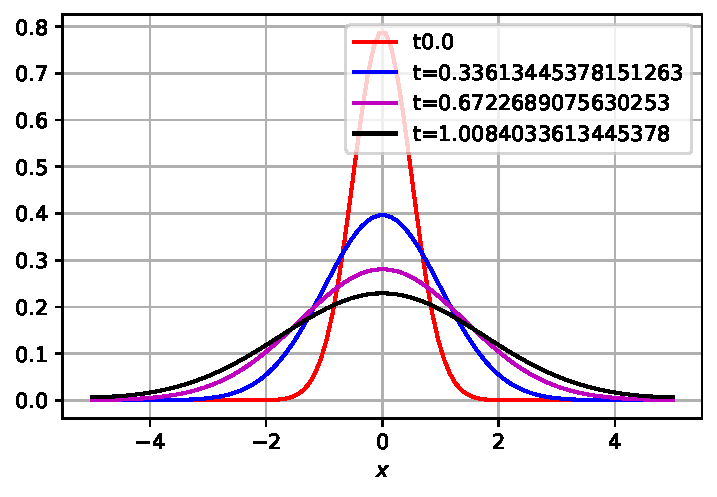
\includegraphics{linearreactiondiffusion_files/figure-pdf/fig-diffusionpde-output-2.pdf}

}

\caption{\label{fig-diffusionpde}Numerical solution of diffusion
equation.}

\end{figure}

\begin{figure}[H]

{\centering 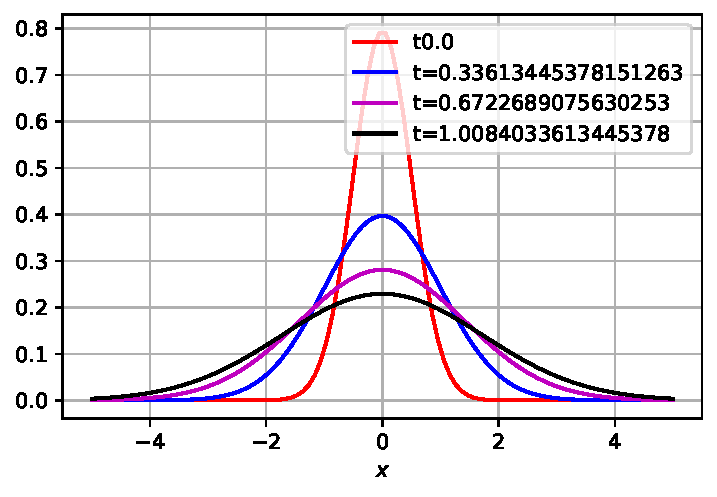
\includegraphics{linearreactiondiffusion_files/figure-pdf/fig-diffusionpde-output-3.pdf}

}

\caption{\label{fig-diffusionpde}Exact solution of diffusion equation.}

\end{figure}

\hypertarget{key-properties-of-the-linear-diffusion-equation-heat-equation}{%
\subsection{Key properties of the (linear) diffusion equation (heat
equation)}\label{key-properties-of-the-linear-diffusion-equation-heat-equation}}

\begin{itemize}
\tightlist
\item
  The solution is infinitely smooth.
\item
  The solution \(c(x,t)\) stays positive for all \(t >0\) and
  \(x \in \mathbb R\) if \(c(x,0) >0\) for \(x \in \mathbb R\).
\item
  The solution ``propagates'\,' with infinite speed i.e.~for any
  \(t > 0\), the solution is everywhere in \(\mathbb R\).
\item
  If we change the initial data \(c(x,0)\) (continuously) then the
  solution also changes (continuously).
\end{itemize}

\hypertarget{diffusive-transit-time}{%
\subsection{Diffusive transit time}\label{diffusive-transit-time}}

We now demonstrate the connection between time and space in diffusion
equations. Consider a domain \(V \subset \mathbb R^n \;, n = 1,2,3.\),
and particles that are entering \(V\) and are being removed from \(V\).
Define

\(N\) - total number of particles in \(V\)

\(F\) - total number of particles entering \(V\) per unit time

\(\lambda\) - average removal rate of particles from \(V\)

\(\tau = \frac 1\lambda\) - transit time or average time of residency in
\(V\)

Regardless of spatial variations, we can make the following general
statement regarding the total number of particles in \(V\), where we
assume a constant entry rate \(F\) and a constant removal rate
\(\lambda\) at some sink in \(V\):

\[
\frac{dN}{dt} = \text{entry rate} - \text{removal rate} = F - \lambda N.
\]

At steady state (\(dN/dt = 0\)) we obtain \[
Missing content here. Check notes!
\]

Consider particles of concentration \(c(x,t)\) diffusing with constant
diffusion \(D\) in a one-dimensional domain \((0,L)\), with a constant
concentration at one boundary and removed by a sink at the other
boundary. At steady-state, the equation governing the concentration is
given by:

\[
D \frac{ d^2 c}{dx^2} = 0  \quad \text{ in } (0,L), \quad c(0) = C_0, \, c(L) = 0 .
\]

The solution (\textbf{Exercise}) is: \[
c(x) = C_0 \left( 1- \frac x L\right).
\] Then the number of particles entering at \(x=0\) due to diffusive
flux (Fickian diffusion) is: \[
J = - D \frac{ dc}{ dx} = D \frac{ C_0} L,  
\]

and the total number of particles is given by: \[
N = \int_0^L c(x) \, dx = \frac 12 L C_0 .
\] If we assume a cross-section of unit area at \(x=0\), then \[
F = \text{flux}\times\text{area} = J\times 1 = D \frac{ C_0} L
\] and \[
\tau =  \frac N F = \frac { C_0 L}{2} \frac L{ DC_0} = \frac 12 \frac{L^2}{D}.
\] Thus the average time it takes a particle to diffuse a distance,
\(L\), is \[
\tau = \dfrac{L^2}{2D}
\] or viewed another way, the average distance through which diffusion
transports a particle in a time \(\tau\) is \(L= \sqrt{ 2D\tau}\).

\hypertarget{diffusion-as-the-limit-of-a-random-walk}{%
\subsection{Diffusion as the limit of a random
walk}\label{diffusion-as-the-limit-of-a-random-walk}}

Consider the \textbf{random walk} of particles in a one-dimensional
domain. Suppose that the particles move randomly a distance,
\(\Delta x\), every time step, \(\Delta t\). Assume that the particles
move left with probability \(\lambda_L\) and right with probability
\(\lambda_R\).

In Figure Figure~\ref{fig-randomwalksim} a simulation of 400 random
walking particles is presented. Each particle is initialised at the
origin and can move one step left or right with equal probability at
every time step of the simulation. As time evolves the particle density
(histogram) disperses. The normalised particle density appears to be
well described by the solution of the diffusion equation (solid lines,
Equation~\ref{eq-fund_sol}).

\begin{Shaded}
\begin{Highlighting}[]
\ImportTok{import}\NormalTok{ numpy }\ImportTok{as}\NormalTok{ np}
\ImportTok{from}\NormalTok{ scipy.integrate }\ImportTok{import}\NormalTok{ odeint}
\ImportTok{import}\NormalTok{ matplotlib.pyplot }\ImportTok{as}\NormalTok{ plt}
\ImportTok{import}\NormalTok{ random}

\NormalTok{N\_particles}\OperatorTok{=}\DecValTok{400}

\NormalTok{L}\OperatorTok{=}\DecValTok{50}
\NormalTok{N\_x}\OperatorTok{=}\DecValTok{200}

\NormalTok{T}\OperatorTok{=}\DecValTok{500}
\NormalTok{N\_t}\OperatorTok{=}\DecValTok{25000}
\NormalTok{D}\OperatorTok{=}\FloatTok{0.1}

\NormalTok{dt}\OperatorTok{=}\NormalTok{T}\OperatorTok{/}\NormalTok{N\_t}

\NormalTok{move\_probability}\OperatorTok{=}\NormalTok{D}\OperatorTok{*}\NormalTok{dt}\OperatorTok{/}\NormalTok{dx}\OperatorTok{**}\DecValTok{2}

\NormalTok{x}\OperatorTok{=}\NormalTok{np.linspace(}\DecValTok{0}\NormalTok{,L,N\_x)}\OperatorTok{{-}}\NormalTok{L}\OperatorTok{/}\DecValTok{2}
\NormalTok{t}\OperatorTok{=}\NormalTok{np.linspace(dt,T,N\_t)}

\NormalTok{particle\_positions}\OperatorTok{=}\NormalTok{np.zeros((N\_t,N\_particles),dtype}\OperatorTok{=}\BuiltInTok{float}\NormalTok{)}

\CommentTok{\# loop over time}
\ControlFlowTok{for}\NormalTok{ i }\KeywordTok{in} \BuiltInTok{range}\NormalTok{(}\DecValTok{1}\NormalTok{,N\_t):}
  \CommentTok{\# loop over particles}
  \ControlFlowTok{for}\NormalTok{ j }\KeywordTok{in} \BuiltInTok{range}\NormalTok{(N\_particles):}

\NormalTok{    r}\OperatorTok{=}\NormalTok{random.random()}
    \CommentTok{\# move particle j right}
\NormalTok{    new\_particle\_position}\OperatorTok{=}\NormalTok{particle\_positions[i}\OperatorTok{{-}}\DecValTok{1}\NormalTok{,j]}
    \ControlFlowTok{if}\NormalTok{ r}\OperatorTok{\textless{}}\NormalTok{move\_probability:}
\NormalTok{      new\_particle\_position}\OperatorTok{+=}\NormalTok{dx}
    \CommentTok{\# move particle j left  }
    \ControlFlowTok{elif}\NormalTok{ r}\OperatorTok{\textless{}}\DecValTok{2}\OperatorTok{*}\NormalTok{move\_probability:}
\NormalTok{      new\_particle\_position}\OperatorTok{{-}=}\NormalTok{dx}
\NormalTok{    particle\_positions[i,j]}\OperatorTok{=}\NormalTok{new\_particle\_position}


\NormalTok{[x\_mesh,t\_mesh]}\OperatorTok{=}\NormalTok{np.meshgrid(x,t)}
\NormalTok{c\_exact}\OperatorTok{=}\DecValTok{1}\OperatorTok{/}\NormalTok{np.sqrt(}\DecValTok{4}\OperatorTok{*}\NormalTok{np.pi}\OperatorTok{*}\NormalTok{D}\OperatorTok{*}\NormalTok{t\_mesh)}\OperatorTok{*}\NormalTok{np.exp(}\OperatorTok{{-}}\NormalTok{x\_mesh}\OperatorTok{**}\DecValTok{2}\OperatorTok{/}\NormalTok{(}\DecValTok{4}\OperatorTok{*}\NormalTok{D}\OperatorTok{*}\NormalTok{t\_mesh))}


\NormalTok{fig,ax}\OperatorTok{=}\NormalTok{plt.subplots(}\DecValTok{2}\NormalTok{,}\DecValTok{2}\NormalTok{)}
\NormalTok{ax[}\DecValTok{0}\NormalTok{,}\DecValTok{0}\NormalTok{].hist(particle\_positions[}\DecValTok{5}\NormalTok{,:],density}\OperatorTok{=}\VariableTok{True}\NormalTok{)}
\NormalTok{ax[}\DecValTok{0}\NormalTok{,}\DecValTok{0}\NormalTok{].plot(x, c\_exact[}\DecValTok{5}\NormalTok{,:], }\StringTok{\textquotesingle{}r\textquotesingle{}}\NormalTok{)}
\NormalTok{ax[}\DecValTok{0}\NormalTok{,}\DecValTok{0}\NormalTok{].set\_title(}\StringTok{\textquotesingle{}$t=$\textquotesingle{}}\OperatorTok{+}\BuiltInTok{str}\NormalTok{(t[}\DecValTok{5}\NormalTok{]))}

\NormalTok{ax[}\DecValTok{0}\NormalTok{,}\DecValTok{1}\NormalTok{].hist(particle\_positions[}\DecValTok{500}\NormalTok{,:],density}\OperatorTok{=}\VariableTok{True}\NormalTok{)}
\NormalTok{ax[}\DecValTok{0}\NormalTok{,}\DecValTok{1}\NormalTok{].plot(x, c\_exact[}\DecValTok{500}\NormalTok{,:], }\StringTok{\textquotesingle{}m\textquotesingle{}}\NormalTok{)}
\NormalTok{ax[}\DecValTok{0}\NormalTok{,}\DecValTok{1}\NormalTok{].set\_title(}\StringTok{\textquotesingle{}$t=$\textquotesingle{}}\OperatorTok{+}\BuiltInTok{str}\NormalTok{(t[}\DecValTok{500}\NormalTok{]))}

\NormalTok{ax[}\DecValTok{1}\NormalTok{,}\DecValTok{0}\NormalTok{].hist(particle\_positions[}\DecValTok{1000}\NormalTok{,:],density}\OperatorTok{=}\VariableTok{True}\NormalTok{)}
\NormalTok{ax[}\DecValTok{1}\NormalTok{,}\DecValTok{0}\NormalTok{].plot(x, c\_exact[}\DecValTok{1000}\NormalTok{,:], }\StringTok{\textquotesingle{}b\textquotesingle{}}\NormalTok{)}
\NormalTok{ax[}\DecValTok{1}\NormalTok{,}\DecValTok{0}\NormalTok{].set\_title(}\StringTok{\textquotesingle{}$t=$\textquotesingle{}}\OperatorTok{+}\BuiltInTok{str}\NormalTok{(t[}\DecValTok{1000}\NormalTok{]))}

\NormalTok{ax[}\DecValTok{1}\NormalTok{,}\DecValTok{1}\NormalTok{].hist(particle\_positions[}\DecValTok{1500}\NormalTok{,:],density}\OperatorTok{=}\VariableTok{True}\NormalTok{)}
\NormalTok{ax[}\DecValTok{1}\NormalTok{,}\DecValTok{1}\NormalTok{].plot(x, c\_exact[}\DecValTok{1500}\NormalTok{,:], }\StringTok{\textquotesingle{}k\textquotesingle{}}\NormalTok{)}
\NormalTok{ax[}\DecValTok{1}\NormalTok{,}\DecValTok{1}\NormalTok{].set\_title(}\StringTok{\textquotesingle{}$t=$\textquotesingle{}}\OperatorTok{+}\BuiltInTok{str}\NormalTok{(t[}\DecValTok{1500}\NormalTok{]))}

\NormalTok{ax[}\DecValTok{0}\NormalTok{,}\DecValTok{0}\NormalTok{].set\_xlim([}\OperatorTok{{-}}\NormalTok{L}\OperatorTok{/}\DecValTok{2}\NormalTok{,L}\OperatorTok{/}\DecValTok{2}\NormalTok{])}
\NormalTok{ax[}\DecValTok{0}\NormalTok{,}\DecValTok{1}\NormalTok{].set\_xlim([}\OperatorTok{{-}}\NormalTok{L}\OperatorTok{/}\DecValTok{2}\NormalTok{,L}\OperatorTok{/}\DecValTok{2}\NormalTok{])}
\NormalTok{ax[}\DecValTok{1}\NormalTok{,}\DecValTok{0}\NormalTok{].set\_xlim([}\OperatorTok{{-}}\NormalTok{L}\OperatorTok{/}\DecValTok{2}\NormalTok{,L}\OperatorTok{/}\DecValTok{2}\NormalTok{])}
\NormalTok{ax[}\DecValTok{1}\NormalTok{,}\DecValTok{1}\NormalTok{].set\_xlim([}\OperatorTok{{-}}\NormalTok{L}\OperatorTok{/}\DecValTok{2}\NormalTok{,L}\OperatorTok{/}\DecValTok{2}\NormalTok{])}
\NormalTok{plt.xlabel(}\StringTok{\textquotesingle{}$x$\textquotesingle{}}\NormalTok{)}
\NormalTok{plt.grid()}
\NormalTok{plt.show()}
\end{Highlighting}
\end{Shaded}

\begin{figure}[H]

{\centering 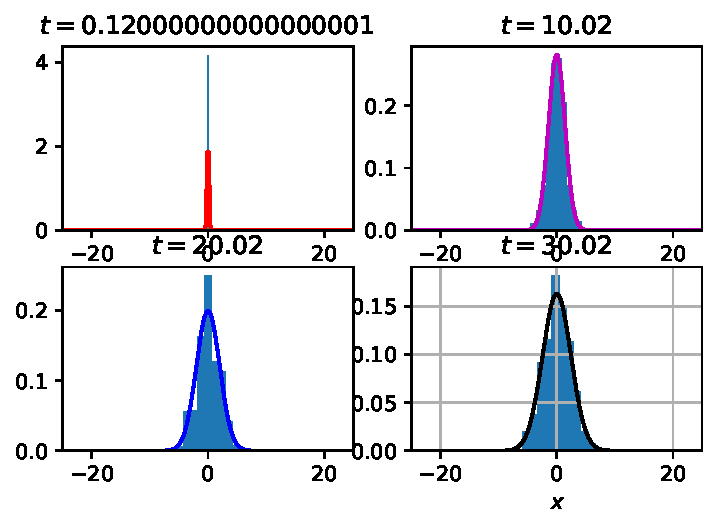
\includegraphics{linearreactiondiffusion_files/figure-pdf/fig-randomwalksim-output-1.pdf}

}

\caption{\label{fig-randomwalksim}Numerical implementation of random
walk}

\end{figure}

Concider the concentration of particles \(c(x,t)\) at spatial location
\(x\) and time \(t\), (or more precisely, the probability density
function of the position of a particle performing a random walk) we
have: \[
c(x, t+ \Delta t) = c(x, t)  + \lambda_R c(x- \Delta x, t) - \lambda_R c(x, t) + \lambda_L c(x+ \Delta x, t) - \lambda_L c (x,t).
\] If we assume that \(\lambda_R+ \lambda_L =1\) then \[
c(x, t+ \Delta t) =  \lambda_R c(x- \Delta x, t) + \lambda_L c(x+ \Delta x, t).
\] Applying a Taylor series expansion about \((x,t)\) implies

\[
c(t,x) + \frac{ \partial c}{\partial t} \Delta t + \frac 12  \frac{ \partial^2 c}{\partial^2 t} (\Delta t )^2  + h.o.t. =
\lambda_R \Big( c(t,x) - \frac{ \partial c}{\partial x} \Delta x + \frac 12  \frac{ \partial^2 c}{\partial^2 x} (\Delta x )^2  + h.o.t. \Big)\\ +
\lambda_L \Big( c(t,x) + \frac{ \partial c}{\partial x} \Delta x + \frac 12  \frac{ \partial^2 c}{\partial^2 x} (\Delta x )^2  + h.o.t. \Big).
\]

Using \(\lambda_R+ \lambda_L =1\) and assuming
\(\lambda_L = \lambda_R = \frac 12\) we obtain

\[
 \frac{ \partial c}{\partial t} \Delta t + \frac 12  \frac{ \partial^2 c}{\partial^2 t} (\Delta t )^2  + h.o.t. =
 \frac 12  \frac{ \partial^2 c}{\partial^2 x} (\Delta x )^2  + h.o.t. 
\] Dividing by \(\Delta t\) gives

\[
 \frac{ \partial c}{\partial t}  + \frac 12  \frac{ \partial^2 c}{\partial^2 t} \Delta t   + h.o.t. =
   \frac{ \partial^2 c}{\partial^2 x} \frac{(\Delta x )^2 }{2\Delta t} + h.o.t. 
\]

Considering the limit \(\Delta t \to 0\) and \(\Delta x \to 0\) in such
way that

\[
 \frac{(\Delta x )^2 }{2\Delta t} \to D,
\]

yields the (one-dimensional) diffusion equation

\[
\frac{\partial c}{\partial t} = D \frac{\partial^2 c}{\partial x^2}.
\]

This approach can be extended to consider other types of movement
e.g.~convection. For example, if we assume that\\
\[
\lambda_R+ \lambda_L =1,
\] and \[
\lambda_L - \lambda_R = \varepsilon,
\] the motion of the particles is biased and we may derive an
appropriate \textbf{reaction-diffusion-convection} equation (see
tutorial).

Finally we note that there is a connection between diffusion and the
normal distribution function.

\textbf{Recall} The normal distribution function in one-dimension with
zero mean and variance \(\sigma^2\) is given by @\#eq-fund\_sol.

\[
N(0, \sigma^2) \sim \frac 1 { \sqrt{ 2 \pi \sigma^2}} \exp \left( - \frac{x^2}{ 2 \sigma^2}\right).
\] Examining the formula for the fundamental solution of the diffusion
Equation~\ref{eq-fund_sol} in one-dimension, we see by inspection that
the probability density function of the position of a particle
performing a random walk in one-dimension starting at the origin is
normally distributed with mean zero and variance \[
\sigma^2 = 2 D t.
\]

\hypertarget{linear-reaction-diffusion-equations-1}{%
\section{Linear reaction-diffusion
equations}\label{linear-reaction-diffusion-equations-1}}

Consider now the linear reaction term: \(f(c) = \rho c\), so that our
reaction-diffusion equation is:
\begin{equation}\protect\hypertarget{eq-lin_re_eq}{}{
\frac{\partial c}{\partial t} = D \frac{\partial^2 c}{\partial x^2}   + \rho \, c, \quad x\in \mathbb R, \, \, t >0, 
}\label{eq-lin_re_eq}\end{equation} where \(\rho \in \mathbb R\) is a
constant.

Once again we consider the initial condition to be concentrated at the
origin: \begin{equation}\protect\hypertarget{eq-lin_re_eq_ic}{}{
c(0,x) = \delta_0(x).
}\label{eq-lin_re_eq_ic}\end{equation}

\hypertarget{exact-solution}{%
\subsection{Exact solution}\label{exact-solution}}

By considering a \emph{separation of variables} approach, i.e.~making
the \textbf{ansatz} \[
c(x,t) = w(t) \tilde c(t,x),
\] it can be shown (\textbf{Exercise}) that the explicit solution for
the linear reaction-diffusion Equation~\ref{eq-lin_re_eq} with initial
condition Equation~\ref{eq-lin_re_eq_ic} is given by

\[
c(t,x) = \frac1{\sqrt{4 \pi D t}} \exp \left(\rho t - \frac{x^2}{ 4Dt} \right).
\]

\begin{Shaded}
\begin{Highlighting}[]
\ImportTok{import}\NormalTok{ numpy }\ImportTok{as}\NormalTok{ np}
\ImportTok{from}\NormalTok{ scipy.integrate }\ImportTok{import}\NormalTok{ odeint}
\ImportTok{import}\NormalTok{ matplotlib.pyplot }\ImportTok{as}\NormalTok{ plt}

\NormalTok{T}\OperatorTok{=}\DecValTok{10}
\NormalTok{L}\OperatorTok{=}\DecValTok{10}

\NormalTok{N\_x}\OperatorTok{=}\DecValTok{100}
\NormalTok{N\_t}\OperatorTok{=}\DecValTok{120}

\NormalTok{t}\OperatorTok{=}\NormalTok{np.linspace(}\DecValTok{0}\NormalTok{,T,N\_t)}
\NormalTok{x}\OperatorTok{=}\NormalTok{np.linspace(}\DecValTok{0}\NormalTok{,L,N\_x)}\OperatorTok{{-}}\NormalTok{L}\OperatorTok{/}\DecValTok{2}

\NormalTok{D}\OperatorTok{=}\FloatTok{0.5}
\NormalTok{rho}\OperatorTok{=}\FloatTok{1.0}
\NormalTok{epsilon}\OperatorTok{=}\FloatTok{0.1}

\NormalTok{u\_0}\OperatorTok{=}\DecValTok{1}\OperatorTok{/}\NormalTok{(epsilon}\OperatorTok{*}\NormalTok{np.sqrt(np.pi))}\OperatorTok{*}\NormalTok{np.exp(}\OperatorTok{{-}}\NormalTok{x}\OperatorTok{**}\DecValTok{2}\OperatorTok{/}\NormalTok{epsilon}\OperatorTok{**}\DecValTok{2}\NormalTok{)}

\NormalTok{dx}\OperatorTok{=}\NormalTok{L}\OperatorTok{/}\NormalTok{(N\_x}\OperatorTok{{-}}\DecValTok{1}\NormalTok{)}
\NormalTok{dt}\OperatorTok{=}\NormalTok{T}\OperatorTok{/}\NormalTok{(N\_t}\OperatorTok{{-}}\DecValTok{1}\NormalTok{)}


\KeywordTok{def}\NormalTok{ logisticPDErhs(u,t):}
\NormalTok{    N\_x}\OperatorTok{=}\BuiltInTok{len}\NormalTok{(u)}
\NormalTok{    f}\OperatorTok{=}\NormalTok{np.zeros\_like(u)}
    \ControlFlowTok{for}\NormalTok{ i }\KeywordTok{in} \BuiltInTok{range}\NormalTok{(}\DecValTok{1}\NormalTok{,N\_x}\OperatorTok{{-}}\DecValTok{1}\NormalTok{):}
\NormalTok{      f[i]}\OperatorTok{=}\NormalTok{D}\OperatorTok{/}\NormalTok{dx}\OperatorTok{**}\DecValTok{2}\OperatorTok{*}\NormalTok{(u[i}\OperatorTok{{-}}\DecValTok{1}\NormalTok{]}\OperatorTok{{-}}\DecValTok{2}\OperatorTok{*}\NormalTok{u[i]}\OperatorTok{+}\NormalTok{u[i}\OperatorTok{+}\DecValTok{1}\NormalTok{])  }


\NormalTok{    i}\OperatorTok{=}\DecValTok{0}
\NormalTok{    f[i]}\OperatorTok{=}\NormalTok{D}\OperatorTok{/}\NormalTok{dx}\OperatorTok{**}\DecValTok{2}\OperatorTok{*}\NormalTok{(}\OperatorTok{{-}}\NormalTok{u[i]}\OperatorTok{+}\NormalTok{u[i}\OperatorTok{+}\DecValTok{1}\NormalTok{])}
\NormalTok{    i}\OperatorTok{=}\NormalTok{N\_x}\OperatorTok{{-}}\DecValTok{1}

\NormalTok{    f[i]}\OperatorTok{=}\NormalTok{D}\OperatorTok{/}\NormalTok{dx}\OperatorTok{**}\DecValTok{2}\OperatorTok{*}\NormalTok{(u[i}\OperatorTok{{-}}\DecValTok{1}\NormalTok{]}\OperatorTok{{-}}\NormalTok{u[i])}

\NormalTok{    reac}\OperatorTok{=}\NormalTok{rho}\OperatorTok{*}\NormalTok{u}
\NormalTok{    f}\OperatorTok{=}\NormalTok{f}\OperatorTok{+}\NormalTok{reac}
    \ControlFlowTok{return}\NormalTok{ f  }

\NormalTok{sol}\OperatorTok{=}\NormalTok{odeint(logisticPDErhs,u\_0,t)}


\NormalTok{[x\_mesh,t\_mesh]}\OperatorTok{=}\NormalTok{np.meshgrid(x,t)}

\NormalTok{c\_exact}\OperatorTok{=}\DecValTok{1}\OperatorTok{/}\NormalTok{np.sqrt(}\DecValTok{4}\OperatorTok{*}\NormalTok{np.pi}\OperatorTok{*}\NormalTok{D}\OperatorTok{*}\NormalTok{t\_mesh)}\OperatorTok{*}\NormalTok{np.exp(rho}\OperatorTok{*}\NormalTok{t\_mesh}\OperatorTok{{-}}\NormalTok{x\_mesh}\OperatorTok{**}\DecValTok{2}\OperatorTok{/}\NormalTok{(}\DecValTok{4}\OperatorTok{*}\NormalTok{D}\OperatorTok{*}\NormalTok{t\_mesh))}

\NormalTok{fig,ax}\OperatorTok{=}\NormalTok{plt.subplots()}
\NormalTok{ax.plot(x, sol[}\DecValTok{1}\NormalTok{,:], }\StringTok{\textquotesingle{}r\textquotesingle{}}\NormalTok{)}
\NormalTok{ax.plot(x, sol[}\DecValTok{4}\NormalTok{,:], }\StringTok{\textquotesingle{}b\textquotesingle{}}\NormalTok{)}
\NormalTok{ax.plot(x, sol[}\DecValTok{8}\NormalTok{,:], }\StringTok{\textquotesingle{}m\textquotesingle{}}\NormalTok{)}
\NormalTok{ax.plot(x, sol[}\DecValTok{12}\NormalTok{,:], }\StringTok{\textquotesingle{}k\textquotesingle{}}\NormalTok{)}
\NormalTok{plt.legend([}\StringTok{\textquotesingle{}t\textquotesingle{}}\OperatorTok{+} \BuiltInTok{str}\NormalTok{(t[}\DecValTok{0}\NormalTok{]),}\StringTok{\textquotesingle{}t=\textquotesingle{}}\OperatorTok{+} \BuiltInTok{str}\NormalTok{(t[}\DecValTok{4}\NormalTok{]),}\StringTok{\textquotesingle{}t=\textquotesingle{}}\OperatorTok{+} \BuiltInTok{str}\NormalTok{(t[}\DecValTok{8}\NormalTok{]),}\StringTok{\textquotesingle{}t=\textquotesingle{}}\OperatorTok{+} \BuiltInTok{str}\NormalTok{(t[}\DecValTok{12}\NormalTok{])])}
\NormalTok{plt.xlabel(}\StringTok{\textquotesingle{}$x$\textquotesingle{}}\NormalTok{)}
\NormalTok{plt.grid()}
\NormalTok{plt.show()}

\NormalTok{fig,ax}\OperatorTok{=}\NormalTok{plt.subplots()}
\NormalTok{ax.plot(x, c\_exact[}\DecValTok{1}\NormalTok{,:], }\StringTok{\textquotesingle{}r\textquotesingle{}}\NormalTok{)}
\NormalTok{ax.plot(x, c\_exact[}\DecValTok{4}\NormalTok{,:], }\StringTok{\textquotesingle{}b\textquotesingle{}}\NormalTok{)}
\NormalTok{ax.plot(x, c\_exact[}\DecValTok{8}\NormalTok{,:], }\StringTok{\textquotesingle{}m\textquotesingle{}}\NormalTok{)}
\NormalTok{ax.plot(x, c\_exact[}\DecValTok{12}\NormalTok{,:], }\StringTok{\textquotesingle{}k\textquotesingle{}}\NormalTok{)}
\NormalTok{plt.legend([}\StringTok{\textquotesingle{}t\textquotesingle{}}\OperatorTok{+} \BuiltInTok{str}\NormalTok{(t[}\DecValTok{0}\NormalTok{]),}\StringTok{\textquotesingle{}t=\textquotesingle{}}\OperatorTok{+} \BuiltInTok{str}\NormalTok{(t[}\DecValTok{4}\NormalTok{]),}\StringTok{\textquotesingle{}t=\textquotesingle{}}\OperatorTok{+} \BuiltInTok{str}\NormalTok{(t[}\DecValTok{8}\NormalTok{]),}\StringTok{\textquotesingle{}t=\textquotesingle{}}\OperatorTok{+} \BuiltInTok{str}\NormalTok{(t[}\DecValTok{12}\NormalTok{])])}
\NormalTok{plt.xlabel(}\StringTok{\textquotesingle{}$x$\textquotesingle{}}\NormalTok{)}
\NormalTok{plt.grid()}
\NormalTok{plt.show()}
\end{Highlighting}
\end{Shaded}

\begin{verbatim}
/var/folders/m_/vc0kz_0x6ls5n4qnksq052jw0000gp/T/ipykernel_21338/3455521560.py:46: RuntimeWarning:

divide by zero encountered in divide

/var/folders/m_/vc0kz_0x6ls5n4qnksq052jw0000gp/T/ipykernel_21338/3455521560.py:46: RuntimeWarning:

invalid value encountered in multiply
\end{verbatim}

\begin{figure}[H]

{\centering 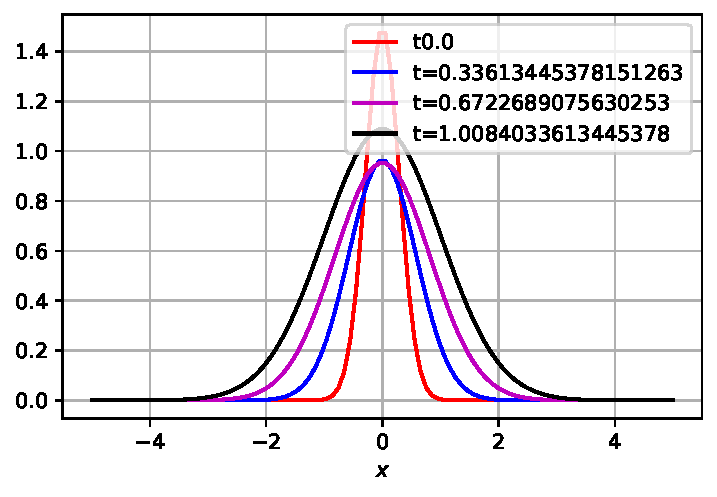
\includegraphics{linearreactiondiffusion_files/figure-pdf/fig-diffusionlinearsource-output-2.pdf}

}

\caption{\label{fig-diffusionlinearsource}Numerical solution of linear
reaction diffusion equation}

\end{figure}

\begin{figure}[H]

{\centering 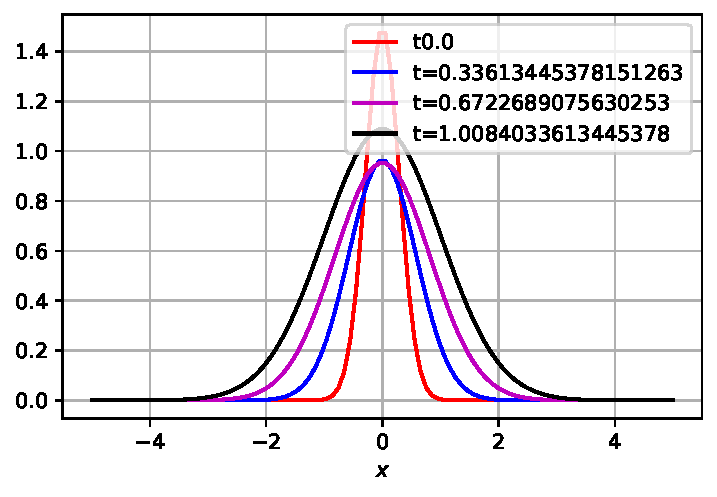
\includegraphics{linearreactiondiffusion_files/figure-pdf/fig-diffusionlinearsource-output-3.pdf}

}

\caption{\label{fig-diffusionlinearsource}Exact solution of linear
reaction diffusion equation}

\end{figure}

\hypertarget{speed-of-a-wave-of-invasion}{%
\subsection{Speed of a wave of
invasion}\label{speed-of-a-wave-of-invasion}}

Muskrats which were introduced in 1905 in Bohemia initially spread
rapidly throughout Europe through a combination of random movement and
proliferation (initially there were no predators and proliferation was
rapid). A model for the initial spread can therefore be given by a
two-dimensional diffusion equation combined with exponential growth and
assuming that \(M\) individuals were released at the origin (i.e.~in
Bohemia). Considering the density of muskrats \(u({\mathbf{x}} , t)\),
the equation is

\begin{equation}\protect\hypertarget{eq-muskrats_eq}{}{
\frac{\partial u}{\partial t} = D \left(\frac{\partial^2 u}{\partial x_1^2} +  \frac{\partial^2 u}{\partial x_2^2}\right)  + \rho \, u, \quad {\mathbf{x}} = (x_1 , x_2) \in \mathbb R^2, \, \, t >0, 
}\label{eq-muskrats_eq}\end{equation}
\begin{equation}\protect\hypertarget{eq-muskrats_eq_in}{}{
u({\mathbf{x}}, 0) = M \delta_0({\mathbf{x}}), \quad {\mathbf{x}} \in \mathbb R^2.
}\label{eq-muskrats_eq_in}\end{equation}

The solution of Equation~\ref{eq-muskrats_eq} with initial conditions
Equation~\ref{eq-muskrats_eq_in} is equal to:

\[
u({\mathbf{x}}, t) = \frac M{4 \pi D t} \exp \left(\rho t - \frac{ |{\mathbf{x}} |^2}{ 4Dt} \right)\; = \frac M{4 \pi D t} \exp \left(\rho t - \frac{ (x_{1}^{2} + x_{2}^{2})}{4Dt} \right).
\]

Transforming to polar coordinates \(x_1 = r \cos\varphi\),
\(x_2 = r \sin \varphi\) we obtain

\[
u({\mathbf{x}}, t) = \frac M{4 \pi D t} \exp \left(\rho t - \frac{ r^2}{ 4Dt} \right).
\]

From the properties of the fundamental solution, the wave of invasion
extends all the way to infinity if \(t>0\). Thus, for practical
purposes, somehow we have to define the front of the wave.

Consider that there is some detection threshold for the muskrats
i.e.~some predetermined small value of the density \(u_1\), say, such
that any changes in density for \(u <u_1\) cannot be detected.

Because of the symmetry of the problem, then the leading edge of the
invading wave front of muskrats is the circle of radius \(r=r_1(t)\)
where \(u=u_1\), i.e.~from the explicit solution of
Equation~\ref{eq-muskrats_eq},

\[
u_1({\mathbf{x}}, t) = \frac M{4 \pi D t} \exp \left(\rho t - \frac{ r_1^2}{ 4Dt} \right).
\]

Rearranging and solving for \(r_1\), using the fact that \[
\lim\limits_{t\to \infty} \dfrac {\ln t} t =0, 
\] we obtain for large \(t\) that \[
r_1(t) \approx 2 \sqrt{ \rho D} t.
\]

Hence, the speed of invasion of the leading edge of the muskrats is
given by: \[
v = \frac{r_1(t)}{t} =  2 \sqrt{ \rho D}. 
\]

\hypertarget{non-linear-reaction-diffusion-equations}{%
\chapter{Non linear reaction diffusion
equations}\label{non-linear-reaction-diffusion-equations}}

We now consider the one-dimensional diffusion equation with a non-linear
reaction term of ``logistic growth'', to give the nonlinear
reaction-diffusion equation:

\begin{equation}\protect\hypertarget{eq-fisher}{}{
\frac{\partial u}{\partial t} = D\frac{\partial^2 u}{\partial x^2} +   \rho u\left(1-\frac u K\right), \qquad x\in \mathbb R, \, \, t >0,  
}\label{eq-fisher}\end{equation}

with initial Condition \[
u(x,0) =u_0(x). 
\]

This is known as \textbf{the Fisher equation}, and was introduced by
Fisher in \(1937\) ({``The Wave of Advance of Advantageous Genes''}
(1937)).

We can non-dimensionalize Equation~\ref{eq-fisher} by considering the
scaling
\[t^\ast = \rho t, \quad  x^\ast = \sqrt{\dfrac \rho D} x, \quad  u^\ast = \displaystyle{\frac u K}.
\] Dropping the asteriks we obtain the non-dimensionalized Fisher
equation (\textbf{Exercise}):

\[
\frac{\partial u}{\partial t} = \frac{\partial^2 u}{\partial x^2} +   u(1-u), \qquad x\in \mathbb R, \, \, t >0 
\] with initial condition
\begin{equation}\protect\hypertarget{eq-fisher_1}{}{
u(x,0) = u_0(x).
}\label{eq-fisher_1}\end{equation}

\hypertarget{numerical-solutions}{%
\section{Numerical solutions}\label{numerical-solutions}}

In Figure~\ref{fig-logisticpde} we have computed a numerical solution to
Equation~\ref{eq-fisher_1} together with no-flux boundary conditions.
See Python code for further details. The key point to note is that the
numerical solutions appear to be a \emph{travelling wave}, at successive
times the solution is translated along the \(x\) axis. At long times the
solution tends to \(u\sim1\) (behind the wavefront). Ahead of the front,
the solution is \(u\sim0\).

\begin{itemize}
\tightlist
\item
  Can we prove this is a travelling wave (e.g.~the solution could be
  dynamic on a very slow time scale that is not captured by the
  numeircal solution)?
\item
  Can we derived a form for the travelling wave profile?
\item
  Will we see a travelling wave for any initial data?
\item
  How does the wave speed relate to model parameters?
\end{itemize}

\begin{Shaded}
\begin{Highlighting}[]
\ImportTok{import}\NormalTok{ numpy }\ImportTok{as}\NormalTok{ np}
\ImportTok{from}\NormalTok{ scipy.integrate }\ImportTok{import}\NormalTok{ odeint}
\ImportTok{import}\NormalTok{ matplotlib.pyplot }\ImportTok{as}\NormalTok{ plt}

\NormalTok{T}\OperatorTok{=}\DecValTok{100}
\NormalTok{L}\OperatorTok{=}\DecValTok{100}

\NormalTok{N\_x}\OperatorTok{=}\DecValTok{100}
\NormalTok{N\_t}\OperatorTok{=}\DecValTok{100}

\NormalTok{t}\OperatorTok{=}\NormalTok{np.linspace(}\DecValTok{1}\NormalTok{,T,N\_t)}
\NormalTok{x}\OperatorTok{=}\NormalTok{np.linspace(}\DecValTok{0}\NormalTok{,L,N\_x)}


\NormalTok{u\_0}\OperatorTok{=}\FloatTok{0.5}\OperatorTok{*}\NormalTok{(}\DecValTok{1}\OperatorTok{+}\NormalTok{np.tanh(}\OperatorTok{{-}}\FloatTok{0.1}\OperatorTok{*}\NormalTok{(x}\OperatorTok{{-}}\DecValTok{20}\NormalTok{)))}

\NormalTok{dx}\OperatorTok{=}\NormalTok{L}\OperatorTok{/}\NormalTok{(N\_x}\OperatorTok{{-}}\DecValTok{1}\NormalTok{)}
\NormalTok{dt}\OperatorTok{=}\NormalTok{T}\OperatorTok{/}\NormalTok{(N\_t}\OperatorTok{{-}}\DecValTok{1}\NormalTok{)}


\KeywordTok{def}\NormalTok{ logisticPDErhs(u,t):}
\NormalTok{    N\_x}\OperatorTok{=}\BuiltInTok{len}\NormalTok{(u)}
\NormalTok{    f}\OperatorTok{=}\NormalTok{np.zeros\_like(u)}
    \ControlFlowTok{for}\NormalTok{ i }\KeywordTok{in} \BuiltInTok{range}\NormalTok{(}\DecValTok{1}\NormalTok{,N\_x}\OperatorTok{{-}}\DecValTok{1}\NormalTok{):}
\NormalTok{      f[i]}\OperatorTok{=}\DecValTok{1}\OperatorTok{/}\NormalTok{dx}\OperatorTok{**}\DecValTok{2}\OperatorTok{*}\NormalTok{(u[i}\OperatorTok{{-}}\DecValTok{1}\NormalTok{]}\OperatorTok{{-}}\DecValTok{2}\OperatorTok{*}\NormalTok{u[i]}\OperatorTok{+}\NormalTok{u[i}\OperatorTok{+}\DecValTok{1}\NormalTok{])}\OperatorTok{+}\NormalTok{u[i]}\OperatorTok{*}\NormalTok{(}\DecValTok{1}\OperatorTok{{-}}\NormalTok{u[i])  }


\NormalTok{    i}\OperatorTok{=}\DecValTok{0}
\NormalTok{    f[i]}\OperatorTok{=}\DecValTok{1}\OperatorTok{/}\NormalTok{dx}\OperatorTok{**}\DecValTok{2}\OperatorTok{*}\NormalTok{(}\OperatorTok{{-}}\NormalTok{u[i]}\OperatorTok{+}\NormalTok{u[i}\OperatorTok{+}\DecValTok{1}\NormalTok{])}\OperatorTok{+}\NormalTok{u[i]}\OperatorTok{*}\NormalTok{(}\DecValTok{1}\OperatorTok{{-}}\NormalTok{u[i]) }
\NormalTok{    i}\OperatorTok{=}\NormalTok{N\_x}\OperatorTok{{-}}\DecValTok{1}

\NormalTok{    f[i]}\OperatorTok{=}\DecValTok{1}\OperatorTok{/}\NormalTok{dx}\OperatorTok{**}\DecValTok{2}\OperatorTok{*}\NormalTok{(u[i}\OperatorTok{{-}}\DecValTok{1}\NormalTok{]}\OperatorTok{{-}}\NormalTok{u[i])}\OperatorTok{+}\NormalTok{u[i]}\OperatorTok{*}\NormalTok{(}\DecValTok{1}\OperatorTok{{-}}\NormalTok{u[i]) }
    \ControlFlowTok{return}\NormalTok{ f  }

\NormalTok{sol}\OperatorTok{=}\NormalTok{odeint(logisticPDErhs,u\_0,t)}

\NormalTok{plt.plot(x, sol[}\DecValTok{0}\NormalTok{,:], }\StringTok{\textquotesingle{}r\textquotesingle{}}\NormalTok{)}
\NormalTok{plt.plot(x, sol[}\DecValTok{4}\NormalTok{,:], }\StringTok{\textquotesingle{}b\textquotesingle{}}\NormalTok{)}
\NormalTok{plt.plot(x, sol[}\DecValTok{8}\NormalTok{,:], }\StringTok{\textquotesingle{}m\textquotesingle{}}\NormalTok{)}
\NormalTok{plt.plot(x, sol[}\DecValTok{12}\NormalTok{,:], }\StringTok{\textquotesingle{}k\textquotesingle{}}\NormalTok{)}
\NormalTok{plt.legend([}\StringTok{\textquotesingle{}t\textquotesingle{}}\OperatorTok{+} \BuiltInTok{str}\NormalTok{(t[}\DecValTok{0}\NormalTok{]),}\StringTok{\textquotesingle{}t=\textquotesingle{}}\OperatorTok{+} \BuiltInTok{str}\NormalTok{(t[}\DecValTok{4}\NormalTok{]),}\StringTok{\textquotesingle{}t=\textquotesingle{}}\OperatorTok{+} \BuiltInTok{str}\NormalTok{(t[}\DecValTok{8}\NormalTok{]),}\StringTok{\textquotesingle{}t=\textquotesingle{}}\OperatorTok{+} \BuiltInTok{str}\NormalTok{(t[}\DecValTok{12}\NormalTok{])])}
\NormalTok{plt.xlabel(}\StringTok{\textquotesingle{}$x$\textquotesingle{}}\NormalTok{)}
\NormalTok{plt.grid()}
\NormalTok{plt.show()}
\end{Highlighting}
\end{Shaded}

\begin{figure}[H]

{\centering 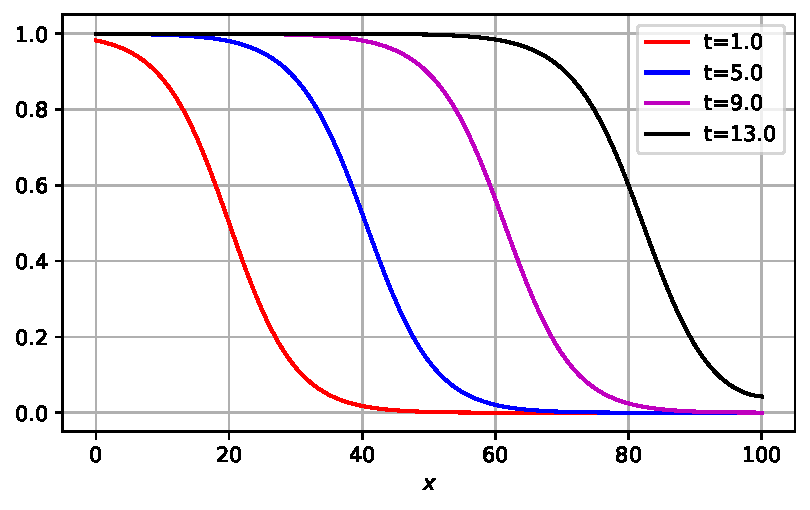
\includegraphics{nonlinearreactiondiffusion_files/figure-pdf/fig-logisticpde-output-1.pdf}

}

\caption{\label{fig-logisticpde}Numerical solution of Fisher's
equation.}

\end{figure}

\hypertarget{travelling-waves}{%
\section{Travelling waves}\label{travelling-waves}}

It is known that the Fisher Equation~\ref{eq-fisher_1} exhibits what are
known as \emph{travelling wave} solutions.

\begin{definition}[]\protect\hypertarget{def-trwave}{}\label{def-trwave}

A travelling wave is a solution of a partial differential equation with
a constant profile (shape) and a constant propagation speed.

\end{definition}

\hypertarget{types-of-travelling-waves}{%
\subsection{Types of travelling waves}\label{types-of-travelling-waves}}

\begin{itemize}
\tightlist
\item
  Travelling pulse: \(u(x,t) \to a\), as \(x \to \pm \infty\).
\item
  Travelling front : \(u(x,t) \to a\), as \(x \to - \infty\),
  \(u(x,t) \to b\), as \(x \to + \infty\) and \(a\neq b\) (this is what
  we see in Figure~\ref{fig-logisticpde})
\item
  Travelling train: \(u(x,t)\) is a periodic function in \(x\).
\end{itemize}

A travelling wave solution of a PDE can be written in the form
\(u(x,t) = W(z)\), where \(z = x - vt\). We shall consider \(v>0\),
which describes a wave moving from left to right.

Consider first the \emph{spatially uniform (homogeneous)} solution of
Equation~\ref{eq-fisher_1}

\begin{equation}\protect\hypertarget{eq-fisher_unif}{}{ 
\frac{\partial u}{\partial t} =    u(1-u), \qquad   \, \, t >0.
}\label{eq-fisher_unif}\end{equation}

Steady states of Equation~\ref{eq-fisher_unif} are \[
u=u_1 =1
\] and \[
u=u_2 =0.
\] To analyse the stability we consider \[
f(u)=u(1-u) \quad \textrm{and} \quad \frac{ df}{du}(u)= 1 - 2u.
\] Then \[
\frac{ df}{du}(u_1)= -1 \quad \textrm{and} \quad \frac{ df}{du}(u_2)= 1.
\] Thus \(u_1=1\) is \emph{stable} and \(u_2=0\) is \emph{unstable}.

This stability analysis suggests that for the spatially dependent
situation we can have a travelling wave solution that connects the two
steady states \(u_1\) and \(u_2\) i.e.~a travelling front.

Consider the travelling wave \emph{ansatz}\\
\[
u(x,t)= W(z) = W(x-vt),
\] where \(v\) is a constant. Changing variables in
Equation~\ref{eq-fisher_1} and using \[
\begin{aligned}
\frac{ \partial u}{\partial t} &= \frac{ dW}{dz} \frac{\partial z}{\partial t} = - v   \frac{ dW}{dz}, \\
 \frac{ \partial u}{\partial x} &= \frac{ dW}{dz} \frac{\partial z}{\partial x} =\frac{ dW}{dz}, \\
 \frac{ \partial^2 u}{\partial x^2} &= \frac{ d^2W}{dz^2} \left(\frac{\partial z}{\partial x} \right)^2 +  \frac{ dW}{dz} \frac{\partial^2 z}{\partial x^2} =\frac{ d^2W}{dz^2},
\end{aligned}
\]

we obtain a second order ordinary differential equation for \(W\)

\begin{equation}\protect\hypertarget{eq-tw_eq}{}{
\frac{ d^2W}{dz^2}+  v \frac{ dW}{dz} + W(1-W)  = 0, 
}\label{eq-tw_eq}\end{equation} where
\begin{equation}\protect\hypertarget{eq-tw_bc}{}{
W(z) \to 1 \quad \text{ as } \quad z \to  - \infty, \quad 
W(z) \to 0 \quad \text{ as } \quad z \to  +\infty,
}\label{eq-tw_bc}\end{equation} and
\begin{equation}\protect\hypertarget{eq-tw_r}{}{
W(z) \in [0,1]. 
}\label{eq-tw_r}\end{equation}

We can rewrite Equation~\ref{eq-tw_eq} as a system of two first order
ODEs

\begin{equation}\protect\hypertarget{eq-tw_eq_2}{}{
\begin{aligned}
\frac{ dW}{dz}& = P  = F(W,P), \\
\frac{ d P}{dz}&= -  v P - W(1-W)  = G(W,P).  
\end{aligned}
}\label{eq-tw_eq_2}\end{equation}

\hypertarget{numerical-solutions-1}{%
\subsection{Numerical solutions}\label{numerical-solutions-1}}

In Figure~\ref{fig-fishernumtravwave} we plot the numerical solution to
equations Equation~\ref{eq-tw_eq_2} for different values of the
wavespeed, \(v\). Note that when the wavespeed is too small the solution
spirals in towards the origin. This solution cannot be valid as it
implies that \(u<0\) for some \(z\).

Note that some problem will not have a travelling wave solution. In this
situation we could still make the travelling wave ansatz but this would
usually result in a contradiction. In such a case this tells us that a
travelling wave solution is not possible.

\begin{Shaded}
\begin{Highlighting}[]
\ImportTok{import}\NormalTok{ numpy }\ImportTok{as}\NormalTok{ np}
\ImportTok{from}\NormalTok{ scipy.integrate }\ImportTok{import}\NormalTok{ odeint}
\ImportTok{import}\NormalTok{ matplotlib.pyplot }\ImportTok{as}\NormalTok{ plt}

\NormalTok{T}\OperatorTok{=}\DecValTok{300}

\NormalTok{a}\OperatorTok{=}\FloatTok{0.2}
\NormalTok{N\_z}\OperatorTok{=}\DecValTok{5000}

\NormalTok{z}\OperatorTok{=}\NormalTok{np.linspace(}\DecValTok{1}\NormalTok{,T,N\_z)}

\NormalTok{u\_0}\OperatorTok{=}\NormalTok{[}\FloatTok{0.99}\NormalTok{,}\OperatorTok{{-}}\FloatTok{0.0001}\NormalTok{]}

\NormalTok{c\_1}\OperatorTok{=}\FloatTok{2.0}
\NormalTok{c\_2}\OperatorTok{=}\FloatTok{8.6}
\NormalTok{c\_3}\OperatorTok{=}\FloatTok{0.5}

\KeywordTok{def}\NormalTok{ fisherTrWaveODErhs(u, t, c):}
\NormalTok{    f}\OperatorTok{=}\NormalTok{np.zeros\_like(u)}
\NormalTok{    reaction}\OperatorTok{=}\NormalTok{u[}\DecValTok{0}\NormalTok{]}\OperatorTok{*}\NormalTok{(}\DecValTok{1}\OperatorTok{{-}}\NormalTok{u[}\DecValTok{0}\NormalTok{]) }

\NormalTok{    f[}\DecValTok{0}\NormalTok{]}\OperatorTok{=}\NormalTok{u[}\DecValTok{1}\NormalTok{]}
\NormalTok{    f[}\DecValTok{1}\NormalTok{]}\OperatorTok{={-}}\NormalTok{c}\OperatorTok{*}\NormalTok{u[}\DecValTok{1}\NormalTok{]}\OperatorTok{{-}}\NormalTok{reaction}
    \ControlFlowTok{return}\NormalTok{ f  }

\NormalTok{sol}\OperatorTok{=}\NormalTok{odeint(fisherTrWaveODErhs,u\_0,z, args}\OperatorTok{=}\NormalTok{(c\_1,))}
\NormalTok{sol2}\OperatorTok{=}\NormalTok{odeint(fisherTrWaveODErhs,u\_0,z, args}\OperatorTok{=}\NormalTok{(c\_2,))}
\NormalTok{sol3}\OperatorTok{=}\NormalTok{odeint(fisherTrWaveODErhs,u\_0,z, args}\OperatorTok{=}\NormalTok{(c\_3,))}

\NormalTok{fig, ax }\OperatorTok{=}\NormalTok{ plt.subplots(}\DecValTok{1}\NormalTok{,}\DecValTok{2}\NormalTok{)}
\NormalTok{ax[}\DecValTok{0}\NormalTok{].plot(sol[:,}\DecValTok{0}\NormalTok{],sol[:,}\DecValTok{1}\NormalTok{], }\StringTok{\textquotesingle{}r\textquotesingle{}}\NormalTok{)}
\NormalTok{ax[}\DecValTok{0}\NormalTok{].plot(sol2[:,}\DecValTok{0}\NormalTok{],sol2[:,}\DecValTok{1}\NormalTok{], }\StringTok{\textquotesingle{}b\textquotesingle{}}\NormalTok{)}
\NormalTok{ax[}\DecValTok{0}\NormalTok{].plot(sol3[:,}\DecValTok{0}\NormalTok{],sol3[:,}\DecValTok{1}\NormalTok{], }\StringTok{\textquotesingle{}k\textquotesingle{}}\NormalTok{)}
\NormalTok{ax[}\DecValTok{0}\NormalTok{].set\_xlim([}\OperatorTok{{-}}\FloatTok{0.5}\NormalTok{, }\FloatTok{1.05}\NormalTok{])}
\NormalTok{ax[}\DecValTok{0}\NormalTok{].set\_xlabel(}\StringTok{\textquotesingle{}$u$\textquotesingle{}}\NormalTok{)}
\NormalTok{ax[}\DecValTok{0}\NormalTok{].set\_ylabel(}\StringTok{\textquotesingle{}$du/dz$\textquotesingle{}}\NormalTok{)}

\NormalTok{ax[}\DecValTok{1}\NormalTok{].plot(z,sol[:,}\DecValTok{0}\NormalTok{], }\StringTok{\textquotesingle{}r\textquotesingle{}}\NormalTok{)}
\NormalTok{ax[}\DecValTok{1}\NormalTok{].plot(z,sol2[:,}\DecValTok{0}\NormalTok{], }\StringTok{\textquotesingle{}b\textquotesingle{}}\NormalTok{)}
\NormalTok{ax[}\DecValTok{1}\NormalTok{].plot(z,sol3[:,}\DecValTok{0}\NormalTok{], }\StringTok{\textquotesingle{}k\textquotesingle{}}\NormalTok{)}
\NormalTok{ax[}\DecValTok{1}\NormalTok{].set\_xlim([}\OperatorTok{{-}}\FloatTok{0.5}\NormalTok{, }\DecValTok{100}\NormalTok{])}

\NormalTok{ax[}\DecValTok{1}\NormalTok{].set\_xlabel(}\StringTok{\textquotesingle{}$z$\textquotesingle{}}\NormalTok{)}
\NormalTok{ax[}\DecValTok{1}\NormalTok{].set\_ylabel(}\StringTok{\textquotesingle{}$u$\textquotesingle{}}\NormalTok{)}
\NormalTok{plt.legend([}\StringTok{\textquotesingle{}c=\textquotesingle{}}\OperatorTok{+}\BuiltInTok{str}\NormalTok{(c\_1),}\StringTok{\textquotesingle{}c=\textquotesingle{}}\OperatorTok{+}\BuiltInTok{str}\NormalTok{(c\_2), }\StringTok{\textquotesingle{}c=\textquotesingle{}}\OperatorTok{+}\BuiltInTok{str}\NormalTok{(c\_3)])}
\NormalTok{plt.grid()}
\NormalTok{plt.show()}
\end{Highlighting}
\end{Shaded}

\begin{figure}[H]

{\centering 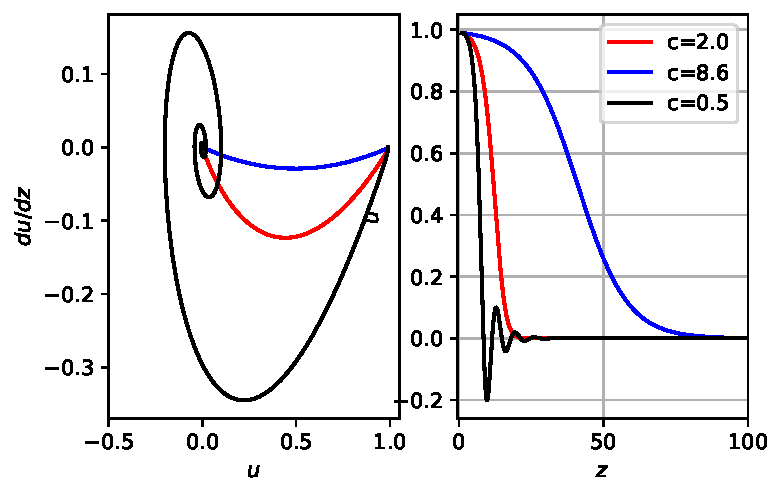
\includegraphics{nonlinearreactiondiffusion_files/figure-pdf/fig-fishernumtravwave-output-1.pdf}

}

\caption{\label{fig-fishernumtravwave}Proposed numerical solution of
Equation~\ref{eq-tw_eq_2} with prospective values of wavespeed \(c\).}

\end{figure}

\hypertarget{steady-state-analysis}{%
\subsection{Steady state analysis}\label{steady-state-analysis}}

The steady states of Equation~\ref{eq-tw_eq_2} are
\((W_1, P_1) = (0,0)\) and \((W_2, P_2) = (1,0)\).

Using \[
\frac{dP}{dW} =  \frac{dP}{dz} \frac{dz}{dW} =\frac{ \frac{dP}{dz}}{ \frac{dW}{dz}}
\] and Equation~\ref{eq-tw_eq_2} we can write an equation for
\(P=P(W)\): \begin{equation}\protect\hypertarget{eq-tw_eq_3}{}{
\frac{ dP}{dW} = - v - \frac{ W(1-W)} P,
}\label{eq-tw_eq_3}\end{equation}

together with \begin{equation}\protect\hypertarget{eq-tw_eq_3_bc}{}{
P(0) = 0, \quad P(1) = 0,
}\label{eq-tw_eq_3_bc}\end{equation} and
\begin{equation}\protect\hypertarget{eq-tw_eq_3_c}{}{
P(W) < 0  \quad \textrm{or} \quad   W \in (0,1). 
}\label{eq-tw_eq_3_c}\end{equation}

The condition Equation~\ref{eq-tw_eq_3_c} is given by the form of
travelling front, which we would like to show that it exists

\begin{lemma}[]\protect\hypertarget{lem-trwave}{}\label{lem-trwave}

For every solution of Equation~\ref{eq-tw_eq} satisfying
Equation~\ref{eq-tw_bc} and Equation~\ref{eq-tw_r} we have that
\(\dfrac{dW(z)}{dz} <0\) for all finite \(z\), i.e.~ \[
P(W) < 0 \quad  \mathrm{for} \quad  W \in (0,1).
\]

\end{lemma}

Thus in phase-plane we shall look for a trajectory connecting
\((W_1, P_1)=(0,0)\) and \((W_2, P_2) = (1,0)\) and \(P<0\).

\hypertarget{connection-between-sign-of-p-and-sign-of-speed-v}{%
\subsection{\texorpdfstring{Connection between sign of \(P\) and sign of
speed
\(v\)}{Connection between sign of P and sign of speed v}}\label{connection-between-sign-of-p-and-sign-of-speed-v}}

Consider Equation~\ref{eq-tw_eq_3}. Multiplying it by \(P\) and
integrating over \(W\) from \(0\) to \(1\), we obtain \[
\int_0^1 \frac{dP}{dW}  P(W)\, dW = - v \int_0^1  P(W) dW - \int_0^1 W(1-W) dW.
\] Using conditions Equation~\ref{eq-tw_eq_3_bc} we have \[
\int_0^1 \frac{dP}{dW} \, P\, dW = \frac 12 \int  \frac{d}{dW} (P^2) dW = \frac 12\left( P^2(1) - P^2(0)\right) = 0,
\] and \[
  v \int_0^1  P(W) dW=  - \int_0^1 W(1-W) dW <0, \quad \text{ since } \int_0^1 W(1-W) dW >0. 
\] Thus for \(v>0\) we have \(P= W^\prime<0\) and for \(v<0\) we have
\(P= W^\prime>0\).

\textbf{Note}: \(u(x,t) = W(z)\), where \(z= x- vt\) with \(v<0\) and
\(\frac{ dW}{dz} >0\) will also be a travelling wave for the Fisher
Equation~\ref{eq-fisher_1}, i.e.~a travelling wave front moving to the
left.

\textbf{Note}: Instead of \(z = x - vt\) we can also consider
\(z=x+ vt\) . The sign of \(v\) determines the direction of movement: If
\(z = x - vt\) \quad for \(v>0\) we have travelling wave moving to the
right and for \(v<0\) we have travelling wave moving to the left.

If \(z = x + vt\) \quad for \(v>0\) we have travelling wave moving to
the left and for \(v<0\) we have travelling wave moving to the right.

\hypertarget{stability-of-steady-states}{%
\subsection{Stability of steady
states}\label{stability-of-steady-states}}

The \textbf{Jacobian matrix} for Equation~\ref{eq-tw_eq_2} is given by:
\[
J(W,P) = \begin{pmatrix}
\frac{\partial F}{\partial W} & \, \frac{\partial F }{\partial P}\\
\frac{\partial G }{\partial W} & \, \frac{\partial G }{\partial P}
\end{pmatrix}  =
\begin{pmatrix}
0 & \,  1\\
-1 + 2W & \, - v 
\end{pmatrix}.
\]

At \((W_1, P_1)=(0,0)\) the eigenvalues of \(J(0,0)\) are solutions of
the characteristic polynomial \[
\det(J(0,0) - \lambda I) = \begin{vmatrix} -\lambda & \, 1\\
- 1 & \, -v - \lambda
\end{vmatrix} = \lambda^2 + v \lambda + 1 = 0.
\] Thus \[
\lambda^{\pm}_1 = \frac 12 ( - v \pm \sqrt{ v^2 - 4})
\] and we have for \(v>0\) that \({R} e(\lambda_1^\pm) <0\).

Therefore at \((0, 0)\) \[
\begin{cases} 
\text{ stable node if }\,   v^2 \geq 4, \\
\text{ stable focus if } \,  v^2 \leq 4 \quad (\text{ complex eigenvalues})
\end{cases}
\] At \((W_2, P_2)=(1,0)\) the eigenvalues of \(J(1,0)\) are solutions
of the characteristic polynomial \[
\det(J(1,0) - \lambda I) = \begin{vmatrix} -\lambda & \, 1 \\
1 & \, -v - \lambda
\end{vmatrix} = \lambda^2 + v \lambda - 1 = 0.
\] Thus \[
\lambda^{\pm}_2 = \frac 12 ( - v \pm \sqrt{ v^2 + 4})
\] and we have for \(v>0\) that \(\lambda_2^{-} <0 < \lambda_2^+\).
Therefore \((1,0)\) is a saddle.

The eigenvectors are defined by \[
- \lambda W + P = 0.
\] Thus at \((W_1, P_1)=(0,0)\) we have \[
\Phi_1 = \begin{pmatrix}
W\\
\lambda_1^- W
\end{pmatrix}, \quad  \Phi_2 = \begin{pmatrix}
W\\
\lambda_1^+ W
\end{pmatrix}. 
\]

Consider that \[
\lambda_1^- \leq \lambda_1^+ <0 \quad \textrm{and choose} \quad W = \pm 1.
\]

At \((W_2, P_2)=(1,0)\) we have \[
\Psi_1 = \begin{pmatrix}
W\\
\lambda_2^- W
\end{pmatrix}, \quad  \Psi_2 = \begin{pmatrix}
W\\
\lambda_2^+ W
\end{pmatrix}.
\]

Consider that \[
\lambda_2^- <0 < \lambda_2^+  \quad \textrm{and choose} \quad W = \pm 1.
\] The eigenvectors are sketched in Figure~\ref{fig-eigenvectors}.

\begin{figure}

{\centering 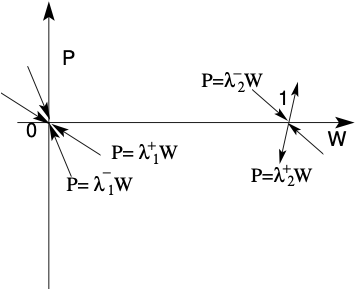
\includegraphics{fig_4.png}

}

\caption{\label{fig-eigenvectors}Schematic diagram of eigenvectors.}

\end{figure}

\begin{definition}[]\protect\hypertarget{def-line}{}\label{def-line}

The trajectory that connects two different points is called a
heteroclinic connection. The trajectory that connects a point with
itself is called a homoclinic connection.

\end{definition}

\hypertarget{minimal-wave-speed}{%
\subsection{Minimal wave speed}\label{minimal-wave-speed}}

It can be shown that for \(v<2\) a heteroclinic connection between
\((0,0)\) and \((1,0)\) exists, but in this situation the steady state
\((0,0)\) is a stable focus and corresponds to an oscillatory front.

In the context of a model of a biological process \(W\) is the profile
of a population density and \(W\geq 0\). Hence, for \(v<2\) trajectories
connecting \((0,0)\) and \((1,0)\) are not biologically realistic.

Thus we obtain the minimal speed \(v^\ast_\text{min}=2\)
(non-dimensionalized) for which we have a travelling wave front solution
for Fisher's equation.

In the original dimensional variables we have: \[
z^\ast= x^\ast - v^\ast t^\ast = x \sqrt{ \frac \rho D} - v^\ast t \rho , \quad 
\sqrt{ \frac D \rho } z^\ast= x  - \sqrt{D \rho}  \, v^\ast\,  t.
\] Thus for \(z = x - vt\) we have \[ 
v=  v^\ast \sqrt{D \rho},
\] and \[
v_{\text{min}}=  v^\ast_{\text{min}} \sqrt{D \rho} = 2  \sqrt{D \rho}.
\]

\hypertarget{the-existence-of-a-confined-region}{%
\subsubsection{The existence of a confined
region}\label{the-existence-of-a-confined-region}}

To show the existence of a travelling wave we will construct a
\textbf{confined region} or \textbf{confined set} in \(\mathbb{R}^2\),
which contains both steady states such that, once inside this region
solution trajectories cannot escape from it (also known as an
\textbf{invariant region} or \textbf{invariant set}).

Consider \[
T= \{ (W,P) : \, 0 \leq W \leq 1,\, \, P \leq 0, \, \,  P \geq \mu W \} 
\] for some \(\mu <0\).

Consider normal vectors at each boundary of \(T\): \[
\text{ at } P = 0 \, : \, \, n_1 = \begin{pmatrix} 
0 \\ -1
\end{pmatrix}, \quad 
\text{ at } W= 1 \, : \, \, n_2 = \begin{pmatrix} 
-1\\ 0
\end{pmatrix}, \quad 
\text{ at } P = \mu W \, : \, \, n_3 = \begin{pmatrix} 
-\mu \\1
\end{pmatrix}.
\] Consider the scalar product between normal vectors and the
\textbf{flow vector} \[
\begin{pmatrix} 
\dfrac{ dW}{dz} \\ \\  \dfrac{dP}{dz}
\end{pmatrix},
\] of Equation~\ref{eq-tw_eq_2}.

At \(P=0\) \[
\begin{pmatrix} 
\dfrac{ dW}{dz} \\  \\ \dfrac{dP}{dz}
\end{pmatrix} \cdot n_1 = \begin{pmatrix} 
\dfrac{ dW}{dz} \\  \\ \dfrac{dP}{dz}
\end{pmatrix}\cdot  \begin{pmatrix} 
0 \\ -1
\end{pmatrix} =  \left(v P + W(1-W)\right) \Big|_{P=0} =  W(1-W) \geq 0 , \text{ for } W\in [0,1].
\]

At \(W=1\) \[
\begin{pmatrix} 
\dfrac{ dW}{dz} \\  \\ \dfrac{dP}{dz}
\end{pmatrix} \cdot n_2 = \begin{pmatrix} 
\dfrac{ dW}{dz} \\  \\ \dfrac{dP}{dz}
\end{pmatrix}\cdot  \begin{pmatrix} 
-1 \\ 0
\end{pmatrix} =  -P  \geq 0 , \text{ since }P \leq 0.
\]

At \(P=\mu W\) \[
\begin{aligned}
\begin{pmatrix} 
\dfrac{ dW}{dz} \\  \\ \dfrac{dP}{dz}
\end{pmatrix} \cdot n_3 &= \begin{pmatrix} 
\dfrac{ dW}{dz} \\  \\ \dfrac{dP}{dz}
\end{pmatrix}\cdot  \begin{pmatrix} 
-\mu \\ 1
\end{pmatrix} \\
& =\left(  - \mu  P - vP -  W(1-W)\right) \Big|_{P=\mu W}  \\
&=   - \mu^2 W - \mu v W - W(1-W) = - W( \mu^2 + \mu v + 1) + W^2.
\end{aligned}
\] Thus

\[
\begin{pmatrix} 
\dfrac{ dW}{dz} \\  \\ \dfrac{dP}{dz}
\end{pmatrix} \cdot n_3 \geq 0,
\] if \[
\mu^2 + \mu v + 1 \leq 0.
\] The last inequality is satisfied if we have real roots of the
equation \(\mu^2 + \mu v + 1 = 0\). We have that

\[
\mu_{1,2} = \frac{ - v \pm \sqrt{ v^2 -4}} 2
\]

are real if \(v^2 \geq 4\).

Thus, since \(v >0\), for \(v \geq 2\) and any \[
\mu\in \left[ \dfrac{ - v -\sqrt{ v^2 -4}} 2, \dfrac{ - v +\sqrt{ v^2 -4}} 2 \right]
\] we have \[
\begin{pmatrix} 
\dfrac{ dW}{dz} \\  \\ \dfrac{dP}{dz}
\end{pmatrix} \cdot n_3 \geq 0 \qquad \text{ at } \quad P=\mu W. 
\]

Therefore we have shown that at the boundaries of \(T\) the flow vector
points in to the region \(T\) and any trajectory approaching the
boundaries from inside of \(T\) will return to \(T\) without crossing
any of the boundaries of \(T\). Thus we have constructed an invariant
(trapping) triangular region containing the steady states \((0,0)\) and
\((1,0)\).

If we can show that there no other steady states or periodic solutions
of the system Equation~\ref{eq-tw_eq_2}, then a trajectory that leaves
\((1,0)\) must approach \((0,0)\).

\begin{theorem}[]\protect\hypertarget{thm-bendixson}{}\label{thm-bendixson}

Bendixson's Negative Criterion, Dulac's Negative Criterion

If there exists a function \(\varphi(W,P)\), with
\(\varphi \in C^1(\mathbb R^2)\), such that \[
 \frac{\partial(\varphi F )}{\partial W} +  \frac{\partial(\varphi G )}{\partial P},
\]

has the same sign \((\neq 0)\) almost everywhere in a simply connected
region (region without holes), then the system \[
 \begin{aligned}
 \dfrac{ dW}{dz} &= F(W,P) \; , 
 \\   \dfrac{dP}{dz} &= G(W,P),
\end{aligned}
\] has no periodic solutions in this region.

\end{theorem}

We can apply Theorem~\ref{thm-bendixson} to our situation taking
\(\varphi(W,P) = 1\). Then using Equation~\ref{eq-tw_eq_2} we have \[
 \frac{\partial(\varphi F )}{\partial W} +  \frac{\partial(\varphi G )}{\partial P} = - v < 0\; .
\] Thus we have no periodic solutions and also only two steady states
\((0,0)\) and \((1,0)\) in the confined (invariant) simply-connected
region \(T\). Therefore the trajectory that leaves \((1,0)\) will
approach \((0,0)\).

We have therefore shown that for any \(v\geq 2\) there exist a
heteroclinic trajectory \(P(W)\) connecting \((0,0)\) and \((1,0)\).

\begin{theorem}[]\protect\hypertarget{thm-trwaveexistence}{}\label{thm-trwaveexistence}

For \(P(W)\) satisfying Equation~\ref{eq-tw_eq_3},
Equation~\ref{eq-tw_eq_3_bc} and \(P(W) < 0\) for \(W \in (0,1)\), there
exists a solution \(W(z)\) of Equation~\ref{eq-tw_eq} satisfying
Equation~\ref{eq-tw_bc} and Equation~\ref{eq-tw_r}.

\end{theorem}

Thus for any wave speed \(v\) satisfying \(v \geq 2\), we have the
existence of travelling wave front \(u(x,t)= W(x- vt)\) of Fisher's
equation Equation~\ref{eq-fisher_1}.

\hypertarget{initial-conditions-1}{%
\subsection{Initial conditions}\label{initial-conditions-1}}

One final key question is: For which initial conditions
\(u(x,0) = u_0(x)\) does the solution evolve to a travelling wave
solution?

If we start with a travelling wave shape initial condition,
i.e.~\(u_0(x)= W(z)|_{t=0} = W(x)\), then this simply propagates as a
travelling wave. However if \(u_0(x)\neq W(x)\), then it is not
immediately obvious how the solution will evolve. This problem was
considered by Kolmogorov et al. Kolmogorov, Petrovsky, and Piskunov
(1937), who showed that for any initial data satisfying \[
 u_0(x) \geq 0, \quad \text{ with} \quad  u_0(x) = \begin{cases} 1 \, \text{ if } \, x \leq x_1, \\
 0 \, \text{ if } \, x \geq x_2, 
 \end{cases}
 \] where \(x_1 < x_2\) and \(u_0\) is continuous in \([x_1, x_2]\), the
solution of Fisher's Equation~\ref{eq-fisher_1} evolves to a travelling
wave with minimal speed \[
 v_\text{ min} = 2 \sqrt{ \rho D}
\] and \[
u(t,x) \rightarrow 1 \quad \textrm{as} \quad x\rightarrow -\infty, \quad u(t,x) \rightarrow 0 \quad \textrm{and} \quad  x\rightarrow +\infty.
\]

\hypertarget{travelling-waves-in-bistable-equations}{%
\section{Travelling waves in bistable
equations}\label{travelling-waves-in-bistable-equations}}

Consider now the reaction-diffusion equation:
\begin{equation}\protect\hypertarget{eq-bistable}{}{
 \frac{\partial u}{\partial t} = \frac{\partial^2 u}{\partial x^2} +   f(u)\qquad x\in \mathbb R, \, \, t >0,  \\
}\label{eq-bistable}\end{equation} with initial condition \[
u(x,0)=u_0(x)  \qquad x\in \mathbb R,
\] where \(f(0) = f(a) = f(1)= 0\) and \(0 < a<1\). There are three
spatially uniform steady states \(u_1 =0\), \(u_2 =a\), \(u_3=1\).

The stability of the steady states is given by the sign of
\(f^\prime(u_j)\) for \(j =1,2,3\).

If we have that \(f^\prime (0) < 0\), \(f^\prime(a) >0\) and
\(f^\prime(1) <0\) then \(u_1=0\) and \(u_3=1\) are stable steady states
and \(u_2 =a\) is an unstable steady state of
Equation~\ref{eq-bistable}.

An example of such a function is \(f\) is \(f=u(u-a)(1-u)\) which arises
in the study of nerve action potentials along nerve fibres and other
problems in \textbf{excitable media}.

The existence of two stable steady states gives rise to the name
``bistable equation'\,'.

\hypertarget{numerical-solutions-2}{%
\section{Numerical solutions}\label{numerical-solutions-2}}

\begin{Shaded}
\begin{Highlighting}[]
\ImportTok{import}\NormalTok{ numpy }\ImportTok{as}\NormalTok{ np}
\ImportTok{from}\NormalTok{ scipy.integrate }\ImportTok{import}\NormalTok{ odeint}
\ImportTok{import}\NormalTok{ matplotlib.pyplot }\ImportTok{as}\NormalTok{ plt}

\NormalTok{T}\OperatorTok{=}\DecValTok{100}
\NormalTok{L}\OperatorTok{=}\DecValTok{100}

\NormalTok{a}\OperatorTok{=}\FloatTok{0.2}

\NormalTok{N\_x}\OperatorTok{=}\DecValTok{100}
\NormalTok{N\_t}\OperatorTok{=}\DecValTok{100}

\NormalTok{t}\OperatorTok{=}\NormalTok{np.linspace(}\DecValTok{1}\NormalTok{,T,N\_t)}
\NormalTok{x}\OperatorTok{=}\NormalTok{np.linspace(}\DecValTok{0}\NormalTok{,L,N\_x)}


\NormalTok{u\_0}\OperatorTok{=}\DecValTok{6}\OperatorTok{*}\FloatTok{0.5}\OperatorTok{*}\NormalTok{(}\DecValTok{1}\OperatorTok{+}\NormalTok{np.tanh(}\OperatorTok{{-}}\DecValTok{1}\OperatorTok{*}\NormalTok{(x}\OperatorTok{{-}}\DecValTok{50}\NormalTok{)))}\OperatorTok{*}\FloatTok{0.5}\OperatorTok{*}\NormalTok{(}\DecValTok{1}\OperatorTok{+}\NormalTok{np.tanh(}\DecValTok{1}\OperatorTok{*}\NormalTok{(x}\OperatorTok{{-}}\DecValTok{50}\NormalTok{)))}
\NormalTok{u\_0}\OperatorTok{=}\FloatTok{0.5}\OperatorTok{*}\NormalTok{(}\DecValTok{1}\OperatorTok{+}\NormalTok{np.tanh(}\OperatorTok{{-}}\DecValTok{1}\OperatorTok{*}\FloatTok{0.2}\OperatorTok{*}\NormalTok{(x}\OperatorTok{{-}}\DecValTok{50}\NormalTok{)))}

\NormalTok{dx}\OperatorTok{=}\NormalTok{L}\OperatorTok{/}\NormalTok{(N\_x}\OperatorTok{{-}}\DecValTok{1}\NormalTok{)}
\NormalTok{dt}\OperatorTok{=}\NormalTok{T}\OperatorTok{/}\NormalTok{(N\_t}\OperatorTok{{-}}\DecValTok{1}\NormalTok{)}

\NormalTok{fig, ax }\OperatorTok{=}\NormalTok{ plt.subplots(}\DecValTok{1}\NormalTok{)}
\NormalTok{u\_samp}\OperatorTok{=}\NormalTok{np.linspace(}\DecValTok{0}\NormalTok{,}\DecValTok{1}\NormalTok{,}\DecValTok{100}\NormalTok{)}
\NormalTok{reac}\OperatorTok{=}\NormalTok{u\_samp}\OperatorTok{*}\NormalTok{(u\_samp}\OperatorTok{{-}}\NormalTok{a)}\OperatorTok{*}\NormalTok{(}\DecValTok{1}\OperatorTok{{-}}\NormalTok{u\_samp)}
\NormalTok{ax.plot(u\_samp,reac) }
\NormalTok{ax.set\_xlabel(}\StringTok{\textquotesingle{}$u$\textquotesingle{}}\NormalTok{)}
\NormalTok{ax.set\_ylabel(}\StringTok{\textquotesingle{}$f(u)$\textquotesingle{}}\NormalTok{)}

\NormalTok{plt.show()}


\KeywordTok{def}\NormalTok{ bistablePDErhs(u,t):}
\NormalTok{    N\_x}\OperatorTok{=}\BuiltInTok{len}\NormalTok{(u)}
\NormalTok{    f}\OperatorTok{=}\NormalTok{np.zeros\_like(u)}
    \ControlFlowTok{for}\NormalTok{ i }\KeywordTok{in} \BuiltInTok{range}\NormalTok{(}\DecValTok{1}\NormalTok{,N\_x}\OperatorTok{{-}}\DecValTok{1}\NormalTok{):}
\NormalTok{      f[i]}\OperatorTok{=}\DecValTok{1}\OperatorTok{/}\NormalTok{dx}\OperatorTok{**}\DecValTok{2}\OperatorTok{*}\NormalTok{(u[i}\OperatorTok{{-}}\DecValTok{1}\NormalTok{]}\OperatorTok{{-}}\DecValTok{2}\OperatorTok{*}\NormalTok{u[i]}\OperatorTok{+}\NormalTok{u[i}\OperatorTok{+}\DecValTok{1}\NormalTok{]) }
\NormalTok{    i}\OperatorTok{=}\DecValTok{0}
\NormalTok{    f[i]}\OperatorTok{=}\DecValTok{1}\OperatorTok{/}\NormalTok{dx}\OperatorTok{**}\DecValTok{2}\OperatorTok{*}\NormalTok{(}\OperatorTok{{-}}\NormalTok{u[i]}\OperatorTok{+}\NormalTok{u[i}\OperatorTok{+}\DecValTok{1}\NormalTok{]) }
\NormalTok{    i}\OperatorTok{=}\NormalTok{N\_x}\OperatorTok{{-}}\DecValTok{1}

\NormalTok{    f[i]}\OperatorTok{=}\DecValTok{1}\OperatorTok{/}\NormalTok{dx}\OperatorTok{**}\DecValTok{2}\OperatorTok{*}\NormalTok{(u[i}\OperatorTok{{-}}\DecValTok{1}\NormalTok{]}\OperatorTok{{-}}\NormalTok{u[i])}

\NormalTok{    reaction}\OperatorTok{=}\NormalTok{u}\OperatorTok{*}\NormalTok{(u}\OperatorTok{{-}}\NormalTok{a)}\OperatorTok{*}\NormalTok{(}\DecValTok{1}\OperatorTok{{-}}\NormalTok{u) }
\NormalTok{    f}\OperatorTok{=}\NormalTok{ f}\OperatorTok{+}\NormalTok{reaction }
    \ControlFlowTok{return}\NormalTok{ f  }

\NormalTok{sol}\OperatorTok{=}\NormalTok{odeint(bistablePDErhs,u\_0,t)}

\NormalTok{plt.plot(x, sol[}\DecValTok{0}\NormalTok{,:], }\StringTok{\textquotesingle{}r\textquotesingle{}}\NormalTok{)}
\NormalTok{plt.plot(x, sol[}\DecValTok{15}\NormalTok{,:], }\StringTok{\textquotesingle{}b\textquotesingle{}}\NormalTok{)}
\NormalTok{plt.plot(x, sol[}\DecValTok{30}\NormalTok{,:], }\StringTok{\textquotesingle{}m\textquotesingle{}}\NormalTok{)}
\NormalTok{plt.plot(x, sol[}\DecValTok{45}\NormalTok{,:], }\StringTok{\textquotesingle{}k\textquotesingle{}}\NormalTok{)}
\NormalTok{plt.legend([}\StringTok{\textquotesingle{}t\textquotesingle{}}\OperatorTok{+} \BuiltInTok{str}\NormalTok{(t[}\DecValTok{0}\NormalTok{]),}\StringTok{\textquotesingle{}t=\textquotesingle{}}\OperatorTok{+} \BuiltInTok{str}\NormalTok{(t[}\DecValTok{4}\NormalTok{]),}\StringTok{\textquotesingle{}t=\textquotesingle{}}\OperatorTok{+} \BuiltInTok{str}\NormalTok{(t[}\DecValTok{8}\NormalTok{]),}\StringTok{\textquotesingle{}t=\textquotesingle{}}\OperatorTok{+} \BuiltInTok{str}\NormalTok{(t[}\DecValTok{12}\NormalTok{])])}
\NormalTok{plt.xlabel(}\StringTok{\textquotesingle{}$x$\textquotesingle{}}\NormalTok{)}
\NormalTok{plt.grid()}
\NormalTok{plt.show()}
\end{Highlighting}
\end{Shaded}

\begin{figure}[H]

{\centering 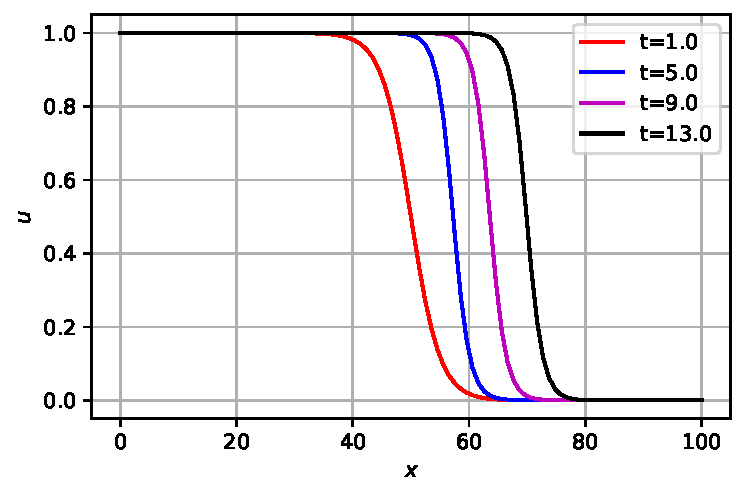
\includegraphics{nonlinearreactiondiffusion_files/figure-pdf/fig-bistablepde-output-1.pdf}

}

\caption{\label{fig-bistablepde}A plot of f(u) against u.}

\end{figure}

\begin{figure}[H]

{\centering 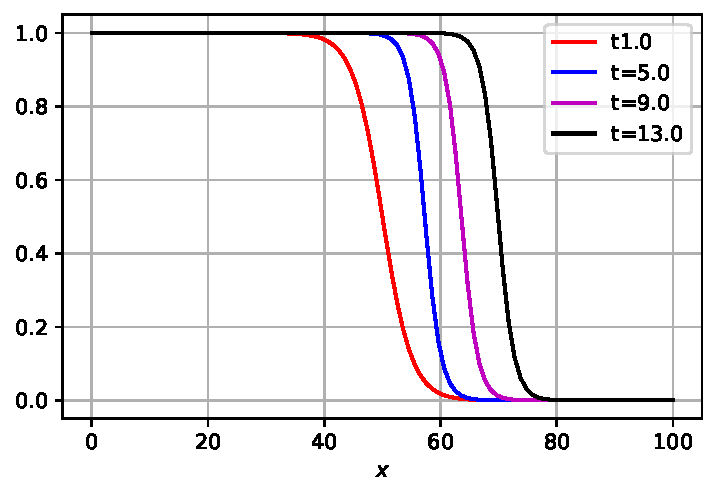
\includegraphics{nonlinearreactiondiffusion_files/figure-pdf/fig-bistablepde-output-2.pdf}

}

\caption{\label{fig-bistablepde}Numerical solution of bistable PDE.}

\end{figure}

\hypertarget{general-assumptions-on-f}{%
\section{\texorpdfstring{General assumptions on
\(f\)}{General assumptions on f}}\label{general-assumptions-on-f}}

\begin{itemize}
\tightlist
\item
  \(f(0)=f(a)=f(1)=0\),
\item
  \(f(u) < 0\) in \((0,a)\), \quad  \(f(u) >0\) in \((a,1)\)
\item
  \(f^\prime (0) < 0\), \quad \(f^\prime (1) < 0\)
\end{itemize}

In a similar manner to the previous sections, we look for a travelling
wave solution of the form \(u(x,t) = W(z)\) with \(z= x-vt\), yielding

\begin{equation}\protect\hypertarget{eq-tw_eq_bis}{}{
 \frac{ d^2W}{dz^2}+  v \frac{ dW}{dz} + f(W)  = 0,  \; .
}\label{eq-tw_eq_bis}\end{equation}

We can rewrite Equation~\ref{eq-tw_eq_bis} as asystem of two 1st order
ODEs \begin{equation}\protect\hypertarget{eq-tw_eq_2_bis}{}{
\begin{aligned}
 \frac{ dW}{dz} = P = F(W,P) , \\
\frac{ d P}{dz}= -  v P - f(W)  = G(W,P),  
\end{aligned}
}\label{eq-tw_eq_2_bis}\end{equation}

\hypertarget{stability-of-the-steady-states}{%
\subsection{Stability of the steady
states}\label{stability-of-the-steady-states}}

The steady states of Equation~\ref{eq-tw_eq_2_bis} are
\((W_1, P_1) = (0,0)\), \((W_2, P_2) = (a,0)\), \((W_3, P_3) = (1,0)\).

The Jacobian matrix is given by \[
J(W,P) = \begin{pmatrix}
\frac{\partial F}{\partial W} & \, \frac{\partial F }{\partial P}\\
\frac{\partial G }{\partial W} & \, \frac{\partial G }{\partial P}
\end{pmatrix}  =
\begin{pmatrix}
0 & \,  1\\
- f^\prime(W) & \, - v 
\end{pmatrix}
\]

At steady states \((W_j, P_j)\), the eigenvalues of \(J(W_j,P_j)\) are
solutions of the characteristic polynomial \[
\det(J(W_j,P_j) - \lambda I) = \begin{vmatrix} -\lambda & \, 1\\
- f^\prime(W_j) & \, -v - \lambda
\end{vmatrix} = \lambda^2 + v \lambda + f^\prime(W_j) = 0 .
\]

Therefore:

\[
 \lambda^{\pm}_j = \frac{ - v \pm \sqrt{ v^2 - 4 f^\prime(W_j)}}2.
\]

At \((W_1, P_1)=(0,0)\) since \(f^\prime(0) <0\) we obtain \$
\lambda\_1\^{}\{-\} \textless0\textless{}\lambda\_1\^{}\{+\} \$ and it
is a saddle point. \textbackslash{}

At \((W_2, P_2)=(a,0)\) since \(f^\prime(a) >0\) we obtain \[
 (a,0) - \begin{cases}
 \text{ focus} \quad \text{ if} \, v^2 < 4 f^\prime(a) \text{ and is stable if } v>0,   \text{ unstable if } v<0, \\
  \text{ node} \quad \text{ if} \, v^2 \geq 4 f^\prime(a) \text{ and is stable if } v>0,   \text{ unstable if } v<0, \\
   \text{centre } \quad \text{ if} \, v=0 \; . \\
 \end{cases}
 \] \textbackslash{} At \((W_3, P_3)=(1,0)\) since \(f^\prime(1) <0\) we
obtain \$ \lambda\_3\^{}\{-\} \textless0\textless{}\lambda\_3\^{}\{+\}
\$ and it is a saddle point. \textbackslash{}

Eigenvectors are given by \[
 P =\lambda W
\] and at each steady state we have two eigenvectors \[
 \Psi_j^{\pm} = \begin{pmatrix}
 W\\
 \lambda_j^\pm W
 \end{pmatrix} , \qquad  j=1,2, 3.
\]

As we vary the wave speed \(v\), the stable and unstable manifolds move
and we wish to show that for some \(v\) the unstable manifold leaving
one saddle point coincides with the stable manifold entering the other
saddle point, i.e.~we can choose a value for the wave speed \(v\) such
that a heteroclinic connection between \((1,0)\) and \((0,0)\) is
obtained. We shall use a ``shooting argument'' to prove this.

\begin{figure}

{\centering 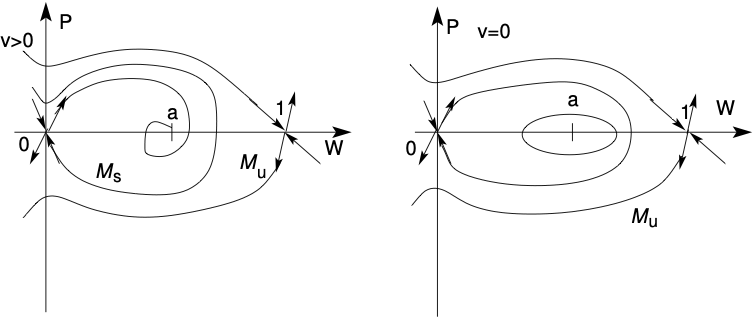
\includegraphics{fig3.png}

}

\caption{\label{fig-eigenvectorsbistable}Schematic diagram of
eigenvectors.}

\end{figure}

\hypertarget{relation-between-sign-of-v-and-sign-of-intlimits_01-fu-du}{%
\subsection{\texorpdfstring{Relation between sign of \(v\) and sign of
\(\int\limits_0^1 f(u) \, du\)}{Relation between sign of v and sign of \textbackslash int\textbackslash limits\_0\^{}1 f(u) \textbackslash, du}}\label{relation-between-sign-of-v-and-sign-of-intlimits_01-fu-du}}

Consider Equation~\ref{eq-tw_eq_bis}, multiply it by \(\dfrac{dW}{dz}\)
and integrate over \((-\infty, + \infty)\): \[
\int_{-\infty}^{+ \infty}  \dfrac{d^2W}{dz^2} \dfrac{dW}{dz} \, dz + v\int_{-\infty}^{+ \infty} \left|\dfrac{dW}{dz} \right|^2\, dz  + \int_{-\infty}^{+ \infty}f(W)\dfrac{dW}{dz} \, dz =0.
\]

Then \[
\frac 12 \int_{-\infty}^{+ \infty}  \dfrac{d}{dz} \left(\left|\dfrac{dW}{dz}\right |^2\right) \, dz + v\int_{-\infty}^{+ \infty} \left|\dfrac{dW}{dz} \right|^2\, dz  + \int_{W(-\infty)}^{W(+\infty)}f(W) \, dW =0
\] and since \(W(z) \to 1\) as \(z \to - \infty\) and \(W(z) \to 0\) as
\(z \to + \infty\) we obtain

\[
\frac 12 \left( \left|\dfrac{dW(+\infty)}{dz}\right |^2-   \left|\dfrac{dW(-\infty)}{dz}\right |^2\right)  + v\int_{-\infty}^{+ \infty} \left|\dfrac{dW}{dz} \right|^2\, dz  + \int_{1}^{0}f(W) \, dW =0.
\] The fact that \(W\) is constant at \(\pm \infty\) implies that \[
\dfrac{dW}{dz}\Big|_{z=-\infty} = \dfrac{dW}{dz}\Big|_{z=+\infty}=0.
\] Thus we have

\[
 v\int\limits_{-\infty}^{+ \infty} \left|\dfrac{dW}{dz} \right|^2\, dz  =  \int\limits_{0}^{1}f(W) dW 
\] and \[
 v= \dfrac {\int\limits_{0}^{1}f(W) \, dW}{\int\limits_{-\infty}^{+ \infty} \left|\dfrac{dW}{dz} \right|^2 dz}.
\] Since
\(\int\limits_{-\infty}^{+ \infty} \left|\dfrac{dW}{dz} \right|^2 dz >0\)
we can conclude that \[
 \int_{0}^{1}f(u) \, du > 0  \quad  \Longrightarrow  \quad v> 0, \\
  \int_{0}^{1}f(u) \, du =0 \quad  \Longrightarrow  \quad v=0, \\
   \int_{0}^{1}f(u) \, du < 0  \quad  \Longrightarrow \quad v < 0. 
\]

\hypertarget{the-shooting-method-proof-of-a-heteroclinic-connection}{%
\subsection{The shooting method proof of a heteroclinic
connection}\label{the-shooting-method-proof-of-a-heteroclinic-connection}}

\hypertarget{numerical-shooting-method}{%
\subsubsection{Numerical shooting
method}\label{numerical-shooting-method}}

\begin{Shaded}
\begin{Highlighting}[]
\ImportTok{import}\NormalTok{ numpy }\ImportTok{as}\NormalTok{ np}
\ImportTok{from}\NormalTok{ scipy.integrate }\ImportTok{import}\NormalTok{ odeint}
\ImportTok{import}\NormalTok{ matplotlib.pyplot }\ImportTok{as}\NormalTok{ plt}

\NormalTok{T}\OperatorTok{=}\DecValTok{300}

\NormalTok{a}\OperatorTok{=}\FloatTok{0.2}
\NormalTok{N\_z}\OperatorTok{=}\DecValTok{5000}

\NormalTok{z}\OperatorTok{=}\NormalTok{np.linspace(}\DecValTok{1}\NormalTok{,T,N\_z)}

\NormalTok{u\_0}\OperatorTok{=}\NormalTok{[}\FloatTok{0.99}\NormalTok{,}\OperatorTok{{-}}\FloatTok{0.0001}\NormalTok{]}

\NormalTok{c\_1}\OperatorTok{=}\FloatTok{2.0}
\NormalTok{c\_2}\OperatorTok{=}\FloatTok{0.6}
\NormalTok{c\_3}\OperatorTok{=}\FloatTok{0.425}

\KeywordTok{def}\NormalTok{ bistableTrWaveODErhs(u, t, c):}
\NormalTok{    f}\OperatorTok{=}\NormalTok{np.zeros\_like(u)}
\NormalTok{    reaction}\OperatorTok{=}\NormalTok{u[}\DecValTok{0}\NormalTok{]}\OperatorTok{*}\NormalTok{(u[}\DecValTok{0}\NormalTok{]}\OperatorTok{{-}}\NormalTok{a)}\OperatorTok{*}\NormalTok{(}\DecValTok{1}\OperatorTok{{-}}\NormalTok{u[}\DecValTok{0}\NormalTok{]) }

\NormalTok{    f[}\DecValTok{0}\NormalTok{]}\OperatorTok{=}\NormalTok{u[}\DecValTok{1}\NormalTok{]}
\NormalTok{    f[}\DecValTok{1}\NormalTok{]}\OperatorTok{={-}}\NormalTok{c}\OperatorTok{*}\NormalTok{u[}\DecValTok{1}\NormalTok{]}\OperatorTok{{-}}\NormalTok{reaction}
    \ControlFlowTok{return}\NormalTok{ f  }

\NormalTok{sol}\OperatorTok{=}\NormalTok{odeint(bistableTrWaveODErhs,u\_0,z, args}\OperatorTok{=}\NormalTok{(c\_1,))}
\NormalTok{sol2}\OperatorTok{=}\NormalTok{odeint(bistableTrWaveODErhs,u\_0,z, args}\OperatorTok{=}\NormalTok{(c\_2,))}
\NormalTok{sol3}\OperatorTok{=}\NormalTok{odeint(bistableTrWaveODErhs,u\_0,z, args}\OperatorTok{=}\NormalTok{(c\_3,))}

\NormalTok{fig, ax }\OperatorTok{=}\NormalTok{ plt.subplots(}\DecValTok{1}\NormalTok{)}
\NormalTok{plt.plot(sol[:,}\DecValTok{0}\NormalTok{],sol[:,}\DecValTok{1}\NormalTok{], }\StringTok{\textquotesingle{}r\textquotesingle{}}\NormalTok{)}
\NormalTok{plt.plot(sol2[:,}\DecValTok{0}\NormalTok{],sol2[:,}\DecValTok{1}\NormalTok{], }\StringTok{\textquotesingle{}b\textquotesingle{}}\NormalTok{)}
\NormalTok{plt.plot(sol3[:,}\DecValTok{0}\NormalTok{],sol3[:,}\DecValTok{1}\NormalTok{], }\StringTok{\textquotesingle{}k\textquotesingle{}}\NormalTok{)}
\NormalTok{ax.set\_xlim([}\OperatorTok{{-}}\FloatTok{0.05}\NormalTok{, }\FloatTok{1.05}\NormalTok{])}

\NormalTok{plt.xlabel(}\StringTok{\textquotesingle{}$u$\textquotesingle{}}\NormalTok{)}
\NormalTok{plt.ylabel(}\StringTok{\textquotesingle{}$du/dz$\textquotesingle{}}\NormalTok{)}
\NormalTok{plt.legend([}\StringTok{\textquotesingle{}c=\textquotesingle{}}\OperatorTok{+}\BuiltInTok{str}\NormalTok{(c\_1),}\StringTok{\textquotesingle{}c=\textquotesingle{}}\OperatorTok{+}\BuiltInTok{str}\NormalTok{(c\_2), }\StringTok{\textquotesingle{}c=\textquotesingle{}}\OperatorTok{+}\BuiltInTok{str}\NormalTok{(c\_3)])}
\NormalTok{plt.grid()}
\NormalTok{plt.show()}
\end{Highlighting}
\end{Shaded}

\begin{figure}[H]

{\centering 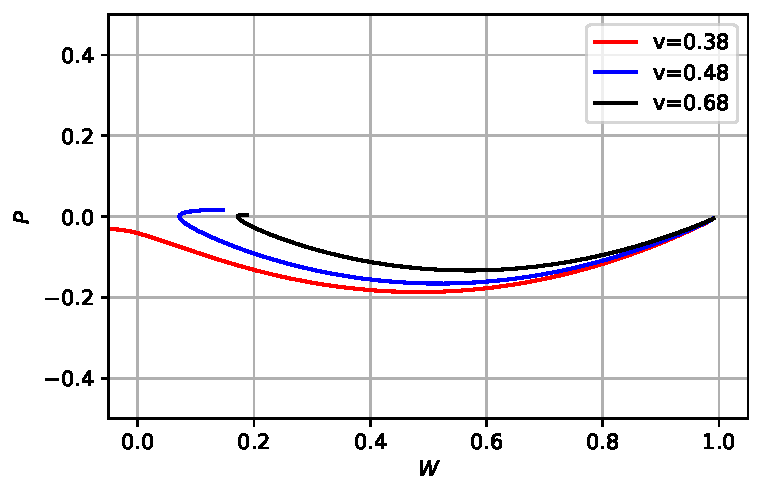
\includegraphics{nonlinearreactiondiffusion_files/figure-pdf/fig-bistablenumtravwave-output-1.pdf}

}

\caption{\label{fig-bistablenumtravwave}Numerical solution of bistable
PDE}

\end{figure}

Assume \[
 \int\limits_{0}^{1}f(u) \, du > 0.
\] i.e.~\(v>0\).

\begin{itemize}
\item
  Consider first \(v=0\).

  From the equations in Equation~\ref{eq-tw_eq_2_bis} and the
  assumptions on the function \(f\) we have

  \begin{itemize}
  \item
    If \(W \in (0,a)\)

    Using the fact that \(f(W) <0\) for \(W \in (0,a)\) and \(P<0\) and
    \(v=0\) we have \[        
      \begin{cases}
      \dfrac{dW}{dz} = P <0, \\
      \dfrac{dP}{dz} = - f(W) >0
      \end{cases}  \quad  \rightarrow \quad \dfrac{dP}{dW} <0
      \] Thus the trajectory enters \((0,0)\) with \[ 
    \dfrac{dP}{dW} <0,
    \] along the stable manifold \(\textit{M}_s^{(0,0)}\) and intersects
    the line \(\{ W=a\}\) at the point \((a, P_0)\).
  \item
    If \(W \in (a,1)\)

    Using the fact that \(f(W) >0\) for \(W \in (a,1)\) and \(P<0\) and
    \(v=0\) we have \[
      \begin{cases}
      \dfrac{dW}{dz} = P <0, \\
      \dfrac{dP}{dz} = - f(W) <0
      \end{cases}  \quad  \rightarrow \quad \dfrac{dP}{dW} >0
      \] Thus the trajectory leaves \((1,0)\) with \[
       \dfrac{dP}{dW} >0
      \] along the unstable manifold \(\textit{M}_u^{(1,0)}\) and
    intersects the line \(\{ W=a\}\) at the point \((a, P_1)\).
  \end{itemize}
\end{itemize}

\begin{figure}

{\centering 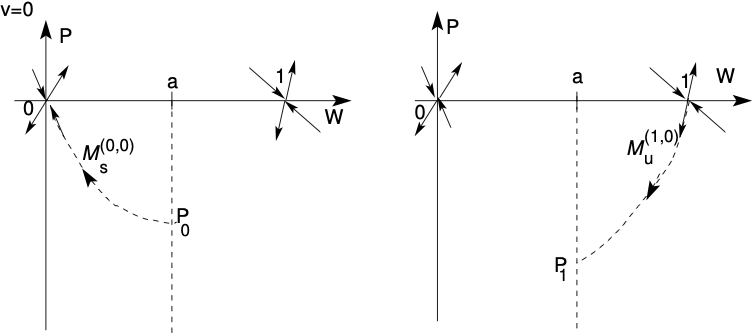
\includegraphics{fig1.png}

}

\caption{\label{fig-shooting}Schematic diagram of eigenvectors.}

\end{figure}

Now we shall compare \(P_0\) and \(P_1\). For this we consider again
equation Equation~\ref{eq-tw_eq_bis}, multiply by \(\dfrac{dW}{dz}\) and
integrate first over \((-\infty, z^\ast)\) and then over
\((z^\ast, + \infty)\), where \(z^\ast \in (-\infty, + \infty)\) such
that \(W(z^\ast)=a\). Then since \(v=0\) we have first \[    
    \int_{-\infty}^{z^\ast}  \dfrac{d^2W}{dz^2} \dfrac{dW}{dz} \, dz   + \int_{-\infty}^{z^\ast}f(W)\dfrac{dW}{dz} \, dz =0.
\] and \[
    \frac 12\left|\dfrac{dW}{dz}\right|^2 \Big|_{z=-\infty}^{z=z^\ast}  + \int_{W(-\infty)}^{W(z^\ast)}f(W) dW=0 \; .
\] Since \(W(-\infty) =1\) we are moving along the unstable manifold
\(M_u^{(1,0)}\) and \[
\dfrac{dW(z^\ast)}{dz}=P(z^\ast+ 0) = P_1.
\] Thus using that \(\dfrac{dW}{dz}\Big|_{z= - \infty} =0\) we obtain

\[
    \frac 12 P^2_1  + \int_{1}^{a}f(W) dW=0 \; \quad  \Longrightarrow \quad  P_1^2 = 2 \int_{a}^{1}f(W) dW
\] Integration over \((z^\ast, + \infty)\) implies \[
\int_{z^\ast}^{+ \infty}  \dfrac{d^2W}{dz^2} \dfrac{dW}{dz} \, dz   + \int_{z^\ast}^{+ \infty} f(W)\dfrac{dW}{dz} \, dz =0.
\] and \[
    \frac 12 \left|\dfrac{dW(+ \infty)}{dz}\right|^2 -  \frac 12 \left|\dfrac{dW(z^\ast)}{dz}\right|^2  + \int_{W(z^\ast)}^{W(+ \infty)} f(W) \, dW =0 \; .
\] Since \(W(+\infty) =0\) we are moving along the stable manifold
\(M_s^{(0,0)}\) and \(\dfrac{dW(z^\ast)}{dz}=P(z^\ast- 0) = P_0\). Thus
using that \(\dfrac{dW}{dz}\Big|_{z= + \infty} =0\) we obtain \[
    -\frac 12 P^2_0  + \int_{a}^{0}f(W) dW=0 \;  \quad  \Longrightarrow \quad  P_0^2 = - 2 \int_{0}^{a}f(W) dW\; .
\] Since \[
\int\limits_{0}^{1}f(u) \, du > 0
\] we obtain \[
P^2_1 - P_0^2=2 \int\limits_{0}^{1}f(W) \, dW > 0   \quad  \Longrightarrow \quad P^2_1 > P_0^2
\] Then since \(P<0\) we have \[
P_1 < P_0 \; .
\]

\begin{itemize}
\tightlist
\item
  Consider \(v>0\) large.
\end{itemize}

From the equations in Equation~\ref{eq-tw_eq_2_bis} and the assumptions
on the function \(f\) we have

\begin{verbatim}
* If $W \in (0,a)$
\end{verbatim}

Using the fact that \(f(W) <0\) for \(W \in (0,a)\), \(P<0\) and \(v>0\)
we have

\[
\begin{aligned}
\begin{cases}
\dfrac{dW}{dz} &= P <0, \\
\dfrac{dP}{dz} &= -vP- f(W) >0
\end{cases}  \quad  \Longrightarrow \quad \dfrac{dP}{dW} <0
\end{aligned}
\] Thus \(P(W)\) is always decreasing for \(W \in (0,a)\). * If
\(W \in (a,1)\)

Using the fact that \(f(W) >0\) for \(W \in (a,1)\), \(P<0\) and \(v>0\)
we have

\[
\begin{aligned}
\dfrac{dW}{dz} = P <0, \\
\\
\begin{cases}
\dfrac{dP}{dz} = -vP- f(W) <0  \quad \text{ for small }  |P| \textrm{ and } 
 \dfrac{dP}{dz} = -vP- f(W) >0  \quad \text{ for large  } |P|.
\end{cases} 
\end{aligned}
\]

Thus \[
\begin{cases}
\dfrac{dP}{dW}   >0 \quad    \text{ for small }  |P| ,\\
\\
\dfrac{dP}{dW}  <0  \quad  \text{ for large }  |P|\; .
\end{cases}
\]

Therefore if \(v>0\) large we have that \(P(W)\) is monotone increasing
for small \(|P|\) and monotone decreasing for large \(|P|\).

\begin{figure}

{\centering 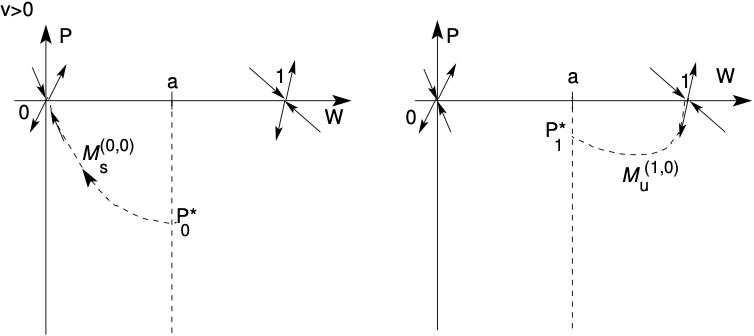
\includegraphics{fig2.png}

}

\caption{\label{fig-2eigenvectors}Schematic diagram.}

\end{figure}

Thus since for \(v=0\) we have \(P_1 < P_0\) and for \(v>0\) we have
that \(P(W)\) is monotone decreasing for large \(|P|\), due to the
continuity of the phase trajectories with respect to the velocity \(v\)
we obtain that there exists a travelling wave speed \(v_0 >0\) such that
\(P_0= P_1\) and we have a heteroclinic connection between \((1,0)\) and
\((0,0)\) in the phase plane. Hence for \(v=v_0\) there exists a
travelling wave front solution for the bistable
Equation~\ref{eq-bistable}.

We can repeat the analysis for \[  
\int\limits_{0}^{1}f(u) \, du < 0
\] and obtain a travelling wave solution with \(v_0 <0\).

If \[
\int\limits_{0}^{1}f(u) \, du = 0,
\] then we have a standing wave with \(v=0\), since the calculations for
\(P_0\) and \(P_1\) implies \(P_0=P_1\) and there exists a heteroclinic
orbit between \((1,0)\) and \((0,0)\) in the phase space.

Note: There exists a unique travelling wave velocity \(v\) for which we
have a travelling wave solution for bistable Equation~\ref{eq-bistable}.

\hypertarget{references}{%
\section{References}\label{references}}

\part{Multi species}

\hypertarget{lotka-voltera-model}{%
\chapter{Lotka Voltera model}\label{lotka-voltera-model}}

Consider a predator-prey system (modified Lotka-Voltera equations) with
diffusion of both the prey and the predator species. Suppose that the
reaction kinetics are given by:

\begin{itemize}
\tightlist
\item
  prey undergoes logistic growth in the absence of predator.
\item
  the predation rate is proportional to the amount of predator
\item
  predator growth rate is proportional to the amount of prey
\item
  predator undergoes natural degradation
\end{itemize}

Suppose also that both predator and prey undero random motion.

Let \(u(x,t)\) and \(n(x,t)\) represent the density of the prey and
predator, respectively. The governing equations are:
\begin{equation}\protect\hypertarget{eq-pp_eq}{}{
\begin{aligned}
\frac{\partial u}{\partial t} &= \rho \, u \left( 1 - \frac u K\right) - \alpha\, u \,  n + D_u \Delta u, \\
\frac{\partial n}{\partial t} &= \beta \; u\, n - \gamma \; n + D_n \Delta n,
\end{aligned} 
}\label{eq-pp_eq}\end{equation}

where

\begin{itemize}
\tightlist
\item
  \(\rho\) -- prey growth rate,
\item
  \(K\) -- carrying capacity,
\item
  \(\beta u\) -- growth rate of the predator,
\item
  \(\alpha\) -- rate at which the predator eats the prey,
\item
  \(\gamma\) -- death rate of the predator,
\item
  \(D_u\) -- diffusion coefficient of the prey
\item
  \(D_n\) - diffusion coefficient for the predator .
\end{itemize}

We will consider one spatial dimension.

\hypertarget{nondimensionalization-1}{%
\section{Nondimensionalization}\label{nondimensionalization-1}}

Consider the scaling \[
 x^\ast = x \sqrt{\frac \rho {D_n}}, \qquad t^\ast = \rho, t , \quad u^\ast = \frac uK, \quad n^\ast = n \frac \alpha \rho.
\] Upon dropping the asteriked notation, Equation~\ref{eq-pp_eq}
transform to \begin{equation}\protect\hypertarget{eq-pp_eq_2}{}{
\begin{cases}
&\dfrac{\partial u}{\partial t} =  u ( 1 - u - n)  + D \dfrac{\partial^2 u}{\partial x^2}\; = \; f(u,n) + D\dfrac{\partial^2 u}{\partial x^2} \qquad x\in \mathbb R , t>0 \,,  \\
& \dfrac{\partial n}{\partial t} = a\,  n(u -b) + \dfrac{\partial^2  n}{\partial x^2}\; =\; \;  g(u,n) + \dfrac{\partial^2  n}{\partial x^2}\;  \qquad x\in \mathbb R , t>0,
\end{cases} 
}\label{eq-pp_eq_2}\end{equation} where \[
D= \dfrac{D_u}{D_n}, \quad a = \dfrac{\beta K}\rho, \quad   b = \dfrac \gamma{ K \beta}.
\]

\hypertarget{numerical-solutions-3}{%
\section{Numerical solutions}\label{numerical-solutions-3}}

In Figure~\ref{fig-lvpde} we plot numerical solution of
Equation~\ref{eq-pp_eq_2}. No flux boundary conditions are imposed at
\(x=0\) and \(x=150\).

\begin{Shaded}
\begin{Highlighting}[]
\ImportTok{import}\NormalTok{ numpy }\ImportTok{as}\NormalTok{ np}
\ImportTok{from}\NormalTok{ scipy.integrate }\ImportTok{import}\NormalTok{ odeint}
\ImportTok{import}\NormalTok{ matplotlib.pyplot }\ImportTok{as}\NormalTok{ plt}

\NormalTok{T}\OperatorTok{=}\DecValTok{100}
\NormalTok{L}\OperatorTok{=}\DecValTok{150}

\NormalTok{a}\OperatorTok{=}\FloatTok{0.2}
\NormalTok{b}\OperatorTok{=}\FloatTok{0.4}
\NormalTok{D\_u}\OperatorTok{=}\FloatTok{0.10}

\NormalTok{N\_x}\OperatorTok{=}\DecValTok{100}
\NormalTok{N\_t}\OperatorTok{=}\DecValTok{100}

\NormalTok{t}\OperatorTok{=}\NormalTok{np.linspace(}\DecValTok{1}\NormalTok{,T,N\_t)}
\NormalTok{x}\OperatorTok{=}\NormalTok{np.linspace(}\DecValTok{0}\NormalTok{,L,N\_x)}

\NormalTok{u\_0}\OperatorTok{=}\NormalTok{b}\OperatorTok{+}\NormalTok{(}\DecValTok{1}\OperatorTok{{-}}\NormalTok{b)}\OperatorTok{*}\FloatTok{0.5}\OperatorTok{*}\NormalTok{(}\DecValTok{1}\OperatorTok{+}\NormalTok{np.tanh(}\DecValTok{1}\OperatorTok{*}\FloatTok{0.5}\OperatorTok{*}\NormalTok{(x}\OperatorTok{{-}}\DecValTok{50}\NormalTok{)))}
\NormalTok{n\_0}\OperatorTok{=}\NormalTok{(}\DecValTok{1}\OperatorTok{{-}}\NormalTok{b)}\OperatorTok{*}\FloatTok{0.5}\OperatorTok{*}\NormalTok{(}\DecValTok{1}\OperatorTok{+}\NormalTok{np.tanh(}\OperatorTok{{-}}\DecValTok{1}\OperatorTok{*}\FloatTok{0.5}\OperatorTok{*}\NormalTok{(x}\OperatorTok{{-}}\DecValTok{50}\NormalTok{)))}

\NormalTok{u\_0}\OperatorTok{=}\NormalTok{np.concatenate((u\_0,n\_0))}

\NormalTok{dx}\OperatorTok{=}\NormalTok{L}\OperatorTok{/}\NormalTok{(N\_x}\OperatorTok{{-}}\DecValTok{1}\NormalTok{)}
\NormalTok{dt}\OperatorTok{=}\NormalTok{T}\OperatorTok{/}\NormalTok{(N\_t}\OperatorTok{{-}}\DecValTok{1}\NormalTok{)}

\KeywordTok{def}\NormalTok{ LVPDErhs(sol,t):}

\NormalTok{    N\_x}\OperatorTok{=}\BuiltInTok{int}\NormalTok{(np.ceil(}\BuiltInTok{len}\NormalTok{(sol)}\OperatorTok{/}\DecValTok{2}\NormalTok{))}

\NormalTok{    u}\OperatorTok{=}\NormalTok{sol[}\DecValTok{0}\NormalTok{:N\_x]}
\NormalTok{    n}\OperatorTok{=}\NormalTok{sol[N\_x:}\DecValTok{2}\OperatorTok{*}\NormalTok{N\_x]}



\NormalTok{    f\_u}\OperatorTok{=}\NormalTok{np.zeros\_like(u)}
\NormalTok{    f\_n}\OperatorTok{=}\NormalTok{np.zeros\_like(u)}

    \ControlFlowTok{for}\NormalTok{ i }\KeywordTok{in} \BuiltInTok{range}\NormalTok{(}\DecValTok{1}\NormalTok{,N\_x}\OperatorTok{{-}}\DecValTok{2}\NormalTok{):}
\NormalTok{      f\_u[i]}\OperatorTok{=}\NormalTok{D\_u}\OperatorTok{/}\NormalTok{dx}\OperatorTok{**}\DecValTok{2}\OperatorTok{*}\NormalTok{(u[i}\OperatorTok{{-}}\DecValTok{1}\NormalTok{]}\OperatorTok{{-}}\DecValTok{2}\OperatorTok{*}\NormalTok{u[i]}\OperatorTok{+}\NormalTok{u[i}\OperatorTok{+}\DecValTok{1}\NormalTok{]) }
\NormalTok{    i}\OperatorTok{=}\DecValTok{0}
\NormalTok{    f\_u[i]}\OperatorTok{=}\NormalTok{D\_u}\OperatorTok{/}\NormalTok{dx}\OperatorTok{**}\DecValTok{2}\OperatorTok{*}\NormalTok{(}\OperatorTok{{-}}\NormalTok{u[i]}\OperatorTok{+}\NormalTok{u[i}\OperatorTok{+}\DecValTok{1}\NormalTok{]) }
\NormalTok{    i}\OperatorTok{=}\NormalTok{N\_x}\OperatorTok{{-}}\DecValTok{1}
\NormalTok{    f\_u[i]}\OperatorTok{=}\NormalTok{D\_u}\OperatorTok{/}\NormalTok{dx}\OperatorTok{**}\DecValTok{2}\OperatorTok{*}\NormalTok{(u[i}\OperatorTok{{-}}\DecValTok{1}\NormalTok{]}\OperatorTok{{-}}\NormalTok{u[i])}

    \ControlFlowTok{for}\NormalTok{ i }\KeywordTok{in} \BuiltInTok{range}\NormalTok{(}\DecValTok{1}\NormalTok{,N\_x}\OperatorTok{{-}}\DecValTok{2}\NormalTok{):}
\NormalTok{      f\_n[i]}\OperatorTok{=}\DecValTok{1}\OperatorTok{/}\NormalTok{dx}\OperatorTok{**}\DecValTok{2}\OperatorTok{*}\NormalTok{(n[i}\OperatorTok{{-}}\DecValTok{1}\NormalTok{]}\OperatorTok{{-}}\DecValTok{2}\OperatorTok{*}\NormalTok{n[i]}\OperatorTok{+}\NormalTok{n[i}\OperatorTok{+}\DecValTok{1}\NormalTok{]) }
\NormalTok{    i}\OperatorTok{=}\DecValTok{0}
\NormalTok{    f\_n[i]}\OperatorTok{=}\DecValTok{1}\OperatorTok{/}\NormalTok{dx}\OperatorTok{**}\DecValTok{2}\OperatorTok{*}\NormalTok{(}\OperatorTok{{-}}\NormalTok{n[i]}\OperatorTok{+}\NormalTok{n[i}\OperatorTok{+}\DecValTok{1}\NormalTok{]) }
\NormalTok{    i}\OperatorTok{=}\NormalTok{N\_x}\OperatorTok{{-}}\DecValTok{1}
\NormalTok{    f\_n[i]}\OperatorTok{=}\DecValTok{1}\OperatorTok{/}\NormalTok{dx}\OperatorTok{**}\DecValTok{2}\OperatorTok{*}\NormalTok{(n[i}\OperatorTok{{-}}\DecValTok{1}\NormalTok{]}\OperatorTok{{-}}\NormalTok{n[i])}

\NormalTok{    reaction\_u}\OperatorTok{=}\NormalTok{u}\OperatorTok{*}\NormalTok{(}\DecValTok{1}\OperatorTok{{-}}\NormalTok{u}\OperatorTok{{-}}\NormalTok{n)}
\NormalTok{    reaction\_n}\OperatorTok{=}\NormalTok{a}\OperatorTok{*}\NormalTok{n}\OperatorTok{*}\NormalTok{(u}\OperatorTok{{-}}\NormalTok{b)}

\NormalTok{    f\_u}\OperatorTok{=}\NormalTok{f\_u}\OperatorTok{+}\NormalTok{reaction\_u}
\NormalTok{    f\_n}\OperatorTok{=}\NormalTok{f\_n}\OperatorTok{+}\NormalTok{reaction\_n}

\NormalTok{    f}\OperatorTok{=}\NormalTok{ np.concatenate((f\_u, f\_n)) }
    \ControlFlowTok{return}\NormalTok{ f  }

\NormalTok{sol}\OperatorTok{=}\NormalTok{odeint(LVPDErhs,u\_0,t)}

\NormalTok{u}\OperatorTok{=}\NormalTok{sol[:,}\DecValTok{0}\NormalTok{:N\_x]}
\NormalTok{n}\OperatorTok{=}\NormalTok{sol[:,N\_x:}\DecValTok{2}\OperatorTok{*}\NormalTok{N\_x]}

\NormalTok{fig, ax }\OperatorTok{=}\NormalTok{ plt.subplots(}\DecValTok{2}\NormalTok{,}\DecValTok{1}\NormalTok{)}

\NormalTok{ax[}\DecValTok{0}\NormalTok{].plot(x,u[}\DecValTok{0}\NormalTok{,:],}\StringTok{\textquotesingle{}r\textquotesingle{}}\NormalTok{)}
\NormalTok{ax[}\DecValTok{0}\NormalTok{].plot(x,u[}\DecValTok{16}\NormalTok{,:],}\StringTok{\textquotesingle{}b\textquotesingle{}}\NormalTok{)}
\NormalTok{ax[}\DecValTok{0}\NormalTok{].plot(x,u[}\DecValTok{32}\NormalTok{,:],}\StringTok{\textquotesingle{}m\textquotesingle{}}\NormalTok{)}
\NormalTok{ax[}\DecValTok{0}\NormalTok{].plot(x,u[}\DecValTok{48}\NormalTok{,:],}\StringTok{\textquotesingle{}k\textquotesingle{}}\NormalTok{)}
\NormalTok{ax[}\DecValTok{0}\NormalTok{].set\_xlabel(}\StringTok{\textquotesingle{}$x$\textquotesingle{}}\NormalTok{)}
\NormalTok{ax[}\DecValTok{0}\NormalTok{].set\_ylabel(}\StringTok{\textquotesingle{}$u$\textquotesingle{}}\NormalTok{)}

\NormalTok{ax[}\DecValTok{1}\NormalTok{].plot(x, n[}\DecValTok{0}\NormalTok{,:],}\StringTok{\textquotesingle{}r{-}{-}\textquotesingle{}}\NormalTok{)}
\NormalTok{ax[}\DecValTok{1}\NormalTok{].plot(x, n[}\DecValTok{16}\NormalTok{,:],}\StringTok{\textquotesingle{}b{-}{-}\textquotesingle{}}\NormalTok{)}
\NormalTok{ax[}\DecValTok{1}\NormalTok{].plot(x, n[}\DecValTok{32}\NormalTok{,:],}\StringTok{\textquotesingle{}m{-}{-}\textquotesingle{}}\NormalTok{)}
\NormalTok{ax[}\DecValTok{1}\NormalTok{].plot(x, n[}\DecValTok{48}\NormalTok{,:],}\StringTok{\textquotesingle{}k{-}{-}\textquotesingle{}}\NormalTok{)}
\NormalTok{ax[}\DecValTok{1}\NormalTok{].set\_xlabel(}\StringTok{\textquotesingle{}$x$\textquotesingle{}}\NormalTok{)}
\NormalTok{ax[}\DecValTok{1}\NormalTok{].set\_ylabel(}\StringTok{\textquotesingle{}$n$\textquotesingle{}}\NormalTok{)}

\NormalTok{plt.legend([}\StringTok{\textquotesingle{}t\textquotesingle{}}\OperatorTok{+} \BuiltInTok{str}\NormalTok{(t[}\DecValTok{0}\NormalTok{]),}\StringTok{\textquotesingle{}t=\textquotesingle{}}\OperatorTok{+} \BuiltInTok{str}\NormalTok{(t[}\DecValTok{4}\NormalTok{]),}\StringTok{\textquotesingle{}t=\textquotesingle{}}\OperatorTok{+} \BuiltInTok{str}\NormalTok{(t[}\DecValTok{8}\NormalTok{]),}\StringTok{\textquotesingle{}t=\textquotesingle{}}\OperatorTok{+} \BuiltInTok{str}\NormalTok{(t[}\DecValTok{12}\NormalTok{])])}
\NormalTok{plt.xlabel(}\StringTok{\textquotesingle{}$x$\textquotesingle{}}\NormalTok{)}
\NormalTok{plt.grid()}
\NormalTok{plt.show()}
\end{Highlighting}
\end{Shaded}

\begin{figure}[H]

{\centering 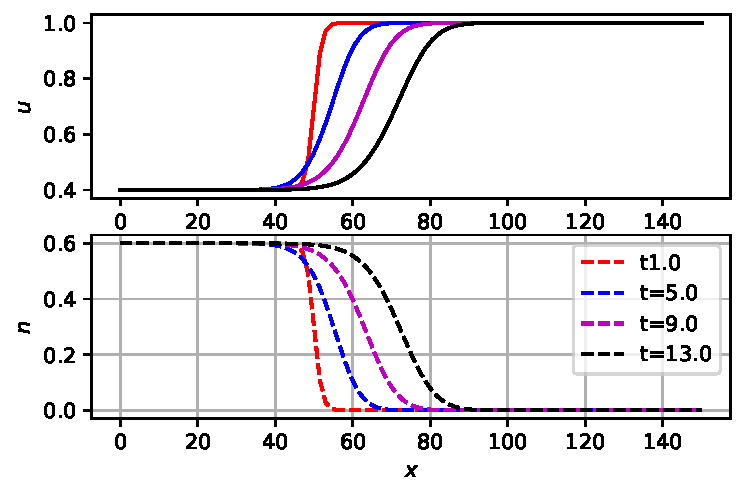
\includegraphics{LotkaVolteraPDE_files/figure-pdf/fig-lvpde-output-1.pdf}

}

\caption{\label{fig-lvpde}Numerical solution of LV model. \(a\)=0.2.
\(b\)=0.4.}

\end{figure}

\hypertarget{spatially-homogeneous-steady-states}{%
\section{Spatially homogeneous steady
states}\label{spatially-homogeneous-steady-states}}

We firstly consider spatially homogeneous steady states, i.e. \[
f(u,n) =0, \quad g(u,n) = 0.
\] Thus \[
\begin{aligned}
 &u(1-u-n) = 0,  \quad  u =0, \quad u+n=1,\\
 & an(u-b) = 0,  \quad n =0, \quad u =b.
 \end{aligned}
\] Thus the steady states are \[
 (u_1^\ast, n_1^\ast)= (0,0), \quad (u_2^\ast, n_2^\ast)= (1,0), \quad (u_3^\ast, n_3^\ast)= (b,1-b), \, 0\leq b <1.
\]

\hypertarget{stability-of-steady-states-to-spatially-homogeneous-perturbations}{%
\section{Stability of steady states to spatially homogeneous
perturbations}\label{stability-of-steady-states-to-spatially-homogeneous-perturbations}}

The Jacobian matrix is \[
\begin{aligned}
J(u_j^\ast, n^\ast_j) = 
\begin{pmatrix}
1-2u -n & -u \\
an &a(u-b)
\end{pmatrix}_{(u^\ast_j, n^\ast_j)}, \quad j = 1,2,3.
\end{aligned}
\]

For \[
(u_1^\ast, n_1^\ast)= (0,0)
\]

\[
\det(J (0,0) - \lambda I) = - (1- \lambda)(\lambda+ ab) = 0
\]

and \[
\lambda_1^+ = 1, \quad \lambda_1^- = - ab <0.
\]

Thus \((0,0)\) is a saddle point.

For \[
(u_2^\ast, n_2^\ast)= (1,0)
\]

\[
\det(J (1,0) - \lambda I) = - (1+ \lambda)(a(1-b)- \lambda) = 0
\] and \[
\lambda_2^- =- 1, \quad \lambda_2^+ = a(1-b) >0 \; \text{ for } \; 0 \leq b <1.
\]

Thus \((1,0)\) is a saddle point.

For \((u_3^\ast, n_3^\ast)= (b,1-b)\) \[
\det(J (b,1-b) - \lambda I) =\lambda^2 + b \lambda + ab(1-b) = 0.
\]

If \[
4 ab (1-b) \leq b^2  \implies \lambda_3^{\pm} < 0. 
\] Hence (\(b,1-b\)) is a stable node.

If\\
\[
4 ab (1-b) > b^2 \qquad \implies  \Re(\lambda_3{\pm}) < 0,  \Im(\lambda_3^{\pm}) \neq 0.
\] Hence (\(b,1-b\)) is a stable focus (spiral).

For \(b>0\), \(1-b>0\) spiral oscillations are biologically realistic so
long \(u>0\) and \(n>0\).

\hypertarget{existence-of-travelling-wave-profiles-connection-10-and-b1-b}{%
\section{\texorpdfstring{Existence of travelling wave profiles
connection \((1,0)\) and
\((b,1-b)\)}{Existence of travelling wave profiles connection (1,0) and (b,1-b)}}\label{existence-of-travelling-wave-profiles-connection-10-and-b1-b}}

We make travelling wave \emph{ansatz} \[
\begin{aligned}
u(t,x) &= W(x+ vt) = W(z), \quad v>0, \\
n(t,x) &= N( x + vt) = N(z), \quad v >0,
\end{aligned}
\]

in Equation~\ref{eq-pp_eq_2} and consider the boundary conditions \[
\begin{aligned}
u(t,x) \to 1 \; \text{ as } x \to - \infty,  & \; \qquad  W(z)\to 1 \; \text{ as } z \to - \infty, \quad\\
 u(t,x) \to b \; \text{ as } x \to +\infty, & \;  \qquad   W(z)\to b \; \text{ as } z \to + \infty, \\
n(t,x) \to 0 \;  \text{ as } x \to - \infty ,  &\qquad  \;  N(z)\to 0 \;  \text{ as } z \to - \infty, \quad \\
n(t,x) \to 1-b \; \text{ as } x \to +\infty, & \;  \qquad N(z)\to 1-b \;  \text{ as } z \to +\infty.
\end{aligned}
\]

The system Equation~\ref{eq-pp_eq_2} transforms to \[
\begin{aligned}
v \frac{dW}{dz} &= D \frac{d^2W}{dz^2} + W(1-W-N),\\
v \frac{dN}{dz} &=  \frac{d^2N}{dz^2} + a N(W-b), 
\end{aligned}
\]

with boundary conditions given by
\begin{equation}\protect\hypertarget{eq-tw_pp}{}{
\begin{aligned}
& W(z)\to 1 \; \text{ as } z \to - \infty, \quad W(z)\to b \; \text{ as } z \to + \infty, \\
 & N(z)\to 0 \;  \text{ as } z \to - \infty, \quad N(z)\to 1-b \;  \text{ as } z \to +\infty.
  \end{aligned}
}\label{eq-tw_pp}\end{equation}

Upon making the assumption that the prey moves much more slowly than the
predator species, i.e.~ \[
D= D_u/D_n \ll 1,
\]

Equation~\ref{eq-tw_pp} simplify to

\begin{equation}\protect\hypertarget{eq-tw_pp_2}{}{
\begin{aligned}
v \frac{dW}{dz} &=  W(1-W-N) ,\\
v \frac{dN}{dz} &=  \frac{d^2N}{dz^2} + a N(W-b). 
\end{aligned}
}\label{eq-tw_pp_2}\end{equation}

We can rewrite Equation~\ref{eq-tw_pp_2} as a system of first order
ODEs: \begin{equation}\protect\hypertarget{eq-tw_pp_3}{}{
\begin{aligned}
\frac{dW}{dz} &= \frac 1 v W(1-W-N) = F(W,N,P),\\
\frac{dN}{dz} &= P  = G(W, N,P),\\
\frac{dP}{dz} &= v P - a N(W-b)  = R(W,N,P). 
\end{aligned}
}\label{eq-tw_pp_3}\end{equation}

The steady states of Equation~\ref{eq-tw_pp_3} are \[
\begin{aligned}
(W^\ast_1, N^\ast_1, P^\ast_1) &= (0,0,0),\\
(W^\ast_2, N^\ast_2, P^\ast_2) &= (1,0,0), \\
(W^\ast_3, N^\ast_3, P^\ast_3) &=(b, 1-b, 0).
\end{aligned}
\]

The Jacobian matrix is \[
J(W,N,P) = \begin{pmatrix}
\dfrac 1 v - \dfrac{2W} v - \dfrac Nv & - \dfrac Wv & 0 \\
0 & 0 & 1 \\
- aN & a(b-W) & v 
\end{pmatrix}.
\]

At \[
(W^\ast_1, N^\ast_1, P^\ast_1) = (0,0,0)
\]

we have \[
\det(J(0,0,0) - \lambda I)= \left( \frac 1 v - \lambda\right) (\lambda^2 - \lambda v - ab) =0
\] and \[
\lambda_1^1= \frac 1 v > 0, \quad \lambda_2^{\pm} = \frac{ v \pm \sqrt{v^2 + 4 ab} } 2
\]

Thus \((0,0,0)\) is a saddle point with a \(2\)-dim unstable manifold

At \((W^\ast_2, N^\ast_2, P^\ast_2) = (1,0,0)\) we have \[
\det(J(1,0,0) - \lambda I)= \left(- \frac 1 v - \lambda\right) (\lambda^2 - \lambda v + a(1-b)) =0
\]

and \[
\lambda_1^1= -\frac 1 v < 0, \quad \lambda_2^{\pm} = \frac{ v \pm \sqrt{v^2 - 4 a(1-b)} } 2
\]

Thus since, \(0\leq b < 1\) and \(4(1-b)>0\), \[
\begin{aligned}
\text{If } &&  v^2 \geq  4 a(1-b) \quad (1,0,0) \text{ is a saddle with 2-dim unstable manifold},\\
 \text{If } &&  v^2 <  4 a(1-b) \quad (1,0,0) \text{ is an unstable focus}
\end{aligned}
\]

Thus for a travelling wave with \(W\geq 0\) and \(N \geq 0\) to exist we
require \[
v^2 \geq  4 a(1-b)
\]

and obtain a minimal wave speed \[
v_\text{min}=2\sqrt{a(1-b)}   \quad \text{ with } \quad  0\leq b<1.
\]

At \((W^\ast_3, N^\ast_3, P^\ast_3) =(b, 1-b, 0)\) we have \[
\det(J(b,1-b,0) - \lambda I)= \lambda^3 - \lambda^2(v- \frac b v) - \lambda b - \frac 1 v ab(1-b) = p(\lambda) =0.
\]

It can be shown that the extrema of \(p(\lambda)\) are independent of
the parameter \(a\).

To identify extrema, we compute \[
p^\prime(\lambda) = 3 \lambda^2 - 2 \lambda \left( v - \frac b v\right) - b = 0
\]

and find that \[
\lambda_{m,M}= \frac 13 \left[ \left(v - \frac bv \right) \pm \sqrt{ \left(v - \frac bv\right) ^2 + 3 b } \right].
\]

If \(a=0\), the eigenvalues are \[
\lambda_3^1 = 0, \quad \lambda_3^\pm = \frac 12 \left( v - \frac bv \pm \sqrt{\left(v - \frac bv\right)^2 + 4 b} \right).
\]

Thus there exists a critical value \(a^\ast>0\) such that for
\(a \in (0, a^\ast)\) we obtain \(2\) real negative eigenvalues and
\(1\) positive real eigenvalue and \((b, 1-b, 0)\) is a saddle with
\(2\)-dim stable manifold and \(1\)-dim unstable manifold

For \(a>a^\ast\) we will have a pair of complex conjugate eigenvalues
with negative real part and one real positive eigenvalue corresponding
to \(1\)-dim unstable manifold.

This can be easily seen from a sketch of the cubic equation:

\[
p(\lambda) = \lambda^3 - \lambda^2(v- \frac b v) - \lambda b - \frac 1 v ab(1-b).
\]

\begin{figure}

{\centering 

\begin{Shaded}
\begin{Highlighting}[]
\ImportTok{import}\NormalTok{ numpy }\ImportTok{as}\NormalTok{ np}
\ImportTok{import}\NormalTok{ matplotlib.pyplot }\ImportTok{as}\NormalTok{ plt}

\NormalTok{lam}\OperatorTok{=}\NormalTok{np.linspace(}\OperatorTok{{-}}\FloatTok{1.2}\NormalTok{,}\FloatTok{1.2}\NormalTok{,}\DecValTok{100}\NormalTok{)}
\NormalTok{a}\OperatorTok{=}\FloatTok{0.0}
\NormalTok{a2}\OperatorTok{=}\FloatTok{0.05}
\NormalTok{a3}\OperatorTok{=}\FloatTok{0.2}
\NormalTok{b}\OperatorTok{=}\FloatTok{0.2}
\NormalTok{v}\OperatorTok{=}\FloatTok{0.5}

\NormalTok{p1}\OperatorTok{=}\NormalTok{ lam}\OperatorTok{**}\DecValTok{3}\OperatorTok{{-}}\NormalTok{lam}\OperatorTok{**}\DecValTok{2}\OperatorTok{*}\NormalTok{(v}\OperatorTok{{-}}\NormalTok{b}\OperatorTok{/}\NormalTok{v)}\OperatorTok{{-}}\NormalTok{lam}\OperatorTok{*}\NormalTok{b}\OperatorTok{{-}}\DecValTok{1}\OperatorTok{/}\NormalTok{v}\OperatorTok{*}\NormalTok{a}\OperatorTok{*}\NormalTok{b}\OperatorTok{*}\NormalTok{(}\DecValTok{1}\OperatorTok{{-}}\NormalTok{b)}
\NormalTok{p2}\OperatorTok{=}\NormalTok{ lam}\OperatorTok{**}\DecValTok{3}\OperatorTok{{-}}\NormalTok{lam}\OperatorTok{**}\DecValTok{2}\OperatorTok{*}\NormalTok{(v}\OperatorTok{{-}}\NormalTok{b}\OperatorTok{/}\NormalTok{v)}\OperatorTok{{-}}\NormalTok{lam}\OperatorTok{*}\NormalTok{b}\OperatorTok{{-}}\DecValTok{1}\OperatorTok{/}\NormalTok{v}\OperatorTok{*}\NormalTok{a2}\OperatorTok{*}\NormalTok{b}\OperatorTok{*}\NormalTok{(}\DecValTok{1}\OperatorTok{{-}}\NormalTok{b)}
\NormalTok{p3}\OperatorTok{=}\NormalTok{ lam}\OperatorTok{**}\DecValTok{3}\OperatorTok{{-}}\NormalTok{lam}\OperatorTok{**}\DecValTok{2}\OperatorTok{*}\NormalTok{(v}\OperatorTok{{-}}\NormalTok{b}\OperatorTok{/}\NormalTok{v)}\OperatorTok{{-}}\NormalTok{lam}\OperatorTok{*}\NormalTok{b}\OperatorTok{{-}}\DecValTok{1}\OperatorTok{/}\NormalTok{v}\OperatorTok{*}\NormalTok{a3}\OperatorTok{*}\NormalTok{b}\OperatorTok{*}\NormalTok{(}\DecValTok{1}\OperatorTok{{-}}\NormalTok{b)}

\NormalTok{fig, ax}\OperatorTok{=}\NormalTok{ plt.subplots()}
\NormalTok{ax.plot(lam,p1,lam,p2,lam,p3)}
\NormalTok{ax.grid(}\VariableTok{True}\NormalTok{)}
\NormalTok{ax.set\_ylim([}\OperatorTok{{-}}\FloatTok{0.5}\NormalTok{, }\FloatTok{0.5}\NormalTok{])}
\end{Highlighting}
\end{Shaded}

\begin{figure}

{\centering 

\begin{verbatim}
(-0.5, 0.5)
\end{verbatim}

}

\caption{Plot of cubic.}

\end{figure}

\begin{figure}[H]

{\centering 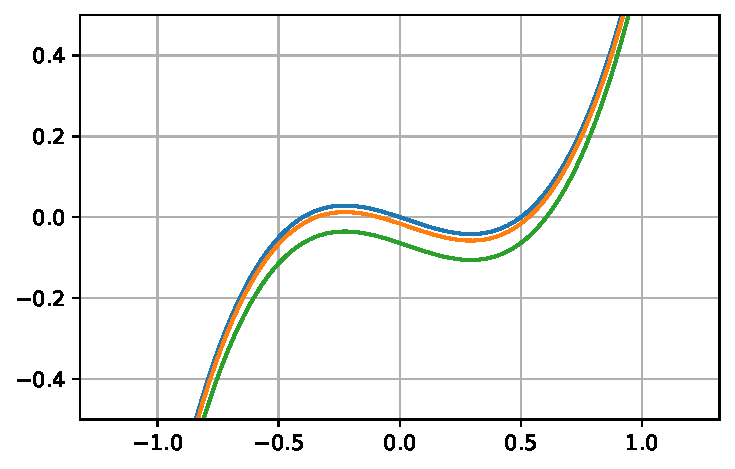
\includegraphics{LotkaVolteraPDE_files/figure-pdf/fig-cubic-output-2.pdf}

}

\end{figure}

}

\caption{\label{fig-cubic}\textbf{?(caption)}}

\end{figure}

Thus we have a possible heteroclinic connection between \((1,0,0)\) and
\((b, 1-b, 0)\), i.e.~between \(2\)-dim unstable manifold at \((1,0,0)\)
and \(2\)-dim stable manifold at \((b, 1-b, 0)\), and therefore an
existence of a travelling wave front solution for
Equation~\ref{eq-pp_eq_2} with

\[
\begin{aligned}
u(x,t) \to 1 \; \text{ as } x \to - \infty,  \quad & u(x,t) \to b \; \text{ as } x \to +\infty,  \\
n(x,t) \to 0 \;  \text{ as } x \to - \infty ,  \quad & n(x,t) \to 1-b \; \text{ as } x \to +\infty.
\end{aligned}
\]

\hypertarget{exercise}{%
\section{Exercise}\label{exercise}}

Use Python code to numerically investigate dependence of travelling wave
solution on the parameter \(a\).

\hypertarget{aggregation-via-chemotaxis}{%
\chapter{Aggregation via Chemotaxis}\label{aggregation-via-chemotaxis}}

\textbf{Dictyostelium discoideum} (Dicty) is a slime-mold that is widely
studied experimentally as a model organism. The individual amoebae that
constitute a slime-mold exhibit a range of phenomena also observed in
mammalian cells e.g.~differentiation, proliferation, migration.

Under nutirent starvation conditions, Dicty cells undergo complex
collective behaviours. Individual amoebae secrete a diffusible chemical,
cyclic AMP or cAMP. The amoebae respond chemotactically to cAMP and
begin to migrate towards regions of high cAMP concentration via
\emph{chemotaxis}. As they migrate they generate a range of intricate
patterns including \emph{spiral waves} and \emph{streaming} aggregation
patterns (e.g. Figure~\ref{fig-dicty_spiral}).

See also \href{https://www.youtube.com/watch?v=bkVhLJLG7ug}{this link to
a fascinating Youtube movie of slime mold aggregation}. Note the
aggregation between 0:35 and 0.48.

\url{https://www.youtube.com/watch?v=bkVhLJLG7ug}

In Figure~\ref{fig-dicty_spiral} we can see stills-shot images of spiral
patterns. This spirals are dynamic as can be seen
\href{https://www.youtube.com/watch?v=OX5Yiz38fgY}{in this movie}. See
spiral pattern at around 0:36.

\begin{figure}

{\centering 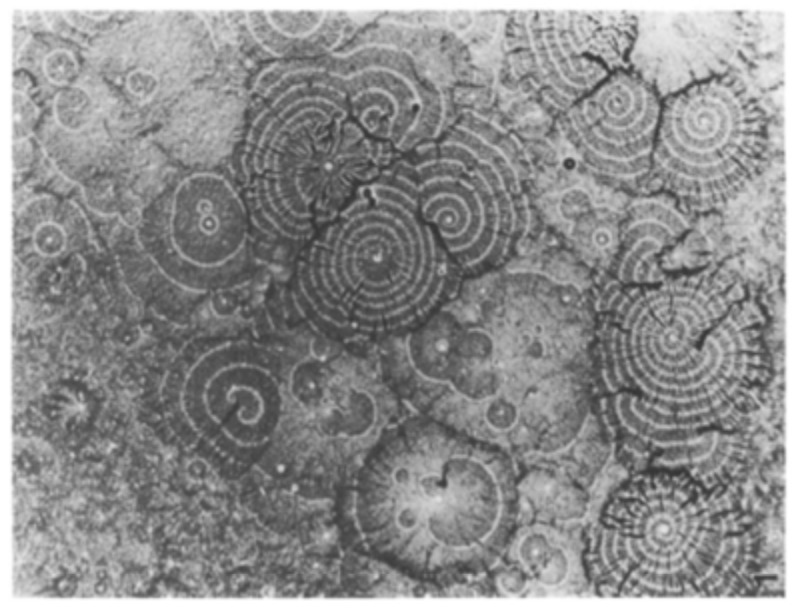
\includegraphics{CG-14-355_F2.jpg}

}

\caption{\label{fig-dicty_spiral}Spiral wave patterns underly
Dictystelium aggregation. Image from Durston (2013).}

\end{figure}

\begin{itemize}
\tightlist
\item
  can we simulate/model the mechanisms regulate that give rise to
  cellular aggregation?
\item
  how do features of patterns that form (e.g.~pattern wavelength, speepd
  of aggregation) depend on individual cell properties?
\end{itemize}

\hypertarget{model-derivation}{%
\section{Model derivation}\label{model-derivation}}

We consider a model for Dicty aggregation through the secretion of and
chemotactic response to cAMP. We denote by \(n({\mathbf{x}}, t)\) the
density of amoebae and \(a({\mathbf{x}}, t)\) the concentration of cAMP.
The general conservation equation for the amoebae can be written:

\[
\frac{\partial n}{\partial  t} + \nabla \cdot {\mathbf{J}} = f(n,a),
\] where \(f(n,a)\) models any reaction terms for the amoebae
e.g.~proliferation, and the flux is given by \[
{\mathbf{J}} = {\mathbf{J}}_{diffusion} + {\mathbf{J}}_{chemotaxis}.
\]

Assuming Fickian diffusion and the general chemotactic flux stated
earlier (Section~\ref{sec-conservation}), the general
\emph{reaction-diffusion-chemotaxis} model for the amoebae responding to
cAMP is given by:

\[
\begin{aligned}
\frac{\partial n}{\partial  t} &=  \underbrace{D_n \nabla^2 n}_{diffusion} - \underbrace{\nabla \cdot \left( \chi(a) n \nabla a \right)}_{chemotaxis} + f(n,a),   \\
\frac{\partial a}{\partial  t} & =   D_a \nabla^2 a + g(n,a), 
\end{aligned}
\]

where we have assumed Fickian diffusion for the cAMP and \(g(a,n)\)
represents the kinetics i.e.~source/sink terms, of cAMP.

One simple model has the following assumptiond:

\[f(n,a) = 0, \;\;\; g(n,a) = \mu n - \delta a, \;\;\; \chi (a) = \chi_0\]

i.e.~

\begin{itemize}
\item
  there are no kinetics for the amoebae - they simply move randomly via
  diffusion and undergo chemotaxis in response to cAMP;
\item
  proliferation is neglected; - this is a reasonable assumption given
  the timescales involved, since they amoebae move on a faster timescale
  than they proliferate;
\item
  the amoebae are assumed to produce cAMP in proportion to their
  density, which means the more amoebae there are, the more cAMP (a
  reasonable first approximation);
\item
  the chemotactic function is taken to be a constant, again a reasonable
  first approximation;
\item
  \(D_a > D_n\) since chemicals diffuse faster than cells move randomly.
\end{itemize}

Under such assumptions we obtain the model equation

\[
\begin{aligned}
\frac{\partial n}{\partial  t} & =  D_n \nabla^2 n - \chi_0 \nabla \cdot \left( n \nabla a \right), \\
\frac{\partial a}{\partial  t} & =   D_a \nabla^2 a +  \mu n - \delta a,
\end{aligned}
\]

which becomes, upon considering a 1-dimensional domain \([0,L]\),

\begin{equation}\protect\hypertarget{eq-chemotaxis1d}{}{
\begin{aligned}
\frac{\partial n}{\partial  t} &=  D_n \frac{\partial ^2 n}{\partial x^2} - \chi_0 \frac{\partial}{\partial x} \left( n \frac{\partial a}{\partial x} \right), \\
  & & \hspace{4.5cm} ( \dagger ) \\
\frac{\partial a}{\partial  t} &=  D_a \frac{\partial ^2 a}{\partial x^2}  +  \mu n - \delta a,
\end{aligned}
}\label{eq-chemotaxis1d}\end{equation}

with zero flux boundary conditions:

\[
\begin{aligned}
D_a \frac{\partial a}{\partial  x} & =  0, \;\;\; x = 0,L, \\
D_n \frac{\partial n}{\partial  x} - \chi_0 n \frac{\partial a}{\partial  x} & =  0, \;\;\; x = 0,L.
\end{aligned}
\]

These reduce to:

\[
\frac{\partial a}{\partial  x} = \frac{\partial n}{\partial  x} = 0, \;\;\; x = 0,L.
\]

\hypertarget{numerical-solutions-4}{%
\section{Numerical solutions}\label{numerical-solutions-4}}

In Figure~\ref{fig-bacterialchemotaxispde} we plot numerical solution of
Equation~\ref{eq-chemotaxis1d} together with no-flux boundary condition.
The initial data are uniformly sampled. Note the emergence of periodic
spatial structure in both variables. These correspond to peaks and
troughs of cell density. The cells produce chemoattractant, \(a\), and
the this induces a chemtactic flux up the gradient in \(a\). Hence more
cells move towards regions where \(a\) is high, more chemoattractant is
produced in this region etc.

\begin{itemize}
\tightlist
\item
  What is the long-time behaviour of these solutions
\item
  For which parameters do we expect to see pattern formation?
\item
  How does spatial pattern depend on the initial data?
\end{itemize}

\begin{Shaded}
\begin{Highlighting}[]
\ImportTok{import}\NormalTok{ numpy }\ImportTok{as}\NormalTok{ np}
\ImportTok{from}\NormalTok{ scipy.integrate }\ImportTok{import}\NormalTok{ odeint}
\ImportTok{import}\NormalTok{ matplotlib.pyplot }\ImportTok{as}\NormalTok{ plt}
\ImportTok{import}\NormalTok{ random}


\NormalTok{T}\OperatorTok{=}\DecValTok{80}
\NormalTok{L}\OperatorTok{=}\DecValTok{150}

\NormalTok{mu}\OperatorTok{=}\FloatTok{1.2}
\NormalTok{delta}\OperatorTok{=}\FloatTok{0.1}
\NormalTok{D\_n}\OperatorTok{=}\FloatTok{2.50}
\NormalTok{D\_a}\OperatorTok{=}\FloatTok{2.5}
\NormalTok{chi\_0}\OperatorTok{=}\FloatTok{1.4}

\NormalTok{N\_x}\OperatorTok{=}\DecValTok{200}
\NormalTok{N\_t}\OperatorTok{=}\DecValTok{100}

\NormalTok{t}\OperatorTok{=}\NormalTok{np.linspace(}\DecValTok{1}\NormalTok{,T,N\_t)}
\NormalTok{x}\OperatorTok{=}\NormalTok{np.linspace(}\DecValTok{0}\NormalTok{,L,N\_x)}

\NormalTok{u\_0}\OperatorTok{=}\NormalTok{np.ones\_like(x)}\OperatorTok{+}\FloatTok{0.01}\OperatorTok{*}\NormalTok{np.random.uniform(low}\OperatorTok{=}\FloatTok{0.0}\NormalTok{, high}\OperatorTok{=}\FloatTok{0.1}\NormalTok{, size}\OperatorTok{=}\NormalTok{(N\_x,))}
\NormalTok{n\_0}\OperatorTok{=}\NormalTok{np.ones\_like(x)}

\NormalTok{u\_0}\OperatorTok{=}\NormalTok{np.concatenate((u\_0,n\_0))}

\NormalTok{dx}\OperatorTok{=}\NormalTok{L}\OperatorTok{/}\NormalTok{(N\_x}\OperatorTok{{-}}\DecValTok{1}\NormalTok{)}
\NormalTok{dt}\OperatorTok{=}\NormalTok{T}\OperatorTok{/}\NormalTok{(N\_t}\OperatorTok{{-}}\DecValTok{1}\NormalTok{)}

\KeywordTok{def}\NormalTok{ LVPDErhs(sol,t):}

\NormalTok{    N\_x}\OperatorTok{=}\BuiltInTok{int}\NormalTok{(np.ceil(}\BuiltInTok{len}\NormalTok{(sol)}\OperatorTok{/}\DecValTok{2}\NormalTok{))}

\NormalTok{    n}\OperatorTok{=}\NormalTok{sol[}\DecValTok{0}\NormalTok{:N\_x]}
\NormalTok{    a}\OperatorTok{=}\NormalTok{sol[N\_x:}\DecValTok{2}\OperatorTok{*}\NormalTok{N\_x]}



\NormalTok{    f\_n}\OperatorTok{=}\NormalTok{np.zeros\_like(n)}
\NormalTok{    f\_a}\OperatorTok{=}\NormalTok{np.zeros\_like(n)}

    \ControlFlowTok{for}\NormalTok{ i }\KeywordTok{in} \BuiltInTok{range}\NormalTok{(}\DecValTok{1}\NormalTok{,N\_x}\OperatorTok{{-}}\DecValTok{2}\NormalTok{):}
\NormalTok{      f\_n[i]}\OperatorTok{=}\NormalTok{D\_n}\OperatorTok{/}\NormalTok{dx}\OperatorTok{**}\DecValTok{2}\OperatorTok{*}\NormalTok{(n[i}\OperatorTok{{-}}\DecValTok{1}\NormalTok{]}\OperatorTok{{-}}\DecValTok{2}\OperatorTok{*}\NormalTok{n[i]}\OperatorTok{+}\NormalTok{n[i}\OperatorTok{+}\DecValTok{1}\NormalTok{]) }\OperatorTok{{-}}\NormalTok{ chi\_0}\OperatorTok{*}\NormalTok{n[i]}\OperatorTok{*}\DecValTok{1}\OperatorTok{/}\NormalTok{dx}\OperatorTok{**}\DecValTok{2}\OperatorTok{*}\NormalTok{(a[i}\OperatorTok{{-}}\DecValTok{1}\NormalTok{]}\OperatorTok{{-}}\DecValTok{2}\OperatorTok{*}\NormalTok{a[i]}\OperatorTok{+}\NormalTok{a[i}\OperatorTok{+}\DecValTok{1}\NormalTok{])}\OperatorTok{{-}}\NormalTok{chi\_0}\OperatorTok{/}\NormalTok{(}\DecValTok{2}\OperatorTok{*}\NormalTok{dx)}\OperatorTok{**}\DecValTok{2}\OperatorTok{*}\NormalTok{(a[i}\OperatorTok{+}\DecValTok{1}\NormalTok{]}\OperatorTok{{-}}\NormalTok{a[i}\OperatorTok{{-}}\DecValTok{1}\NormalTok{])}\OperatorTok{*}\NormalTok{(n[i}\OperatorTok{+}\DecValTok{1}\NormalTok{]}\OperatorTok{{-}}\NormalTok{n[i}\OperatorTok{{-}}\DecValTok{1}\NormalTok{])}

\NormalTok{    i}\OperatorTok{=}\DecValTok{0}
\NormalTok{    f\_n[i]}\OperatorTok{=}\NormalTok{D\_n}\OperatorTok{/}\NormalTok{dx}\OperatorTok{**}\DecValTok{2}\OperatorTok{*}\NormalTok{(}\OperatorTok{{-}}\NormalTok{n[i]}\OperatorTok{+}\NormalTok{n[i}\OperatorTok{+}\DecValTok{1}\NormalTok{]) }\OperatorTok{{-}}\NormalTok{ chi\_0}\OperatorTok{*}\NormalTok{n[i]}\OperatorTok{*}\DecValTok{1}\OperatorTok{/}\NormalTok{(}\DecValTok{2}\OperatorTok{*}\NormalTok{dx)}\OperatorTok{**}\DecValTok{2}\OperatorTok{*}\NormalTok{(}\OperatorTok{{-}}\NormalTok{a[i]}\OperatorTok{+}\NormalTok{a[i}\OperatorTok{+}\DecValTok{1}\NormalTok{])}\OperatorTok{{-}}\NormalTok{chi\_0}\OperatorTok{/}\NormalTok{(}\DecValTok{2}\OperatorTok{*}\NormalTok{dx)}\OperatorTok{**}\DecValTok{2}\OperatorTok{*}\NormalTok{(a[i}\OperatorTok{+}\DecValTok{1}\NormalTok{]}\OperatorTok{{-}}\NormalTok{a[i])}\OperatorTok{*}\NormalTok{(n[i}\OperatorTok{+}\DecValTok{1}\NormalTok{]}\OperatorTok{{-}}\NormalTok{n[i])}

\NormalTok{    i}\OperatorTok{=}\NormalTok{N\_x}\OperatorTok{{-}}\DecValTok{1}
\NormalTok{    f\_n[i]}\OperatorTok{=}\NormalTok{D\_n}\OperatorTok{/}\NormalTok{dx}\OperatorTok{**}\DecValTok{2}\OperatorTok{*}\NormalTok{(n[i}\OperatorTok{{-}}\DecValTok{1}\NormalTok{]}\OperatorTok{{-}}\NormalTok{n[i])}\OperatorTok{{-}}\NormalTok{ chi\_0}\OperatorTok{*}\NormalTok{n[i]}\OperatorTok{*}\DecValTok{1}\OperatorTok{/}\NormalTok{(}\DecValTok{2}\OperatorTok{*}\NormalTok{dx)}\OperatorTok{**}\DecValTok{2}\OperatorTok{*}\NormalTok{(a[i}\OperatorTok{{-}}\DecValTok{1}\NormalTok{]}\OperatorTok{{-}}\NormalTok{a[i])}\OperatorTok{{-}}\NormalTok{chi\_0}\OperatorTok{/}\NormalTok{(}\DecValTok{2}\OperatorTok{*}\NormalTok{dx)}\OperatorTok{**}\DecValTok{2}\OperatorTok{*}\NormalTok{(a[i]}\OperatorTok{{-}}\NormalTok{a[i}\OperatorTok{{-}}\DecValTok{1}\NormalTok{])}\OperatorTok{*}\NormalTok{(n[i]}\OperatorTok{{-}}\NormalTok{n[i}\OperatorTok{{-}}\DecValTok{1}\NormalTok{])}


    \ControlFlowTok{for}\NormalTok{ i }\KeywordTok{in} \BuiltInTok{range}\NormalTok{(}\DecValTok{1}\NormalTok{,N\_x}\OperatorTok{{-}}\DecValTok{2}\NormalTok{):}
\NormalTok{      f\_a[i]}\OperatorTok{=}\NormalTok{D\_a}\OperatorTok{/}\NormalTok{dx}\OperatorTok{**}\DecValTok{2}\OperatorTok{*}\NormalTok{(a[i}\OperatorTok{{-}}\DecValTok{1}\NormalTok{]}\OperatorTok{{-}}\DecValTok{2}\OperatorTok{*}\NormalTok{a[i]}\OperatorTok{+}\NormalTok{a[i}\OperatorTok{+}\DecValTok{1}\NormalTok{]) }
\NormalTok{    i}\OperatorTok{=}\DecValTok{0}
\NormalTok{    f\_a[i]}\OperatorTok{=}\NormalTok{D\_a}\OperatorTok{/}\NormalTok{dx}\OperatorTok{**}\DecValTok{2}\OperatorTok{*}\NormalTok{(}\OperatorTok{{-}}\NormalTok{a[i]}\OperatorTok{+}\NormalTok{a[i}\OperatorTok{+}\DecValTok{1}\NormalTok{]) }
\NormalTok{    i}\OperatorTok{=}\NormalTok{N\_x}\OperatorTok{{-}}\DecValTok{1}
\NormalTok{    f\_a[i]}\OperatorTok{=}\NormalTok{D\_a}\OperatorTok{/}\NormalTok{dx}\OperatorTok{**}\DecValTok{2}\OperatorTok{*}\NormalTok{(a[i}\OperatorTok{{-}}\DecValTok{1}\NormalTok{]}\OperatorTok{{-}}\NormalTok{a[i])}

\NormalTok{    reaction\_n}\OperatorTok{=}\DecValTok{0}
\NormalTok{    reaction\_a}\OperatorTok{=}\NormalTok{mu}\OperatorTok{*}\NormalTok{n}\OperatorTok{{-}}\NormalTok{delta}\OperatorTok{*}\NormalTok{a}

\NormalTok{    f\_n}\OperatorTok{=}\NormalTok{f\_n}\OperatorTok{+}\NormalTok{reaction\_n}
\NormalTok{    f\_a}\OperatorTok{=}\NormalTok{f\_a}\OperatorTok{+}\NormalTok{reaction\_a}

\NormalTok{    f}\OperatorTok{=}\NormalTok{ np.concatenate((f\_n, f\_a)) }
    \ControlFlowTok{return}\NormalTok{ f  }

\NormalTok{sol}\OperatorTok{=}\NormalTok{odeint(LVPDErhs,u\_0,t)}

\NormalTok{n}\OperatorTok{=}\NormalTok{sol[:,}\DecValTok{0}\NormalTok{:N\_x]}
\NormalTok{a}\OperatorTok{=}\NormalTok{sol[:,}\DecValTok{0}\NormalTok{:N\_x]}

\NormalTok{fig, ax }\OperatorTok{=}\NormalTok{ plt.subplots(}\DecValTok{2}\NormalTok{,}\DecValTok{1}\NormalTok{)}

\NormalTok{ax[}\DecValTok{0}\NormalTok{].plot(x,n[}\DecValTok{0}\NormalTok{,:],}\StringTok{\textquotesingle{}r\textquotesingle{}}\NormalTok{)}
\NormalTok{ax[}\DecValTok{0}\NormalTok{].plot(x,n[}\DecValTok{16}\NormalTok{,:],}\StringTok{\textquotesingle{}b\textquotesingle{}}\NormalTok{)}
\NormalTok{ax[}\DecValTok{0}\NormalTok{].plot(x,n[}\DecValTok{32}\NormalTok{,:],}\StringTok{\textquotesingle{}m\textquotesingle{}}\NormalTok{)}
\NormalTok{ax[}\DecValTok{0}\NormalTok{].plot(x,n[}\DecValTok{48}\NormalTok{,:],}\StringTok{\textquotesingle{}k\textquotesingle{}}\NormalTok{)}
\NormalTok{ax[}\DecValTok{0}\NormalTok{].set\_xlabel(}\StringTok{\textquotesingle{}$x$\textquotesingle{}}\NormalTok{)}
\NormalTok{ax[}\DecValTok{0}\NormalTok{].set\_ylabel(}\StringTok{\textquotesingle{}$n$\textquotesingle{}}\NormalTok{)}

\NormalTok{ax[}\DecValTok{1}\NormalTok{].plot(x, a[}\DecValTok{0}\NormalTok{,:],}\StringTok{\textquotesingle{}r{-}{-}\textquotesingle{}}\NormalTok{)}
\NormalTok{ax[}\DecValTok{1}\NormalTok{].plot(x, a[}\DecValTok{16}\NormalTok{,:],}\StringTok{\textquotesingle{}b{-}{-}\textquotesingle{}}\NormalTok{)}
\NormalTok{ax[}\DecValTok{1}\NormalTok{].plot(x, a[}\DecValTok{32}\NormalTok{,:],}\StringTok{\textquotesingle{}m{-}{-}\textquotesingle{}}\NormalTok{)}
\NormalTok{ax[}\DecValTok{1}\NormalTok{].plot(x, a[}\DecValTok{48}\NormalTok{,:],}\StringTok{\textquotesingle{}k{-}{-}\textquotesingle{}}\NormalTok{)}
\NormalTok{ax[}\DecValTok{1}\NormalTok{].set\_xlabel(}\StringTok{\textquotesingle{}$x$\textquotesingle{}}\NormalTok{)}
\NormalTok{ax[}\DecValTok{1}\NormalTok{].set\_ylabel(}\StringTok{\textquotesingle{}$a$\textquotesingle{}}\NormalTok{)}

\NormalTok{plt.legend([}\StringTok{\textquotesingle{}t\textquotesingle{}}\OperatorTok{+} \BuiltInTok{str}\NormalTok{(t[}\DecValTok{0}\NormalTok{]),}\StringTok{\textquotesingle{}t=\textquotesingle{}}\OperatorTok{+} \BuiltInTok{str}\NormalTok{(t[}\DecValTok{4}\NormalTok{]),}\StringTok{\textquotesingle{}t=\textquotesingle{}}\OperatorTok{+} \BuiltInTok{str}\NormalTok{(t[}\DecValTok{8}\NormalTok{]),}\StringTok{\textquotesingle{}t=\textquotesingle{}}\OperatorTok{+} \BuiltInTok{str}\NormalTok{(t[}\DecValTok{12}\NormalTok{])])}
\NormalTok{plt.xlabel(}\StringTok{\textquotesingle{}$x$\textquotesingle{}}\NormalTok{)}
\NormalTok{plt.grid()}
\NormalTok{plt.show()}
\end{Highlighting}
\end{Shaded}

\begin{figure}[H]

{\centering 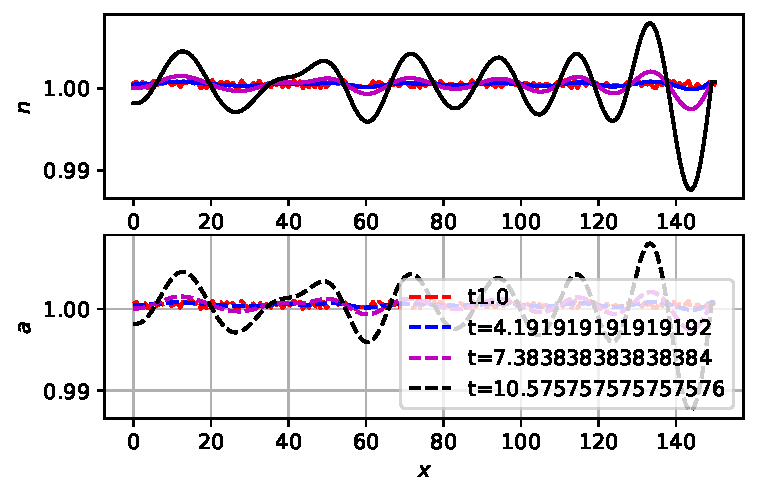
\includegraphics{BacterialChemotaxis_files/figure-pdf/fig-bacterialchemotaxispde-output-1.pdf}

}

\caption{\label{fig-bacterialchemotaxispde}Numerical solution of
bacterial chemtaxis model}

\end{figure}

\hypertarget{spatially-homogeneous-steady-states-1}{%
\section{Spatially Homogeneous Steady
States}\label{spatially-homogeneous-steady-states-1}}

Define the total number of cells, \(N\), \[
N= \int_0^L n(x,t)dx
\] Upon differentiation with respect to time \[
\begin{aligned}
\frac{dN}{dt} &=\int_0^L \frac{\partial n(x,t)}{\partial t}dx
&=\int_0^L  D_n \frac{\partial ^2 n}{\partial x^2} - \chi_0 \frac{\partial}{\partial x} \left( n \frac{\partial a}{\partial x} \right) dx.
\end{aligned}
\] Upon integration of the right-hand side w.r.t. \(x\), subsequent
application of the no-flux boundary condition implies \[
\frac{dN}{dt}=0.
\] Hence the total number of cells in the domain is fixed by the initial
data. For a spatially homogeneoud solutions, th4 cells must be uniformly
distributed in space, i.e. \[
n^*=N/L
\]

Additionaly, the spatially homogeneous steady state solution
\((n^* , a^* )\) satisfies:

\[
a^*=\frac{\mu}{\delta} n^*.
\]

We now undertake a linear stability analysis to determine whether this
is stable or unstable. If the above spatially homogeneous steady state
is unstable, this will indicate that aggregation patterns may arise in
the system.

\hypertarget{stability-analysis}{%
\section{Stability Analysis}\label{stability-analysis}}

In a similar manner to previous stability analyses, we consider small
perturbations around the spatially homogeneous steady state
\((n^* , a^* )\), i.e.

\[
n(x,t) = n^* + \tilde{n}(x,t), \;\;\; a(x,t) = a^* + \tilde{a}(x,t)
\]

where \(\tilde{n}(x,t)\) and \(\tilde{a}(x,t)\) are ``small'' so that
higher order terms can be neglected.

\textbf{NOTE} Unlike previous stability analysis, these perturbations
are both \emph{time} and \emph{space} dependent.

Substituting the above perturbations into equations \(( \dagger )\), we
neglect higher order terms and retain only linear terms. This is largely
straightforward, but we provide some detail for the linearization of the
chemotactic term i.e.~

\[
\frac{\partial}{\partial x} \left[ ( n^* + \tilde{n}) \frac{\partial}{\partial x} \left( a^* + \tilde{a} \right) \right] = \frac{\partial}{\partial x} \left[ ( n^* + \tilde{n}) \frac{\partial \tilde{a}}{\partial x}  \right] \approx n^* \frac{\partial ^2 \tilde{a}}{\partial x^2}.
\]

The fully linearized system is then given by:
\begin{equation}\protect\hypertarget{eq-chemotax_linear}{}{
\begin{aligned}
\frac{\partial \tilde{n}}{\partial  t} & =  D_n \frac{\partial ^2 \tilde{n}}{\partial x^2} - \chi_0 n^* \frac{\partial ^2 \tilde{a}}{\partial x^2} \\
\frac{\partial \tilde{a}}{\partial  t} & =   D_a \frac{\partial ^2 \tilde{a}}{\partial x^2}  +  \mu \tilde{n} - \delta \tilde{a}.
\end{aligned}
}\label{eq-chemotax_linear}\end{equation}

Although the above equations are linear, an explicit solution is
non-trivial and we are required to make a further ``separation of
variables'' \emph{ansatz}. We seek solutions of the form \[
\tilde{n}(t,x) = u(t) \phi_1(x)
\] and \[
\tilde a (t,x) = v(t) \phi_2(x)
\]

Upon substitution \[
\begin{aligned}
&\frac{\partial u}{\partial  t}  \phi_1  =   D_n  u\frac{\partial ^2 \phi_1}{\partial x^2} - \chi_0 n^*  v\frac{\partial ^2 \phi_1}{\partial x^2} \\
& \frac{\partial v}{\partial  t}  \phi_2=     D_a v \frac{\partial ^2  \phi_2}{\partial x^2}  +  \mu u \,  \phi_1 - \delta v\,  \phi_2, \\
\end{aligned}
\] with boundary conditions \[
\begin{aligned}
& u \frac{\partial \phi_1}{\partial x} = 0, \quad   v \frac{\partial \phi_2}{\partial x} = 0 \quad \text{ for } \; x = 0, \; x=L.
\end{aligned}
\]

We assume that\\
\[
\phi_1 = \phi_2 = \phi,
\] where \(\phi\) is the solution of the elliptic problem \[
\begin{aligned}
\frac{d^2 \phi}{dx^2} &= - k^2 \phi && \text{ in } \; (0,L), \\
\frac{d \phi}{dx} &= 0  && \text{ for } \; x=0, \; x=L. 
\end{aligned}
\] We can compute that solution of the equation for \(\phi\) are of the
form \[
\phi(x) = A \cos(kx) + B\sin(kx).
\] Since \(\phi\) satisfied zero Neumann boundary conditions we have
that \[
\phi(x) = A \cos(kx),
\] where \(A\) is an arbitrary constanr, and \[
k = \dfrac {m \pi} L, \quad m \in \mathbb N.
\]

Then we have \[
\begin{aligned}
&\frac{\partial u}{\partial  t}  \phi  =   - k^2 D_n  u \phi +  \chi_0 n^* k^2\,  v \, \phi,  \\
& \frac{\partial v}{\partial  t} \phi =   - k^2 D_a  \, v \phi  +  \mu u \,  \phi - \delta v\,  \phi, 
\end{aligned}
\] and since \(\phi\) is not identically zero on \((0,L)\) we obtain a
system of linear ODEs for \((u(t),v(t))\) \[
\begin{aligned}
&\frac{\partial u}{\partial  t}    =   - k^2 D_n  u  +  \chi_0 n^* k^2\,  v,  \\
& \frac{\partial v}{\partial  t} =   - k^2 D_a  \, v  +  \mu u  - \delta v. 
\end{aligned}
\]

We know that solutions of linear ODEs have the form \[
u(t) = C_1 e^{\lambda t} \quad \textrm{and} \quad v(t) = C_2 e^{\lambda t}
\] for some constant \(C_1\), \(C_2\) and \(\lambda\) are eigenvalues of
the corresponding matrix.

Thus we obtain \[
\begin{aligned}
\lambda C_1 & =  - D_n k^2 C_1  + \chi_0 n^* k^2 C_2,  \\
\lambda C_2 & = - D_a k^2 C_2 +  \mu C_1 - \delta C_2,
\end{aligned}
\] which can be written

\[
\left(
\begin{array}{cc}
- D_n k^2 - \lambda &  \chi_0 n^* k^2 \\
\mu & - D_a k^2 -\delta -\lambda 
\end{array}
\right) 
\left(
\begin{array}{c}
C_1 \\
C_2
\end{array}
\right) = \mathbf{0} .
\]

\textbf{Remark} Notice that we obtained that \(\tilde n\) and
\(\tilde a\) are of the form
\[\tilde{n}(x,t) = C_1 e^{\lambda t} e^{ikx}, \;\;\; \tilde{a}(x,t) = C_2 e^{\lambda t} e^{ikx}.\]

For a non-trivial solution (for non-trivial perturbations \(\tilde n\),
\(\tilde a\)), i.e.~\(C_1 \neq 0\) and \(C_2 \neq 0\), the determinant
of the above matrix must be zero, and this leads to the following
quadratic equation to be solved for \(\lambda\):

\[
\lambda^2 + \left( D_n k^2 + D_a k^2 + \delta \right) \lambda + D_n k^2 \left( D_a k^2 + \delta \right) - \mu \chi_0 n^* k^2 = 0.
\]

This is of the form \[
\lambda^2 + \alpha \lambda + \beta = 0,
\]

and so has roots: \[
\lambda = \frac{-\alpha \pm \sqrt{\alpha^2 - 4 \beta}}{2}.\]

\textbf{NOTE} This has two \emph{real} roots, since \[
\alpha^2 - 4 \beta > 0
\] (see Exercise/Tutorial).

For stability, we require both roots to be negative. Since both roots
are real, this leads to:

\[
\lambda < 0  \Leftrightarrow \alpha > 0 \;\;\; \text{and} \;\;\; \beta >0.
\]

Now \[\alpha = D_n k^2 + D_a k^2 + \delta > 0,
\] and so for stability, we require \(\beta > 0\) i.e.~

\[
\begin{aligned}
& & D_n k^2 \left( D_a k^2 + \delta \right) - \mu \chi_0 n^* k^2 > 0 \\
& & \Rightarrow \mu \chi_0 n^* <  D_n  \left( D_a k^2 + \delta \right)
\end{aligned}
\] Hence, we will have instability when this condition is not satisfied
i.e.~ \[
\mu \chi_0 n^* >  D_n  \left( D_a k^2 + \delta \right).
\]

The precise value of \(k^2\) can be determined from the zero-flux
boundary conditions i.e. \[ 
k  =  \frac{m \pi}{L}, \;\;\; m = 1,2, \dots 
\] if we look for non-constant \(\phi\).

Hence, we will have instability whenever \[
\mu \chi_0 n^* >  D_n  \left( D_a \frac{m^2 \pi^2}{L^2} + \delta \right), \;\;\; m = 1,2, \dots
\]

It can be shown (see Exercise/Tutorial), that \(\lambda (k^2)\) ( or
\(\lambda (m^2)\)) is monotonic decreasing and hence the fastest growing
mode is \(m=1\) i.e.~we have an instability as long as \[
\mu \chi_0 n^* >  D_n  \left( \frac{D_a \pi^2}{L^2} + \delta \right).
\]

In general, from the above inequality, we can say that there is a
likelihood of instability (amoebae aggregation) if:

\begin{itemize}
\tightlist
\item
  \(D_a\), \(D_n\) and \(\delta\) are all ``small'\,'
\item
  L is ``large'\,'
\item
  \(\chi_0 , \mu , n^*\) are ``large'\,'
\end{itemize}

Considering all other parameters to be fixed, in theory the above result
states that it is possible to find a large enough value for the
chemotactic coefficient \(\chi_0\) to satisfy the instability condition
i.e.~chemotaxis induces instability and leads to aggregation of the
amoebae.

\hypertarget{exercise-1}{%
\section{Exercise}\label{exercise-1}}

From the results we have obtained we deduce that:

\begin{itemize}
\tightlist
\item
  chemotaxis has a destabilizing effect
\item
  diffusion has a stabilizing effect on spatially homogeneous solutions
\end{itemize}

If this is true then one might expect the numerical results presented in
Figure~\ref{fig-bacterialchemotaxispde} to have spatially homogeneous
solutions if the diffusion coefficient is made sufficiently large. * Can
you test this by running the code for larger values of the parameter
\(D\)? * Alternatively, what happens if you make the chemotactic
coefficient \(\chi_0\) smaller? * what kind of aggregation patterns do
you see if the system is solved in two spatial dimensions?

However, there is one type of system where diffusion also has a
destabilizing effect\ldots{}

\hypertarget{diffusion-driven-instability}{%
\chapter{Diffusion driven
instability}\label{diffusion-driven-instability}}

\hypertarget{spatial-pattern-formation-via-reaction-diffusion-mechanisms}{%
\section{Spatial Pattern Formation via Reaction-Diffusion
Mechanisms}\label{spatial-pattern-formation-via-reaction-diffusion-mechanisms}}

** Insert human embryogenesis image **

\hypertarget{pattern-in-developmental-biology}{%
\subsection{Pattern in Developmental
Biology}\label{pattern-in-developmental-biology}}

Embryology or developmental biology is that part of biology which is
concerned with the formation, growth and development of the embryo from
fertilization until birth. From the very moment of conception the embryo
undergoes a process of dynamic change, brought about largely by cells
responding to various chemical signalling cues e.g.~migration,
differentiation, proliferation. Figure \ref{embryogenesis} shows some of
the major changes in embryonic development which occur up to a few weeks
after fertilization. Many of the processes occurring at this early stage
are vital for the successful subsequent development of the embryo and
also lay down basic structures
(e.g.~\href{https://en.wikipedia.org/wiki/Somite}{somites}) that form
the foundation of major body structures later on (e.g.~the vertebrae of
the spine) cf.~Professor Lewis Wolpert: `\emph{It is not birth,
marriage, or death, but gastrulation which is truly the most important
time in your life.}'

There are two main theories which describe how pattern arises during
embryogenesis - one is the \textbf{Turing pre-pattern theory}, the other
is the \textbf{mechano-chemical} theory. In the Turing pre-pattern
theory, chemicals, or
\href{https://en.wikipedia.org/wiki/Morphogen}{morphogens}, react
together and, if certain conditions concerning their reaction kinetics
and diffusion rates are satisfied (to be derived in the next section),
then a \#\# pre-pattern\#\# of varying chemical concentrations is set up
in the spatial domain. This means that throughout the spatial domain,
the concentration levels of the chemicals will vary i.e.~there will be a
\#\#heterogeneous\#\# distribution of chemical concentrations which is
known as a pre-pattern. Any cells in the domain which subsequently
encounter these varying levels of morphogens will then respond by, for
example, proliferating differentially throughout the domain. In this
way, the domain will then contain a \{spatially heterogeneous\}
distribution of cell densities (i.e.~a cellular pattern) which have
responded to the morphogen pre-pattern. This pre-pattern theory was
first proposed by Alan Turing (of Enigma Code fame) in his seminal 1952
paper, \emph{The chemical basis of morphogenesis} Turing (1990). This
was developed in more detailed manner by Alfred Gierer and Hans
Meinhardt in another ground-breaking paper in 1972, \emph{A theory of
biological pattern formation} {``A Theory of Biological Pattern
Formation''} (1972), where they introduced the concept of activating
chemicals and inhibiting chemicals. J.D. Murray then applied the theory
as an explanation for the generation of patterns observed on animal
coats J. Murray (1981).

In the mechano-chemical theory, cells interact with their surroundings
and by exerting forces perturb their local environment. The combination
of cell migration/proliferation and cell-generated forces is sufficient
in certain circumstances to create a spatially heterogeneous
distribution of cell densities i.e.~the pattern is generated
\textbf{simultaneously} with the cell migration/proliferation. This
alternative pattern formation theory was proposed by Murray and Oster
James D. Murray and Oster (1984) and is particularly appropriate for
patterns generated in early embryogenesis by \textbf{mesenchymal cells}
such as fibroblasts.

\hypertarget{reaction-diffusion-turing-pre-pattern-mechanisms}{%
\section{Reaction-diffusion (Turing) Pre-pattern
Mechanisms}\label{reaction-diffusion-turing-pre-pattern-mechanisms}}

We now consider our general (dimensional) reaction-diffusion model for
two chemicals or morphogens with concentrations \(A({\mathbf{x}}, t)\)
and \(B({\mathbf{x}}, t)\) which react together and diffuse in some
spatial domain:

\[
\begin{aligned}
\frac{\partial A}{\partial  t} & =  F(A,B)  + D_A \nabla^2 A, \\
\frac{\partial B}{\partial  t} & =  G(A,B)  + D_B \nabla^2 B,
\end{aligned}
\]

where \(F(A,B)\) and \(G(A,B)\) describe the reaction kinetics between
the two morphogens and \(D_A, D_B > 0\) are the diffusion coefficients.
Turing's theory (Turing, 1952) \emph{The chemical basis of
morphogenesis} proposed that it was the diffusion of the substances
\(A, B\) which led to the evolution of a spatially heterogeneous
solution to arise i.e.~a spatial pattern. This has given rise to the
phrase \emph{diffusion-driven instability}. This was a rather
revolutionary and counter-intuitive proposal, since, as we have seen,
diffusion normally has the opposite tendency i.e.~to smooth or average
out spatial heterogeneities, and to give rise to spatially homogeneous
solutions.

Various forms can be considered for the kinetic functions \(F\) and
\(G\). However, we will focus mainly on three specific classes as
follows:

\hypertarget{schnackenberg-kinetics}{%
\subsection{Schnackenberg kinetics}\label{schnackenberg-kinetics}}

\[
F(A,B) = k_1 - k_2 A + k_3 A^2 B, \;\;\;\; G(A,B) = k_4 - k_3 A^2 B
\]

\(k_1, k_2, k_3, k_4 >0\). The term \(k_3 A^2 B\) is
\textbf{autocatalytic}, since the species \(A\) upregulates its own
production.

\hypertarget{gierer-meinhardt-kinetics}{%
\subsection{Gierer \& Meinhardt
kinetics}\label{gierer-meinhardt-kinetics}}

Gierer \& Meinhardt developed a model that describes activator-inhibitor
kinetics. The total reaction rates are \[
F(A,B) = k_1 - k_2 A + \frac{k_3 A^2}{B}, \;\;\;\; G(A,B) = k_4 A^2 - k_5 B
\] where \(k_1, k_2, k_3, k_4 , k_5 > 0\). The term \(k_3 A^2 / B\) is
\textbf{autocatalytic}.

\hypertarget{thomas-kinetics}{%
\subsection{Thomas kinetics}\label{thomas-kinetics}}

Thomas developed a model of substrate inhibition in which \[
\begin{aligned}
F(A,B) &= k_1 - k_2 A - H(A,B), \\
G(A,B) &= k_4 A^2 - k_4 B -H(A,B), \\ 
H(A,B) &= \frac{k_5 AB}{k_6 + k_7 + k_8 A^2}.
\end{aligned}
\] with \(k_i > 0\). In the original paper of Thomas (1975), \(A\)
represents the concentration of oxygen (substrate) and \(B\) the
concentration of uricase (enzyme). Substrate inhibition is evident in
the term \(k_8 A^2\).

\hypertarget{non-dimensionalization}{%
\section{Non-dimensionalization}\label{non-dimensionalization}}

Before proceeding with our analysis, it is prudent to non-dimensionalize
each of the above systems.

\hypertarget{schnakenberg}{%
\subsection{Schnakenberg}\label{schnakenberg}}

We illustrate this process for the Schnakenberg kinetics. Using the
scaling

\[
u = A \left( \frac{k_3}{k_2} \right)^{1/2}, \quad v = B \left( \frac{k_3}{k_2} \right)^{1/2}, \quad t^* = \frac{D_A t}{L^2},\quad x^* = \frac{x}{L},
\]

where \(L\) is a typical length scale, the dimensionless
reaction-diffusion system with Schnakenberg kinetics becomes (upon
dropping the \(*\)):

\begin{equation}\protect\hypertarget{eq-schnackenbergeqns}{}{
\begin{aligned}
\frac{\partial u}{\partial  t} & = \gamma ( a - u + u^2 v ) + \nabla^2 u = \gamma f(u,v)  + \nabla^2 u, \\
\frac{\partial v}{\partial  t} & = \gamma ( b - u^2 v ) + d \nabla^2 v = \gamma g(u,w)  + d \nabla^2 v, 
\end{aligned}
}\label{eq-schnackenbergeqns}\end{equation}

where \[
d = \frac{D_B}{D_A}, \quad a = \frac{k_1}{k_2} \left( \frac{k_3}{k_2} \right)^{1/2}, \quad b = \frac{k_4}{k_2} \left( \frac{k_3}{k_2} \right)^{1/2}, \quad \gamma = \frac{L^2 k_2}{D_A}.
\]

\hypertarget{gierer-meinhardt}{%
\subsection{Gierer-Meinhardt}\label{gierer-meinhardt}}

The Gierer-Meinhardt kinetics can be non-dimensionalized as follows:

\[
\begin{aligned}
f(u, v) & =  a - b u + \frac{u^2}{v}, 
g(u,v) &= u^2 - v, \\
\end{aligned}
\] where \(a , b\) are positive parameters (Exercise/Tutorial).

\hypertarget{thomas}{%
\subsection{Thomas}\label{thomas}}

The Thomas kinetics can be non-dimensionalized as follows:

\[
\begin{aligned}
f(u,v) & =  a - u - h(u,v), \\
g(u,v) &= \alpha (b - v) - h(u,v), \\
h(u,v) & =  \frac{\rho u v}{1 + u + K u^2},
\end{aligned}
\] where \(a , b, \alpha, \rho , K\) are positive parameters
(Exercise/Tutorial).

\hypertarget{general}{%
\subsection{General}\label{general}}

Any reaction-diffusion system can be non-dimensionalized and scaled
following the above procedure to take the following general form:

\[
\begin{aligned}
\frac{\partial u}{\partial  t} & = \gamma f(u,v)  + \nabla^2 u, \\
\frac{\partial v}{\partial  t} & = \gamma g(u,w)  + d \nabla^2 v, 
\end{aligned}
\]

where the parameter \(d\) is the ratio of the diffusion coefficients
from the dimensional system and the parameter \(\gamma\) can be
interpreted in any one of the following ways:

\begin{itemize}
\tightlist
\item
  \(\gamma^{1/2}\) is proportional to the \textbf{linear size} of the
  spatial domain in one-dimension. In two-dimensions, \(\gamma\) is
  proportional to the area.
\item
  \(\gamma\) represents the relative strength of the reaction terms --
  an increase in \(\gamma\) may represent an increase in the activity of
  some rate-limiting step in the reaction sequence.
\item
  An increase in \(\gamma\) is equivalent to a decrease in the diffusion
  coefficient, \(d\).
\end{itemize}

Note that in the case where the parameter \(d > 1\), this means that the
original diffusion coefficients are not equal. Specifically, in the case
of the Gierer-Meinhardt activator-inhibitor system, \(d >1\) implies
that the inhibitor \emph{diffuses more quickly} than the activator
{[}\(d > 1 \Rightarrow D_B > D_A\) {]}. The spatial implications of this
are shown in (\textbf{fig\_ai?}) -- the inhibitor diffuses a greater
distance than the activator, giving rise to what is known as \emph{local
activation, long-range inhibition}.

** Insert activator\_inhibitor here **

\hypertarget{numerical-solution-1}{%
\section{Numerical solution}\label{numerical-solution-1}}

In Figure~\ref{fig-schnack_ddi_pde} we plot numerical solutions of
Equation~\ref{eq-schnackenbergeqns} with no flux boundary conditions.

In this numerical solution the initial condition are the spatially
homogeneous steady state perturbed by uniformly sampled noise. As time
evolves, a spatial pattern emerges. The main idea from a biological
perspeftive is that an unpatterned region of an embryo could undergo
chemical reactions, with the result being a patterned chemcial field.

Some question that might arise:

\begin{itemize}
\tightlist
\item
  How does pattern formation depend on model parameters?
\item
  How does pattern formation depend on domain size?
\item
  How does the pattern wavelength depend on model parameters?
\item
  How does the pattern depend on the initial conditions?
\item
  How can we numerically solve the reaction diffusion PDEs?
\end{itemize}

\begin{Shaded}
\begin{Highlighting}[]
\ImportTok{import}\NormalTok{ numpy }\ImportTok{as}\NormalTok{ np}
\ImportTok{from}\NormalTok{ scipy.integrate }\ImportTok{import}\NormalTok{ odeint}
\ImportTok{from}\NormalTok{ scipy.integrate }\ImportTok{import}\NormalTok{ solve\_ivp}

\ImportTok{import}\NormalTok{ matplotlib.pyplot }\ImportTok{as}\NormalTok{ plt}
\ImportTok{import}\NormalTok{ random}

\NormalTok{T}\OperatorTok{=}\DecValTok{3}
\NormalTok{L}\OperatorTok{=}\DecValTok{1}

\NormalTok{gamma}\OperatorTok{=}\FloatTok{650.0}
\NormalTok{a}\OperatorTok{=}\FloatTok{0.2}
\NormalTok{b}\OperatorTok{=}\FloatTok{1.3}
\NormalTok{d}\OperatorTok{=}\FloatTok{30.0}

\NormalTok{N\_x}\OperatorTok{=}\DecValTok{80}
\NormalTok{N\_t}\OperatorTok{=}\DecValTok{50}

\NormalTok{t}\OperatorTok{=}\NormalTok{np.linspace(}\DecValTok{1}\NormalTok{,T,N\_t)}
\NormalTok{x}\OperatorTok{=}\NormalTok{np.linspace(}\DecValTok{0}\NormalTok{,L,N\_x)}

\NormalTok{u\_0}\OperatorTok{=}\NormalTok{(a}\OperatorTok{+}\NormalTok{b)}\OperatorTok{*}\NormalTok{np.ones\_like(x)}\OperatorTok{+}\FloatTok{0.01}\OperatorTok{*}\NormalTok{np.random.uniform(low}\OperatorTok{={-}}\FloatTok{1.0}\NormalTok{, high}\OperatorTok{=}\FloatTok{1.0}\NormalTok{, size}\OperatorTok{=}\NormalTok{(N\_x,))}
\NormalTok{v\_0}\OperatorTok{=}\NormalTok{b}\OperatorTok{*}\NormalTok{(}\DecValTok{1}\OperatorTok{/}\NormalTok{(a}\OperatorTok{+}\NormalTok{b)}\OperatorTok{**}\DecValTok{2}\NormalTok{)}\OperatorTok{*}\NormalTok{np.ones\_like(x)}\OperatorTok{+}\FloatTok{0.01}\OperatorTok{*}\NormalTok{np.random.uniform(low}\OperatorTok{={-}}\FloatTok{1.0}\NormalTok{, high}\OperatorTok{=}\FloatTok{1.0}\NormalTok{, size}\OperatorTok{=}\NormalTok{(N\_x,))}

\NormalTok{u\_0}\OperatorTok{=}\NormalTok{np.concatenate((u\_0,v\_0))}

\NormalTok{dx}\OperatorTok{=}\NormalTok{L}\OperatorTok{/}\NormalTok{(N\_x}\OperatorTok{{-}}\DecValTok{1}\NormalTok{)}
\NormalTok{dt}\OperatorTok{=}\NormalTok{T}\OperatorTok{/}\NormalTok{(N\_t}\OperatorTok{{-}}\DecValTok{1}\NormalTok{)}

\KeywordTok{def}\NormalTok{ ShcnackPDErhs(sol,t):}

\NormalTok{    N\_x}\OperatorTok{=}\BuiltInTok{int}\NormalTok{(np.ceil(}\BuiltInTok{len}\NormalTok{(sol)}\OperatorTok{/}\DecValTok{2}\NormalTok{))}

\NormalTok{    u}\OperatorTok{=}\NormalTok{sol[}\DecValTok{0}\NormalTok{:N\_x]}
\NormalTok{    v}\OperatorTok{=}\NormalTok{sol[N\_x:]}

\NormalTok{    f\_u}\OperatorTok{=}\NormalTok{np.zeros\_like(u)}
\NormalTok{    f\_v}\OperatorTok{=}\NormalTok{np.zeros\_like(u)}

    \ControlFlowTok{for}\NormalTok{ i }\KeywordTok{in} \BuiltInTok{range}\NormalTok{(}\DecValTok{1}\NormalTok{,N\_x}\OperatorTok{{-}}\DecValTok{2}\NormalTok{):}
\NormalTok{      f\_u[i]}\OperatorTok{=}\DecValTok{1}\OperatorTok{/}\NormalTok{dx}\OperatorTok{**}\DecValTok{2}\OperatorTok{*}\NormalTok{(u[i}\OperatorTok{{-}}\DecValTok{1}\NormalTok{]}\OperatorTok{{-}}\DecValTok{2}\OperatorTok{*}\NormalTok{u[i]}\OperatorTok{+}\NormalTok{u[i}\OperatorTok{+}\DecValTok{1}\NormalTok{]) }

\NormalTok{    i}\OperatorTok{=}\DecValTok{0}
\NormalTok{    f\_u[i]}\OperatorTok{=}\DecValTok{1}\OperatorTok{/}\NormalTok{dx}\OperatorTok{**}\DecValTok{2}\OperatorTok{*}\NormalTok{(}\OperatorTok{{-}}\NormalTok{u[i]}\OperatorTok{+}\NormalTok{u[i}\OperatorTok{+}\DecValTok{1}\NormalTok{])}

\NormalTok{    i}\OperatorTok{=}\NormalTok{N\_x}\OperatorTok{{-}}\DecValTok{1}
\NormalTok{    f\_u[i]}\OperatorTok{=}\DecValTok{1}\OperatorTok{/}\NormalTok{dx}\OperatorTok{**}\DecValTok{2}\OperatorTok{*}\NormalTok{(u[i}\OperatorTok{{-}}\DecValTok{1}\NormalTok{]}\OperatorTok{{-}}\NormalTok{u[i])}


    \ControlFlowTok{for}\NormalTok{ i }\KeywordTok{in} \BuiltInTok{range}\NormalTok{(}\DecValTok{1}\NormalTok{,N\_x}\OperatorTok{{-}}\DecValTok{2}\NormalTok{):}
\NormalTok{      f\_v[i]}\OperatorTok{=}\NormalTok{d}\OperatorTok{/}\NormalTok{dx}\OperatorTok{**}\DecValTok{2}\OperatorTok{*}\NormalTok{(v[i}\OperatorTok{{-}}\DecValTok{1}\NormalTok{]}\OperatorTok{{-}}\DecValTok{2}\OperatorTok{*}\NormalTok{v[i]}\OperatorTok{+}\NormalTok{v[i}\OperatorTok{+}\DecValTok{1}\NormalTok{]) }
\NormalTok{    i}\OperatorTok{=}\DecValTok{0}
\NormalTok{    f\_v[i]}\OperatorTok{=}\NormalTok{d}\OperatorTok{/}\NormalTok{dx}\OperatorTok{**}\DecValTok{2}\OperatorTok{*}\NormalTok{(}\OperatorTok{{-}}\NormalTok{v[i]}\OperatorTok{+}\NormalTok{v[i}\OperatorTok{+}\DecValTok{1}\NormalTok{]) }
\NormalTok{    i}\OperatorTok{=}\NormalTok{N\_x}\OperatorTok{{-}}\DecValTok{1}
\NormalTok{    f\_v[i]}\OperatorTok{=}\NormalTok{d}\OperatorTok{/}\NormalTok{dx}\OperatorTok{**}\DecValTok{2}\OperatorTok{*}\NormalTok{(v[i}\OperatorTok{{-}}\DecValTok{1}\NormalTok{]}\OperatorTok{{-}}\NormalTok{v[i])}

\NormalTok{    reaction\_u}\OperatorTok{=}\NormalTok{gamma}\OperatorTok{*}\NormalTok{(a}\OperatorTok{{-}}\NormalTok{u}\OperatorTok{+}\NormalTok{(u}\OperatorTok{**}\DecValTok{2}\NormalTok{)}\OperatorTok{*}\NormalTok{v)}
\NormalTok{    reaction\_v}\OperatorTok{=}\NormalTok{gamma}\OperatorTok{*}\NormalTok{(b}\OperatorTok{{-}}\NormalTok{(u}\OperatorTok{**}\DecValTok{2}\NormalTok{)}\OperatorTok{*}\NormalTok{v)}

\NormalTok{    f\_u}\OperatorTok{=}\NormalTok{f\_u}\OperatorTok{+}\NormalTok{reaction\_u}
\NormalTok{    f\_v}\OperatorTok{=}\NormalTok{f\_v}\OperatorTok{+}\NormalTok{reaction\_v}

\NormalTok{    f}\OperatorTok{=}\NormalTok{ np.concatenate((f\_u,f\_v)) }
    \ControlFlowTok{return}\NormalTok{ f  }

\NormalTok{sol}\OperatorTok{=}\NormalTok{odeint(ShcnackPDErhs,u\_0,t)}
\NormalTok{u}\OperatorTok{=}\NormalTok{sol[:,}\DecValTok{0}\NormalTok{:N\_x]}
\NormalTok{v}\OperatorTok{=}\NormalTok{sol[:,N\_x:]}

\NormalTok{fig, ax }\OperatorTok{=}\NormalTok{ plt.subplots(}\DecValTok{2}\NormalTok{,}\DecValTok{1}\NormalTok{)}

\NormalTok{ax[}\DecValTok{0}\NormalTok{].plot(x,u[}\DecValTok{0}\NormalTok{,:],}\StringTok{\textquotesingle{}r\textquotesingle{}}\NormalTok{)}
\NormalTok{ax[}\DecValTok{0}\NormalTok{].plot(x,u[}\DecValTok{16}\NormalTok{,:],}\StringTok{\textquotesingle{}b\textquotesingle{}}\NormalTok{)}
\NormalTok{ax[}\DecValTok{0}\NormalTok{].plot(x,u[}\DecValTok{32}\NormalTok{,:],}\StringTok{\textquotesingle{}m\textquotesingle{}}\NormalTok{)}
\NormalTok{ax[}\DecValTok{0}\NormalTok{].plot(x,u[}\DecValTok{48}\NormalTok{,:],}\StringTok{\textquotesingle{}k\textquotesingle{}}\NormalTok{)}
\NormalTok{ax[}\DecValTok{0}\NormalTok{].set\_xlabel(}\StringTok{\textquotesingle{}$x$\textquotesingle{}}\NormalTok{)}
\NormalTok{ax[}\DecValTok{0}\NormalTok{].set\_ylabel(}\StringTok{\textquotesingle{}$u$\textquotesingle{}}\NormalTok{)}

\NormalTok{ax[}\DecValTok{1}\NormalTok{].plot(x, v[}\DecValTok{0}\NormalTok{,:],}\StringTok{\textquotesingle{}r{-}{-}\textquotesingle{}}\NormalTok{)}
\NormalTok{ax[}\DecValTok{1}\NormalTok{].plot(x, v[}\DecValTok{16}\NormalTok{,:],}\StringTok{\textquotesingle{}b{-}{-}\textquotesingle{}}\NormalTok{)}
\NormalTok{ax[}\DecValTok{1}\NormalTok{].plot(x, v[}\DecValTok{32}\NormalTok{,:],}\StringTok{\textquotesingle{}m{-}{-}\textquotesingle{}}\NormalTok{)}
\NormalTok{ax[}\DecValTok{1}\NormalTok{].plot(x, v[}\DecValTok{48}\NormalTok{,:],}\StringTok{\textquotesingle{}k{-}{-}\textquotesingle{}}\NormalTok{)}
\NormalTok{ax[}\DecValTok{1}\NormalTok{].set\_xlabel(}\StringTok{\textquotesingle{}$x$\textquotesingle{}}\NormalTok{)}
\NormalTok{ax[}\DecValTok{1}\NormalTok{].set\_ylabel(}\StringTok{\textquotesingle{}$v$\textquotesingle{}}\NormalTok{)}

\NormalTok{plt.legend([}\StringTok{\textquotesingle{}t\textquotesingle{}}\OperatorTok{+} \BuiltInTok{str}\NormalTok{(t[}\DecValTok{0}\NormalTok{]),}\StringTok{\textquotesingle{}t=\textquotesingle{}}\OperatorTok{+} \BuiltInTok{str}\NormalTok{(t[}\DecValTok{4}\NormalTok{]),}\StringTok{\textquotesingle{}t=\textquotesingle{}}\OperatorTok{+} \BuiltInTok{str}\NormalTok{(t[}\DecValTok{8}\NormalTok{]),}\StringTok{\textquotesingle{}t=\textquotesingle{}}\OperatorTok{+} \BuiltInTok{str}\NormalTok{(t[}\DecValTok{12}\NormalTok{])])}
\NormalTok{plt.xlabel(}\StringTok{\textquotesingle{}$x$\textquotesingle{}}\NormalTok{)}
\NormalTok{plt.grid()}
\NormalTok{plt.show()}
\end{Highlighting}
\end{Shaded}

\begin{figure}[H]

{\centering 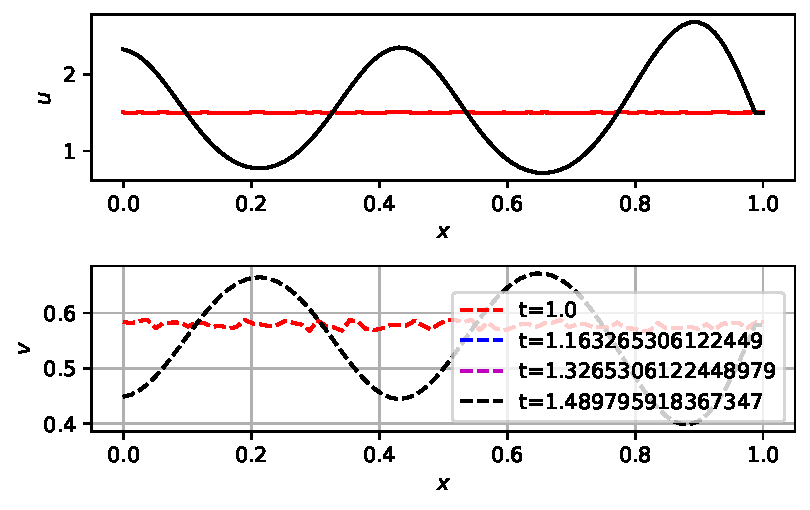
\includegraphics{DiffusionDrivenInstability_files/figure-pdf/fig-schnack_ddi_pde-output-1.pdf}

}

\caption{\label{fig-schnack_ddi_pde}DDI with Schnackenberg kinetics}

\end{figure}

In Figure Figure~\ref{fig-schnack_ddi_pde_2d} we consider a numerical
solution of the Schnackenberg model on a 2D square domain with no-flux
boundary conditions. Note

\begin{Shaded}
\begin{Highlighting}[]
\ImportTok{import}\NormalTok{ numpy }\ImportTok{as}\NormalTok{ np}
\ImportTok{from}\NormalTok{ scipy.integrate }\ImportTok{import}\NormalTok{ odeint}
\ImportTok{from}\NormalTok{ scipy.integrate }\ImportTok{import}\NormalTok{ solve\_ivp}

\ImportTok{import}\NormalTok{ matplotlib.pyplot }\ImportTok{as}\NormalTok{ plt}
\ImportTok{import}\NormalTok{ random}

\NormalTok{T}\OperatorTok{=}\DecValTok{5}
\NormalTok{L}\OperatorTok{=}\DecValTok{1}

\NormalTok{gamma}\OperatorTok{=}\FloatTok{650.0}
\NormalTok{a}\OperatorTok{=}\FloatTok{0.2}
\NormalTok{b}\OperatorTok{=}\FloatTok{1.3}
\NormalTok{d}\OperatorTok{=}\FloatTok{25.0}

\NormalTok{N\_x}\OperatorTok{=}\DecValTok{20}
\NormalTok{N\_t}\OperatorTok{=}\DecValTok{30}

\NormalTok{t}\OperatorTok{=}\NormalTok{np.linspace(}\DecValTok{1}\NormalTok{,T,N\_t)}
\NormalTok{x}\OperatorTok{=}\NormalTok{np.linspace(}\DecValTok{0}\NormalTok{,L,N\_x)}
\NormalTok{y}\OperatorTok{=}\NormalTok{np.linspace(}\DecValTok{0}\NormalTok{,L,N\_x)}

\NormalTok{[x,y]}\OperatorTok{=}\NormalTok{np.meshgrid(x,y)}

\NormalTok{u\_0}\OperatorTok{=}\NormalTok{(a}\OperatorTok{+}\NormalTok{b)}\OperatorTok{*}\NormalTok{np.ones\_like(x)}\OperatorTok{+}\FloatTok{0.01}\OperatorTok{*}\NormalTok{np.random.uniform(low}\OperatorTok{={-}}\FloatTok{1.0}\NormalTok{, high}\OperatorTok{=}\FloatTok{1.0}\NormalTok{, size}\OperatorTok{=}\NormalTok{(N\_x,N\_x))}
\NormalTok{v\_0}\OperatorTok{=}\NormalTok{b}\OperatorTok{*}\NormalTok{(}\DecValTok{1}\OperatorTok{/}\NormalTok{(a}\OperatorTok{+}\NormalTok{b)}\OperatorTok{**}\DecValTok{2}\NormalTok{)}\OperatorTok{*}\NormalTok{np.ones\_like(x)}\OperatorTok{+}\FloatTok{0.01}\OperatorTok{*}\NormalTok{np.random.uniform(low}\OperatorTok{={-}}\FloatTok{1.0}\NormalTok{, high}\OperatorTok{=}\FloatTok{1.0}\NormalTok{, size}\OperatorTok{=}\NormalTok{(N\_x,N\_x))}

\NormalTok{u\_0}\OperatorTok{=}\NormalTok{np.concatenate((np.ravel(u\_0),np.ravel(v\_0)))}

\NormalTok{dx}\OperatorTok{=}\NormalTok{L}\OperatorTok{/}\NormalTok{(N\_x}\OperatorTok{{-}}\DecValTok{1}\NormalTok{)}
\NormalTok{dt}\OperatorTok{=}\NormalTok{T}\OperatorTok{/}\NormalTok{(N\_t}\OperatorTok{{-}}\DecValTok{1}\NormalTok{)}



\KeywordTok{def}\NormalTok{ ShcnackPDErhs2d(sol,t):}

\NormalTok{    num\_nodes}\OperatorTok{=}\BuiltInTok{int}\NormalTok{(np.ceil(}\BuiltInTok{len}\NormalTok{(sol)}\OperatorTok{/}\DecValTok{2}\NormalTok{))}

\NormalTok{    u}\OperatorTok{=}\NormalTok{sol[}\DecValTok{0}\NormalTok{:num\_nodes]}
\NormalTok{    v}\OperatorTok{=}\NormalTok{sol[num\_nodes:]}


\NormalTok{    u}\OperatorTok{=}\NormalTok{np.reshape(u,(N\_x,N\_x))}
\NormalTok{    v}\OperatorTok{=}\NormalTok{np.reshape(v,(N\_x,N\_x))}

\NormalTok{    f\_u}\OperatorTok{=}\NormalTok{np.zeros\_like(u)}
\NormalTok{    f\_v}\OperatorTok{=}\NormalTok{np.zeros\_like(u)}

 

    \ControlFlowTok{for}\NormalTok{ i }\KeywordTok{in} \BuiltInTok{range}\NormalTok{(}\DecValTok{1}\NormalTok{,N\_x}\OperatorTok{{-}}\DecValTok{2}\NormalTok{):}
      \ControlFlowTok{for}\NormalTok{ j }\KeywordTok{in} \BuiltInTok{range}\NormalTok{(}\DecValTok{1}\NormalTok{,N\_x}\OperatorTok{{-}}\DecValTok{2}\NormalTok{):}
\NormalTok{        f\_u[i,j]}\OperatorTok{=}\DecValTok{1}\OperatorTok{/}\NormalTok{dx}\OperatorTok{**}\DecValTok{2}\OperatorTok{*}\NormalTok{(u[i}\OperatorTok{{-}}\DecValTok{1}\NormalTok{,j]}\OperatorTok{{-}}\DecValTok{4}\OperatorTok{*}\NormalTok{u[i,j]}\OperatorTok{+}\NormalTok{u[i}\OperatorTok{+}\DecValTok{1}\NormalTok{,j]}\OperatorTok{+}\NormalTok{u[i,j}\OperatorTok{+}\DecValTok{1}\NormalTok{]}\OperatorTok{+}\NormalTok{u[i,j}\OperatorTok{{-}}\DecValTok{1}\NormalTok{]) }
\NormalTok{        f\_v[i,j]}\OperatorTok{=}\NormalTok{d}\OperatorTok{/}\NormalTok{dx}\OperatorTok{**}\DecValTok{2}\OperatorTok{*}\NormalTok{(v[i}\OperatorTok{{-}}\DecValTok{1}\NormalTok{,j]}\OperatorTok{{-}}\DecValTok{4}\OperatorTok{*}\NormalTok{v[i,j]}\OperatorTok{+}\NormalTok{v[i}\OperatorTok{+}\DecValTok{1}\NormalTok{,j]}\OperatorTok{+}\NormalTok{v[i,j}\OperatorTok{+}\DecValTok{1}\NormalTok{]}\OperatorTok{+}\NormalTok{v[i,j}\OperatorTok{{-}}\DecValTok{1}\NormalTok{]) }

\NormalTok{    i}\OperatorTok{=}\DecValTok{0} 
    \ControlFlowTok{for}\NormalTok{ j }\KeywordTok{in} \BuiltInTok{range}\NormalTok{(}\DecValTok{1}\NormalTok{,N\_x}\OperatorTok{{-}}\DecValTok{2}\NormalTok{):}
\NormalTok{      f\_u[i,j]}\OperatorTok{=}\DecValTok{1}\OperatorTok{/}\NormalTok{dx}\OperatorTok{**}\DecValTok{2}\OperatorTok{*}\NormalTok{(}\OperatorTok{{-}}\DecValTok{3}\OperatorTok{*}\NormalTok{u[i,j]}\OperatorTok{+}\NormalTok{u[i}\OperatorTok{+}\DecValTok{1}\NormalTok{,j]}\OperatorTok{+}\NormalTok{u[i,j}\OperatorTok{+}\DecValTok{1}\NormalTok{]}\OperatorTok{+}\NormalTok{u[i,j}\OperatorTok{{-}}\DecValTok{1}\NormalTok{]) }
\NormalTok{      f\_v[i,j]}\OperatorTok{=}\NormalTok{d}\OperatorTok{/}\NormalTok{dx}\OperatorTok{**}\DecValTok{2}\OperatorTok{*}\NormalTok{(}\OperatorTok{{-}}\DecValTok{3}\OperatorTok{*}\NormalTok{v[i,j]}\OperatorTok{+}\NormalTok{v[i}\OperatorTok{+}\DecValTok{1}\NormalTok{,j]}\OperatorTok{+}\NormalTok{v[i,j}\OperatorTok{+}\DecValTok{1}\NormalTok{]}\OperatorTok{+}\NormalTok{v[i,j}\OperatorTok{{-}}\DecValTok{1}\NormalTok{]) }

\NormalTok{    i}\OperatorTok{=}\NormalTok{N\_x}\OperatorTok{{-}}\DecValTok{1}
    \ControlFlowTok{for}\NormalTok{ j }\KeywordTok{in} \BuiltInTok{range}\NormalTok{(}\DecValTok{1}\NormalTok{,N\_x}\OperatorTok{{-}}\DecValTok{2}\NormalTok{):}
\NormalTok{      f\_u[i,j]}\OperatorTok{=}\DecValTok{1}\OperatorTok{/}\NormalTok{dx}\OperatorTok{**}\DecValTok{2}\OperatorTok{*}\NormalTok{(u[i}\OperatorTok{{-}}\DecValTok{1}\NormalTok{,j]}\OperatorTok{{-}}\DecValTok{3}\OperatorTok{*}\NormalTok{u[i,j]}\OperatorTok{+}\NormalTok{u[i,j}\OperatorTok{+}\DecValTok{1}\NormalTok{]}\OperatorTok{+}\NormalTok{u[i,j}\OperatorTok{{-}}\DecValTok{1}\NormalTok{]) }
\NormalTok{      f\_v[i,j]}\OperatorTok{=}\NormalTok{d}\OperatorTok{/}\NormalTok{dx}\OperatorTok{**}\DecValTok{2}\OperatorTok{*}\NormalTok{(v[i}\OperatorTok{{-}}\DecValTok{1}\NormalTok{,j]}\OperatorTok{{-}}\DecValTok{3}\OperatorTok{*}\NormalTok{v[i,j]}\OperatorTok{+}\NormalTok{v[i,j}\OperatorTok{+}\DecValTok{1}\NormalTok{]}\OperatorTok{+}\NormalTok{v[i,j}\OperatorTok{{-}}\DecValTok{1}\NormalTok{])   }

\NormalTok{    j}\OperatorTok{=}\DecValTok{0}
    \ControlFlowTok{for}\NormalTok{ i }\KeywordTok{in} \BuiltInTok{range}\NormalTok{(}\DecValTok{1}\NormalTok{,N\_x}\OperatorTok{{-}}\DecValTok{2}\NormalTok{):}
\NormalTok{        f\_u[i,j]}\OperatorTok{=}\DecValTok{1}\OperatorTok{/}\NormalTok{dx}\OperatorTok{**}\DecValTok{2}\OperatorTok{*}\NormalTok{(u[i}\OperatorTok{{-}}\DecValTok{1}\NormalTok{,j]}\OperatorTok{{-}}\DecValTok{3}\OperatorTok{*}\NormalTok{u[i,j]}\OperatorTok{+}\NormalTok{u[i}\OperatorTok{+}\DecValTok{1}\NormalTok{,j]}\OperatorTok{+}\NormalTok{u[i,j}\OperatorTok{+}\DecValTok{1}\NormalTok{]) }
\NormalTok{        f\_v[i,j]}\OperatorTok{=}\NormalTok{d}\OperatorTok{/}\NormalTok{dx}\OperatorTok{**}\DecValTok{2}\OperatorTok{*}\NormalTok{(v[i}\OperatorTok{{-}}\DecValTok{1}\NormalTok{,j]}\OperatorTok{{-}}\DecValTok{3}\OperatorTok{*}\NormalTok{v[i,j]}\OperatorTok{+}\NormalTok{v[i}\OperatorTok{+}\DecValTok{1}\NormalTok{,j]}\OperatorTok{+}\NormalTok{v[i,j}\OperatorTok{+}\DecValTok{1}\NormalTok{]) }

\NormalTok{    j }\OperatorTok{=}\NormalTok{N\_x}\OperatorTok{{-}}\DecValTok{1}
    \ControlFlowTok{for}\NormalTok{ i }\KeywordTok{in} \BuiltInTok{range}\NormalTok{(}\DecValTok{1}\NormalTok{,N\_x}\OperatorTok{{-}}\DecValTok{2}\NormalTok{):}
\NormalTok{        f\_u[i,j]}\OperatorTok{=}\DecValTok{1}\OperatorTok{/}\NormalTok{dx}\OperatorTok{**}\DecValTok{2}\OperatorTok{*}\NormalTok{(u[i}\OperatorTok{{-}}\DecValTok{1}\NormalTok{,j]}\OperatorTok{{-}}\DecValTok{3}\OperatorTok{*}\NormalTok{u[i,j]}\OperatorTok{+}\NormalTok{u[i}\OperatorTok{+}\DecValTok{1}\NormalTok{,j]}\OperatorTok{+}\NormalTok{u[i,j}\OperatorTok{{-}}\DecValTok{1}\NormalTok{]) }
\NormalTok{        f\_v[i,j]}\OperatorTok{=}\NormalTok{d}\OperatorTok{/}\NormalTok{dx}\OperatorTok{**}\DecValTok{2}\OperatorTok{*}\NormalTok{(v[i}\OperatorTok{{-}}\DecValTok{1}\NormalTok{,j]}\OperatorTok{{-}}\DecValTok{3}\OperatorTok{*}\NormalTok{v[i,j]}\OperatorTok{+}\NormalTok{v[i}\OperatorTok{+}\DecValTok{1}\NormalTok{,j]}\OperatorTok{+}\NormalTok{v[i,j}\OperatorTok{{-}}\DecValTok{1}\NormalTok{])  }

\NormalTok{    i}\OperatorTok{=}\DecValTok{0}
\NormalTok{    j}\OperatorTok{=}\DecValTok{0}
\NormalTok{    f\_u[i,j]}\OperatorTok{=}\DecValTok{1}\OperatorTok{/}\NormalTok{dx}\OperatorTok{**}\DecValTok{2}\OperatorTok{*}\NormalTok{(}\OperatorTok{{-}}\DecValTok{2}\OperatorTok{*}\NormalTok{u[i,j]}\OperatorTok{+}\NormalTok{u[i}\OperatorTok{+}\DecValTok{1}\NormalTok{,j]}\OperatorTok{+}\NormalTok{u[i,j}\OperatorTok{+}\DecValTok{1}\NormalTok{]) }
\NormalTok{    f\_v[i,j]}\OperatorTok{=}\NormalTok{d}\OperatorTok{/}\NormalTok{dx}\OperatorTok{**}\DecValTok{2}\OperatorTok{*}\NormalTok{(}\OperatorTok{{-}}\DecValTok{2}\OperatorTok{*}\NormalTok{v[i,j]}\OperatorTok{+}\NormalTok{v[i}\OperatorTok{+}\DecValTok{1}\NormalTok{,j]}\OperatorTok{+}\NormalTok{v[i,j}\OperatorTok{+}\DecValTok{1}\NormalTok{]) }

\NormalTok{    i}\OperatorTok{=}\DecValTok{0}
\NormalTok{    j}\OperatorTok{=}\NormalTok{N\_x}\OperatorTok{{-}}\DecValTok{1}
\NormalTok{    f\_u[i,j]}\OperatorTok{=}\DecValTok{1}\OperatorTok{/}\NormalTok{dx}\OperatorTok{**}\DecValTok{2}\OperatorTok{*}\NormalTok{(}\OperatorTok{{-}}\DecValTok{2}\OperatorTok{*}\NormalTok{u[i,j]}\OperatorTok{+}\NormalTok{u[i}\OperatorTok{+}\DecValTok{1}\NormalTok{,j]}\OperatorTok{+}\NormalTok{u[i,j}\OperatorTok{{-}}\DecValTok{1}\NormalTok{]) }
\NormalTok{    f\_v[i,j]}\OperatorTok{=}\NormalTok{d}\OperatorTok{/}\NormalTok{dx}\OperatorTok{**}\DecValTok{2}\OperatorTok{*}\NormalTok{(}\OperatorTok{{-}}\DecValTok{2}\OperatorTok{*}\NormalTok{v[i,j]}\OperatorTok{+}\NormalTok{v[i}\OperatorTok{+}\DecValTok{1}\NormalTok{,j]}\OperatorTok{+}\NormalTok{v[i,j}\OperatorTok{{-}}\DecValTok{1}\NormalTok{]) }

\NormalTok{    i}\OperatorTok{=}\NormalTok{N\_x}\OperatorTok{{-}}\DecValTok{1}
\NormalTok{    j}\OperatorTok{=}\DecValTok{0}

\NormalTok{    f\_u[i,j]}\OperatorTok{=}\DecValTok{1}\OperatorTok{/}\NormalTok{dx}\OperatorTok{**}\DecValTok{2}\OperatorTok{*}\NormalTok{(u[i}\OperatorTok{{-}}\DecValTok{1}\NormalTok{,j]}\OperatorTok{{-}}\DecValTok{2}\OperatorTok{*}\NormalTok{u[i,j]}\OperatorTok{+}\NormalTok{u[i,j}\OperatorTok{+}\DecValTok{1}\NormalTok{]) }
\NormalTok{    f\_v[i,j]}\OperatorTok{=}\NormalTok{d}\OperatorTok{/}\NormalTok{dx}\OperatorTok{**}\DecValTok{2}\OperatorTok{*}\NormalTok{(v[i}\OperatorTok{{-}}\DecValTok{1}\NormalTok{,j]}\OperatorTok{{-}}\DecValTok{2}\OperatorTok{*}\NormalTok{v[i,j]}\OperatorTok{+}\NormalTok{v[i,j}\OperatorTok{+}\DecValTok{1}\NormalTok{]) }
    
\NormalTok{    i}\OperatorTok{=}\NormalTok{N\_x}\OperatorTok{{-}}\DecValTok{1}
\NormalTok{    j}\OperatorTok{=}\NormalTok{N\_x}\OperatorTok{{-}}\DecValTok{1}


\NormalTok{    f\_u[i,j]}\OperatorTok{=}\DecValTok{1}\OperatorTok{/}\NormalTok{dx}\OperatorTok{**}\DecValTok{2}\OperatorTok{*}\NormalTok{(}\OperatorTok{{-}}\DecValTok{2}\OperatorTok{*}\NormalTok{u[i,j]}\OperatorTok{+}\NormalTok{u[i}\OperatorTok{{-}}\DecValTok{1}\NormalTok{,j]}\OperatorTok{+}\NormalTok{u[i,j}\OperatorTok{{-}}\DecValTok{1}\NormalTok{]) }
\NormalTok{    f\_v[i,j]}\OperatorTok{=}\NormalTok{d}\OperatorTok{/}\NormalTok{dx}\OperatorTok{**}\DecValTok{2}\OperatorTok{*}\NormalTok{(}\OperatorTok{{-}}\DecValTok{2}\OperatorTok{*}\NormalTok{v[i,j]}\OperatorTok{+}\NormalTok{v[i}\OperatorTok{{-}}\DecValTok{1}\NormalTok{,j]}\OperatorTok{+}\NormalTok{v[i,j}\OperatorTok{{-}}\DecValTok{1}\NormalTok{]) }


\NormalTok{    reaction\_u}\OperatorTok{=}\NormalTok{gamma}\OperatorTok{*}\NormalTok{(a}\OperatorTok{{-}}\NormalTok{u}\OperatorTok{+}\NormalTok{(u}\OperatorTok{**}\DecValTok{2}\NormalTok{)}\OperatorTok{*}\NormalTok{v)}
\NormalTok{    reaction\_v}\OperatorTok{=}\NormalTok{gamma}\OperatorTok{*}\NormalTok{(b}\OperatorTok{{-}}\NormalTok{(u}\OperatorTok{**}\DecValTok{2}\NormalTok{)}\OperatorTok{*}\NormalTok{v)}

\NormalTok{    f\_u}\OperatorTok{=}\NormalTok{f\_u}\OperatorTok{+}\NormalTok{reaction\_u}
\NormalTok{    f\_v}\OperatorTok{=}\NormalTok{f\_v}\OperatorTok{+}\NormalTok{reaction\_v}



\NormalTok{    f}\OperatorTok{=}\NormalTok{ np.concatenate((np.ravel(f\_u),np.ravel(f\_v))) }
    \ControlFlowTok{return}\NormalTok{ f  }

\NormalTok{sol}\OperatorTok{=}\NormalTok{odeint(ShcnackPDErhs2d,u\_0,t)}
\CommentTok{\#soln = solve\_ivp(ShcnackPDErhs,(0, T), u\_0, method=\textquotesingle{}Radau\textquotesingle{})}


\NormalTok{u\_0}\OperatorTok{=}\NormalTok{sol[}\DecValTok{0}\NormalTok{,}\DecValTok{0}\NormalTok{:N\_x}\OperatorTok{**}\DecValTok{2}\NormalTok{]}
\NormalTok{v\_0}\OperatorTok{=}\NormalTok{sol[}\DecValTok{0}\NormalTok{,N\_x}\OperatorTok{**}\DecValTok{2}\NormalTok{:]}
\NormalTok{u\_0}\OperatorTok{=}\NormalTok{np.reshape(u\_0,(N\_x,N\_x))}
\NormalTok{v\_0}\OperatorTok{=}\NormalTok{np.reshape(v\_0,(N\_x,N\_x))}

\NormalTok{u\_m}\OperatorTok{=}\NormalTok{sol[}\DecValTok{20}\NormalTok{,}\DecValTok{0}\NormalTok{:N\_x}\OperatorTok{**}\DecValTok{2}\NormalTok{]}
\NormalTok{v\_m}\OperatorTok{=}\NormalTok{sol[}\DecValTok{20}\NormalTok{,N\_x}\OperatorTok{**}\DecValTok{2}\NormalTok{:]}
\NormalTok{u\_m}\OperatorTok{=}\NormalTok{np.reshape(u\_m,(N\_x,N\_x))}
\NormalTok{v\_m}\OperatorTok{=}\NormalTok{np.reshape(v\_m,(N\_x,N\_x))}

\NormalTok{u}\OperatorTok{=}\NormalTok{sol[}\OperatorTok{{-}}\DecValTok{1}\NormalTok{,}\DecValTok{0}\NormalTok{:N\_x}\OperatorTok{**}\DecValTok{2}\NormalTok{]}
\NormalTok{v}\OperatorTok{=}\NormalTok{sol[}\OperatorTok{{-}}\DecValTok{1}\NormalTok{,N\_x}\OperatorTok{**}\DecValTok{2}\NormalTok{:]}
\NormalTok{u}\OperatorTok{=}\NormalTok{np.reshape(u,(N\_x,N\_x))}
\NormalTok{v}\OperatorTok{=}\NormalTok{np.reshape(v,(N\_x,N\_x))}

\NormalTok{fig, ax }\OperatorTok{=}\NormalTok{ plt.subplots(}\DecValTok{2}\NormalTok{,}\DecValTok{3}\NormalTok{)}
\NormalTok{ax[}\DecValTok{0}\NormalTok{,}\DecValTok{0}\NormalTok{].imshow(u\_0)}
\NormalTok{ax[}\DecValTok{1}\NormalTok{,}\DecValTok{0}\NormalTok{].imshow(v\_0)}
\NormalTok{ax[}\DecValTok{0}\NormalTok{,}\DecValTok{1}\NormalTok{].imshow(u\_m)}
\NormalTok{ax[}\DecValTok{1}\NormalTok{,}\DecValTok{1}\NormalTok{].imshow(v\_m)}
\NormalTok{ax[}\DecValTok{0}\NormalTok{,}\DecValTok{2}\NormalTok{].imshow(u)}
\NormalTok{ax[}\DecValTok{1}\NormalTok{,}\DecValTok{2}\NormalTok{].imshow(v)}

\CommentTok{\textquotesingle{}\textquotesingle{}\textquotesingle{}}
\CommentTok{ax[0].plot(x,u[0,:],\textquotesingle{}r\textquotesingle{})}
\CommentTok{ax[0].plot(x,u[16,:],\textquotesingle{}b\textquotesingle{})}
\CommentTok{ax[0].plot(x,u[32,:],\textquotesingle{}m\textquotesingle{})}
\CommentTok{ax[0].plot(x,u[48,:],\textquotesingle{}k\textquotesingle{})}
\CommentTok{ax[0].set\_xlabel(\textquotesingle{}$x$\textquotesingle{})}
\CommentTok{ax[0].set\_ylabel(\textquotesingle{}$u$\textquotesingle{})}

\CommentTok{ax[1].plot(x, v[0,:],\textquotesingle{}r{-}{-}\textquotesingle{})}
\CommentTok{ax[1].plot(x, v[16,:],\textquotesingle{}b{-}{-}\textquotesingle{})}
\CommentTok{ax[1].plot(x, v[32,:],\textquotesingle{}m{-}{-}\textquotesingle{})}
\CommentTok{ax[1].plot(x, v[48,:],\textquotesingle{}k{-}{-}\textquotesingle{})}
\CommentTok{ax[1].set\_xlabel(\textquotesingle{}$x$\textquotesingle{})}
\CommentTok{ax[1].set\_ylabel(\textquotesingle{}$v$\textquotesingle{})}
\CommentTok{\textquotesingle{}\textquotesingle{}\textquotesingle{}}

\NormalTok{plt.xlabel(}\StringTok{\textquotesingle{}$x$\textquotesingle{}}\NormalTok{)}
\NormalTok{plt.show()}
\end{Highlighting}
\end{Shaded}

\begin{figure}[H]

{\centering 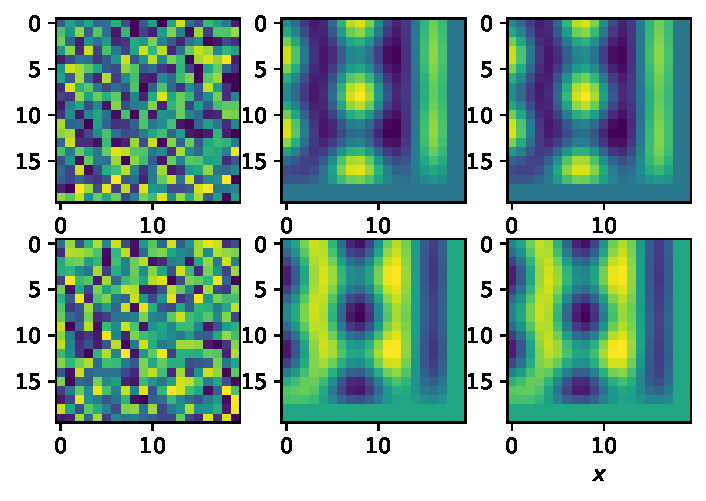
\includegraphics{DiffusionDrivenInstability_files/figure-pdf/fig-schnack_ddi_pde_2d-output-1.pdf}

}

\caption{\label{fig-schnack_ddi_pde_2d}DDI with Schnackenberg kinetics
in 2D}

\end{figure}

\hypertarget{linear-stability-analysis-and-evolution-of-spatial-pattern-general-conditions-for-diffusion-driven-instability}{%
\section{Linear Stability Analysis and Evolution of Spatial Pattern:
General Conditions for Diffusion-driven
Instability}\label{linear-stability-analysis-and-evolution-of-spatial-pattern-general-conditions-for-diffusion-driven-instability}}

Let \(\Omega\subset \mathbb R^n\) be a domain with smooth (sufficiently
regular) boundary \(\partial \Omega\), with outward unit normal
\({\mathbf{n}}\). Our general, non-dimensional reaction-diffusion system
is then:

\begin{equation}\protect\hypertarget{eq-pp}{}{
\begin{aligned}
&\frac{\partial u}{\partial  t} = \gamma\, f(u,v)  +  \nabla^2 u, \qquad x\in \Omega, \quad t>0, \\
&\frac{\partial v}{\partial  t} = \gamma\, g(u,v)  + d \nabla^2 v, \qquad x\in \Omega, \quad t>0, \\
&
\end{aligned}
}\label{eq-pp}\end{equation} together with boundary and initial
Conditions \begin{equation}\protect\hypertarget{eq-pp_bc}{}{
\begin{aligned}
\nabla u \cdot {\mathbf{n} } = 0, \qquad \nabla v \cdot {\mathbf{n} } = 0, \qquad x\in \partial \Omega, \quad t>0, \\
u(x,0)  = u_0(x), \qquad  v(x,0)  = v_0(x), \qquad x\in \Omega\; .
\end{aligned}
}\label{eq-pp_bc}\end{equation}

A \textbf{spatially homogeneous steady-state} of Equation~\ref{eq-pp}
and Equation~\ref{eq-pp_bc} satisfies \[
f(u,v) = 0 , \qquad g(u,v) =0
\] and we denote it by \((u_0, v_0)\).

\hypertarget{stability-of-spatially-homogeneous-steady-states-to-spatially-homogeneous-perturbations}{%
\subsection{Stability of spatially homogeneous steady states to
spatially homogeneous
perturbations}\label{stability-of-spatially-homogeneous-steady-states-to-spatially-homogeneous-perturbations}}

Before we consider the effect of the spatial terms (i.e.~diffusion) in
Equation~\ref{eq-pp} and Equation~\ref{eq-pp_bc}, we first of all
explore the stability of the underlying spatially homogeneous steady
state.

Consider the following perturbations to the steady state
\((u_0 , v_0)\): \[
u(x,t) = u_0 + \tilde u(t), \quad  v(x,t) = v_0 + \tilde v(t), \qquad \|\tilde u(t) \| \ll 1, \quad  \|\tilde v(t) \| \ll 1.
\]

Upon substitution into Equation~\ref{eq-pp}
\begin{equation}\protect\hypertarget{eq-pp_1}{}{
\begin{aligned}
\frac{d\tilde u}{d t} = \gamma\, f(u_0 + \tilde u,v_0 + \tilde v),  \\
\frac{d \tilde v}{d  t} = \gamma\, g(u_0 + \tilde u,v_0 + \tilde v).
\end{aligned}
}\label{eq-pp_1}\end{equation}

Using a Taylor expansion of \(f\) and \(g\) about \((u_0, v_0)\) we
obtain the linearised system
\begin{equation}\protect\hypertarget{eq-linear_pp}{}{
\begin{pmatrix} 
\tilde u_t \\
\tilde v_t
\end{pmatrix}  = \gamma J  \begin{pmatrix} 
\tilde u \\
\tilde v
\end{pmatrix},
}\label{eq-linear_pp}\end{equation} where \[
J =J(u_0, v_0) =  \begin{pmatrix} 
f_u & f_v  \\
g_u & g_v 
\end{pmatrix}_{(u_0 , v_0)} \; .  
\]

The general solution of Equation~\ref{eq-linear_pp} is

\[
 \begin{pmatrix} 
\tilde u(t) \\
\tilde v(t)
\end{pmatrix}   =  C_1 \phi_1 e^{\lambda_1 t} +  C_2 \phi_2 e^{\lambda_2 t}  , 
\] where \(C_1\), \(C_2\) are arbitrary constants,
\(\lambda_1, \lambda_2\) are the eigenvalues of \(\gamma J\),
i.e.~solutions of characteristic equation \[
\det (\gamma J - \lambda I) = 0,
\] and \(\phi_1\), \(\phi_2\) are corresponding eigenvectors. It is
easily seen that

\[
\lambda_{1,2} = \frac \gamma 2 \left( \text{tr} (J) \pm \sqrt{ \text{tr}(J)^2 - 4 \det(J)} \right),
\]

and thus a spatially homogeneous steady state \((u_0, v_0)\) is
\textbf{stable} to spatially homogeneous perturbations if \[
{\mathrm Re}( \lambda_{1,2}) <0,
\] i.e.~if

\begin{equation}\protect\hypertarget{eq-stable_hom}{}{
\begin{aligned}
\text{tr}(J) & = f_u + g_v < 0, \\
\det(J) & = f_u g_v - f_v g_u > 0. 
\end{aligned}
}\label{eq-stable_hom}\end{equation}

We shall be interested only in such parameter values for which
conditions Equation~\ref{eq-stable_hom} are satisfied (i.e.~the
spatially homogeneous steady state is linearly stable in the absence of
diffusion).

\hypertarget{stability-of-spatially-homogeneous-steady-states-to-spatially-heterogeneous-spatially-dependent-perturbations}{%
\subsection{Stability of spatially homogeneous steady states to
spatially heterogeneous: spatially dependent,
perturbations}\label{stability-of-spatially-homogeneous-steady-states-to-spatially-heterogeneous-spatially-dependent-perturbations}}

We now consider perturbations about the spatially homogeneous steady
state that are spatially dependent i.e.~ \[
u(x,t) = u_0 + \tilde u(x,t), \quad  v(x,t) = v_0 + \tilde v(x,t), \qquad \|\tilde u(x,t) \| \ll 1, \quad  \|\tilde v(x,t) \| \ll 1 .
\]

Upon substitution in Equation~\ref{eq-pp} and apply a Taylor expansion
about \((u_0, v_0)\) to \(f\) and \(g\) to obtain the linearised problem

\begin{equation}\protect\hypertarget{eq-pp_3}{}{
\begin{aligned}
\frac{\partial \tilde u(x,t)}{\partial t} = \gamma\, \left(f_u \tilde u(x,t) + f_v \tilde v(x,t)\right) + \nabla^2 \tilde u(x,t)  , \quad x\in \Omega, \;  t >0, \\
\frac{\partial \tilde v(x,t)}{\partial   t} = \gamma\,  \left(g_u  \tilde u(x,t) + g_v \tilde v(x,t)\right) +d \nabla^2 \tilde v(x,t)  ,  \quad x\in \Omega, \;  t >0,  \\
\end{aligned}
}\label{eq-pp_3}\end{equation} with boundary conditions
\begin{equation}\protect\hypertarget{eq-pp_3bc}{}{
\begin{aligned}
{\mathbf{n}} \cdot \nabla \tilde u (x,t) = 0, \qquad {\mathbf{n}} \cdot \nabla \tilde v (x,t)  = 0, \qquad   x\in   \partial \Omega, \; t >0.
\end{aligned}
}\label{eq-pp_3bc}\end{equation}

Defining \[
V(x,t) = \begin{pmatrix} 
\tilde u(x,t) \\
\tilde v(x,t)
\end{pmatrix}
\] we rewrite Equation~\ref{eq-pp_3} as \[
\frac{\partial}{\partial t}  V(x,t) = \gamma J  V(x,t) + D \nabla^2   V(x,t), 
\]

where

\[
D =  \begin{pmatrix} 
1 & 0 \\
0 & d 
\end{pmatrix}\;.
\]

We shall consider a separation of variables approach, i.e. \[
V(x,t) =\begin{pmatrix}  
 \bar u(t)  \varphi_1(x)
 \\
 \bar v(t)  \varphi_2(x)
 \end{pmatrix}\;
\] and obtain \begin{equation}\protect\hypertarget{eq-pp_4}{}{
\begin{aligned}
\frac{d \bar u(t)}{d t}\varphi_1(x) = \gamma\, \left(f_u \bar u(t) \varphi_1(x) + f_v \bar v(t) \varphi_2(x)\right) +\bar u(t)  \nabla^2 \varphi_1(x)  , \quad x\in \Omega, \;  t >0, \\
\frac{d \bar v(t)}{d t}\varphi_2(x) = \gamma\,  \left(g_u  \bar u(t) \varphi_1(x) + g_v \bar v(t) \varphi_2(x)\right) +  d \bar v(t) \nabla^2  \varphi_2(x)  ,  \quad x\in \Omega, \;  t >0,  \\
\end{aligned}
}\label{eq-pp_4}\end{equation}

with boundary conditions
\begin{equation}\protect\hypertarget{eq-pp_4bc}{}{
\begin{aligned}
{\mathbf{n}} \cdot \nabla \varphi_1(x) = 0, \qquad {\mathbf{n}} \cdot \nabla\varphi_2 (x) = 0, \qquad   x\in   \partial \Omega, \; t >0.
\end{aligned}
}\label{eq-pp_4bc}\end{equation}

It is assumed that \[
\bar u(t)\, / \hspace{-0.35 cm}\equiv 0 \quad \textrm{and} \quad  \bar v(t)\, / \hspace{-0.35 cm}\equiv 0
\] for \(t>0\).

\begin{lemma}[]\protect\hypertarget{lem-laplacianeiegenvalues}{}\label{lem-laplacianeiegenvalues}

Consider the spatial eigenvalue problem for the Laplacian \(\nabla^2\)
with zero-Neumann boundary conditions i.e.

\begin{equation}\protect\hypertarget{eq-ev}{}{
\begin{aligned}
\nabla^2 \psi(x) = -k^2 \psi(x) , \qquad x \in \Omega ,  \\
{\mathbf{n}} \cdot \nabla \psi(x) = 0 , \qquad x\in \partial \Omega \; . 
\end{aligned}
}\label{eq-ev}\end{equation}

For a bounded domain \(\Omega\) there exists a discrete set of
eigenvalues \[
0 \leq k^2_1< k_2^2\leq k_3^2\leq \ldots \leq k_j^2\leq \ldots,
\] with \[
j \in \mathbb N, \quad  \textrm{and} \quad k_j^2 \to \infty \quad \textrm{as}  \quad j \to \infty.
\]

Moreover, the eigenfunctions \(\{\psi_k(x) \}\) form an
\textbf{orthogonal set} of basis functions of the corresponding
functional space (i.e.~\(L^2(\Omega)\), \(H^1(\Omega)\)).

\end{lemma}

Thus we can look for the spatial component of the solution of
Equation~\ref{eq-pp_4} as follows: \[
\varphi(x) = \begin{pmatrix}  
\varphi_1(x) \\
\varphi_2(x)
 \end{pmatrix} = \sum_k C_k \psi_k(x), \qquad C_k =  \begin{pmatrix}  C_k^1 \\ C_k^2 \end{pmatrix} \in \mathbb R^2 \; 
\] and \begin{equation}\protect\hypertarget{eq-vxt}{}{
\begin{aligned}
V(x,t) =\sum_k \hat V_k(t) \psi_k(x), \qquad \textrm{ where} 
\quad \hat V_k(t)=
\begin{pmatrix}  
C_k^1 \; \bar u(t) 
 \\
 C_k^2 \; \bar v(t) 
 \end{pmatrix}.
\end{aligned}
}\label{eq-vxt}\end{equation}

SEince \(\nabla^2 \psi_k(x) = - k^2 \psi_k(x)\) we obtain

\[
D \nabla^2  V(x,t) = D \nabla^2 \left[ \sum_k \hat V_k(t) \psi_k(x) \right]   = \sum_k D \hat V_k(t) \nabla^2 \psi_k(x)= 
- \sum_k k^2 D \hat V_k(t)  \psi_k(x).
\]

Hence

\[
\sum_k \frac{d}{d t}  \hat V_k(t) \psi_k(x)  =
  \sum_k \gamma J \hat V_k(t) \psi_k(x) -  \sum_k k^2  D \hat V_k(t) \psi_k(x). 
\]

Since \(\{\psi_k(x) \}\) is a orthogonal basis we obtain that

\[
 \frac{d}{d t}  \hat V_k(t) \psi_k(x)  =
   \gamma J  \hat V_k(t) \psi_k(x) -  k^2  D \hat V_k(t) \psi_k(x), 
\] for each \(k\). Finally, since \[
\psi_k(x)\;  /\hspace{-0.35 cm }\equiv 0
\] in \(\Omega\) this implies for each \(k\) a system of ODEs:

\begin{equation}\protect\hypertarget{eq-stab_pp_ode}{}{
\begin{aligned}
 \frac{d}{d t}  \hat V_k(t)   &=   \left(\gamma J  -  k^2  D\right) \hat V_k(t) &= \tilde J\hat V_k(t) ,
\end{aligned}
}\label{eq-stab_pp_ode}\end{equation}

where \(\tilde J\) is a ``modified'' Jacobian:

\[
\tilde{J} =  \begin{pmatrix} 
\gamma f_u - k^2 & \gamma f_v \\
\gamma g_u & \gamma g_v - d k^2
\end{pmatrix}\;.
\]

Now solutions of Equation~\ref{eq-stab_pp_ode} are of the form \[
\hat V_k(t) = e^{\lambda t} P_k
\] with \(P_k \in \mathbb R^2\), where, since \(P_k\neq 0\) (looking for
nontrivial solutions), we find that \(\lambda\) are the eigenvalues of
\(\tilde J\) , i.e.~

solutions of the characteristic equation
\begin{equation}\protect\hypertarget{eq-charact_pp_1}{}{
\det(\tilde J - \lambda I) = \det ( \gamma J - k^2 D - \lambda I) =0. 
}\label{eq-charact_pp_1}\end{equation}

Evaluating the above determinant, we arrive at the equation:
\begin{equation}\protect\hypertarget{eq-spatial_eigenvalues}{}{
\lambda^2 + [ k^2 (1 + d) - \gamma (f_u + g_v) ] \lambda + h(k^2) = 0,
}\label{eq-spatial_eigenvalues}\end{equation} where
\begin{equation}\protect\hypertarget{eq-hk2}{}{
h(k^2) = dk^4 - \gamma (df_u + g_v) k^2 + \gamma^2 | J | .
}\label{eq-hk2}\end{equation}

\begin{figure}

{\centering 

\begin{Shaded}
\begin{Highlighting}[]
\ImportTok{import}\NormalTok{ numpy }\ImportTok{as}\NormalTok{ np}
\ImportTok{import}\NormalTok{ matplotlib.pyplot }\ImportTok{as}\NormalTok{ plt}

\CommentTok{\# genera}
\NormalTok{k\_sq}\OperatorTok{=}\NormalTok{np.linspace(}\DecValTok{0}\NormalTok{,}\DecValTok{25}\NormalTok{,}\DecValTok{100}\NormalTok{)}


\NormalTok{gamma}\OperatorTok{=}\DecValTok{10}
\NormalTok{d\_1}\OperatorTok{=}\FloatTok{0.02}
\NormalTok{d\_2}\OperatorTok{=}\DecValTok{3}
\NormalTok{d\_3}\OperatorTok{=}\DecValTok{6}


\NormalTok{f\_u}\OperatorTok{=}\FloatTok{0.2}
\NormalTok{g\_v}\OperatorTok{={-}}\FloatTok{0.5}
\NormalTok{term1}\OperatorTok{=}\NormalTok{d}\OperatorTok{*}\NormalTok{f\_u}\OperatorTok{+}\NormalTok{g\_v}
\NormalTok{J}\OperatorTok{=}\FloatTok{1.0} \CommentTok{\# positive determinant}



\KeywordTok{def}\NormalTok{ Computeh(k\_sq,d):}
\NormalTok{  h}\OperatorTok{=}\NormalTok{d}\OperatorTok{*}\NormalTok{k\_sq}\OperatorTok{**}\DecValTok{2}\OperatorTok{{-}}\NormalTok{gamma}\OperatorTok{*}\NormalTok{(term1)}\OperatorTok{*}\NormalTok{k\_sq}\OperatorTok{+}\NormalTok{ gamma}\OperatorTok{**}\DecValTok{2}\OperatorTok{*}\NormalTok{J}
  \ControlFlowTok{return}\NormalTok{ h}

\KeywordTok{def}\NormalTok{ SolveReLambda(k\_sq,d):}
   \CommentTok{\# a lam\^{}2 + b * lam +c}
\NormalTok{    a}\OperatorTok{=}\DecValTok{1}
\NormalTok{    b}\OperatorTok{=}\NormalTok{ k\_sq}\OperatorTok{*}\NormalTok{(}\DecValTok{1}\OperatorTok{+}\NormalTok{d)}\OperatorTok{{-}}\NormalTok{gamma}\OperatorTok{*}\NormalTok{(f\_u}\OperatorTok{+}\NormalTok{g\_v)}
\NormalTok{    c}\OperatorTok{=}\NormalTok{ Computeh(k\_sq,d)}
\NormalTok{    lambda\_m}\OperatorTok{=}\NormalTok{ (}\OperatorTok{{-}}\NormalTok{b}\OperatorTok{{-}}\NormalTok{np.sqrt(b}\OperatorTok{**}\DecValTok{2}\OperatorTok{{-}}\DecValTok{4}\OperatorTok{*}\NormalTok{a}\OperatorTok{*}\NormalTok{c))}\OperatorTok{/}\NormalTok{(}\DecValTok{2}\OperatorTok{*}\NormalTok{a)}
\NormalTok{    lambda\_p}\OperatorTok{=}\NormalTok{ (}\OperatorTok{{-}}\NormalTok{b}\OperatorTok{+}\NormalTok{np.sqrt(b}\OperatorTok{**}\DecValTok{2}\OperatorTok{{-}}\DecValTok{4}\OperatorTok{*}\NormalTok{a}\OperatorTok{*}\NormalTok{c))}\OperatorTok{//}\NormalTok{(}\DecValTok{2}\OperatorTok{*}\NormalTok{a)}
    \ControlFlowTok{return}\NormalTok{ lambda\_m,lambda\_p}

\KeywordTok{def}\NormalTok{ TestDDIconditions(d):}

\NormalTok{    cond\_1}\OperatorTok{=}\NormalTok{f\_u}\OperatorTok{+}\NormalTok{g\_v}
\NormalTok{    cond\_2 }\OperatorTok{=}\NormalTok{ J}
\NormalTok{    cond\_3 }\OperatorTok{=}\NormalTok{ d}\OperatorTok{*}\NormalTok{f\_u}\OperatorTok{+}\NormalTok{g\_v}
\NormalTok{    cond\_4 }\OperatorTok{=}\NormalTok{ (d}\OperatorTok{*}\NormalTok{f\_u}\OperatorTok{+}\NormalTok{g\_v)}\OperatorTok{**}\DecValTok{2}\OperatorTok{{-}}\DecValTok{4}\OperatorTok{*}\NormalTok{d}\OperatorTok{*}\NormalTok{J}

\NormalTok{    cond\_true}\OperatorTok{=}\NormalTok{np.zeros((}\DecValTok{4}\NormalTok{,}\DecValTok{1}\NormalTok{),dtype}\OperatorTok{=}\BuiltInTok{bool}\NormalTok{)}
\NormalTok{    cond\_true[}\DecValTok{0}\NormalTok{]}\OperatorTok{=}\NormalTok{(cond\_1}\OperatorTok{\textless{}}\DecValTok{0}\NormalTok{) }
\NormalTok{    cond\_true[}\DecValTok{1}\NormalTok{]}\OperatorTok{=}\NormalTok{ (cond\_2}\OperatorTok{\textgreater{}}\DecValTok{0}\NormalTok{) }
\NormalTok{    cond\_true[}\DecValTok{2}\NormalTok{]}\OperatorTok{=}\NormalTok{ (cond\_3}\OperatorTok{\textgreater{}}\DecValTok{0}\NormalTok{)}
\NormalTok{    cond\_true[}\DecValTok{3}\NormalTok{]}\OperatorTok{=}\NormalTok{(cond\_4}\OperatorTok{\textless{}}\DecValTok{0}\NormalTok{)}


    \ControlFlowTok{return}\NormalTok{ cond\_true}

\NormalTok{h\_1}\OperatorTok{=}\NormalTok{Computeh(k\_sq,d\_1)}
\NormalTok{h\_2}\OperatorTok{=}\NormalTok{Computeh(k\_sq,d\_2)}
\NormalTok{h\_3}\OperatorTok{=}\NormalTok{Computeh(k\_sq,d\_3)}

\NormalTok{l\_1\_m, l\_1\_p }\OperatorTok{=}\NormalTok{ SolveReLambda(k\_sq,d\_1)}
\NormalTok{l\_2\_m, l\_2\_p }\OperatorTok{=}\NormalTok{ SolveReLambda(k\_sq,d\_2)}
\NormalTok{l\_3\_m, l\_3\_p }\OperatorTok{=}\NormalTok{ SolveReLambda(k\_sq,d\_3)}

\NormalTok{conditions\_satisfied1}\OperatorTok{=}\NormalTok{TestDDIconditions(d\_1)}
\NormalTok{conditions\_satisfied2}\OperatorTok{=}\NormalTok{TestDDIconditions(d\_2)}
\NormalTok{conditions\_satisfied3}\OperatorTok{=}\NormalTok{TestDDIconditions(d\_3)}

\BuiltInTok{print}\NormalTok{(conditions\_satisfied1,conditions\_satisfied2,conditions\_satisfied3)}

\NormalTok{fig, ax}\OperatorTok{=}\NormalTok{plt.subplots()}
\NormalTok{ax.plot(k\_sq,h\_1,}\StringTok{\textquotesingle{}r\textquotesingle{}}\NormalTok{,k\_sq,h\_2,}\StringTok{\textquotesingle{}k\textquotesingle{}}\NormalTok{,k\_sq,h\_3,}\StringTok{\textquotesingle{}m\textquotesingle{}}\NormalTok{)}
\NormalTok{plt.grid()}
\NormalTok{ax.set\_xlabel(}\StringTok{\textquotesingle{}$k\^{}2$\textquotesingle{}}\NormalTok{)}
\NormalTok{ax.set\_ylabel(}\StringTok{\textquotesingle{}$h$\textquotesingle{}}\NormalTok{)}
\NormalTok{ax.legend([}\StringTok{\textquotesingle{}d=\textquotesingle{}}\OperatorTok{+}\BuiltInTok{str}\NormalTok{(d\_1),}\StringTok{\textquotesingle{}d=\textquotesingle{}}\OperatorTok{+}\BuiltInTok{str}\NormalTok{(d\_2),}\StringTok{\textquotesingle{}d=\textquotesingle{}}\OperatorTok{+}\BuiltInTok{str}\NormalTok{(d\_3)])}
\NormalTok{plt.show()}

\NormalTok{fig, ax}\OperatorTok{=}\NormalTok{plt.subplots()}
\NormalTok{ax.plot(k\_sq,np.real(l\_1\_m),}\StringTok{\textquotesingle{}r\textquotesingle{}}\NormalTok{,k\_sq,np.real(l\_2\_m),}\StringTok{\textquotesingle{}k\textquotesingle{}}\NormalTok{,k\_sq,np.real(l\_3\_m),}\StringTok{\textquotesingle{}m\textquotesingle{}}\NormalTok{)}
\NormalTok{ax.plot(k\_sq,np.real(l\_1\_p),}\StringTok{\textquotesingle{}r{-}{-}\textquotesingle{}}\NormalTok{,k\_sq,np.real(l\_2\_p),}\StringTok{\textquotesingle{}k{-}{-}\textquotesingle{}}\NormalTok{,k\_sq,np.real(l\_3\_p),}\StringTok{\textquotesingle{}m{-}{-}\textquotesingle{}}\NormalTok{)}

\NormalTok{plt.grid()}
\NormalTok{ax.set\_xlabel(}\StringTok{\textquotesingle{}$k\^{}2$\textquotesingle{}}\NormalTok{)}
\NormalTok{ax.set\_ylabel(}\StringTok{\textquotesingle{}$\textbackslash{}Re\{\textbackslash{}lambda\}$\textquotesingle{}}\NormalTok{)}
\NormalTok{ax.set\_ylim([}\OperatorTok{{-}}\DecValTok{20}\NormalTok{,}\DecValTok{5}\NormalTok{])}

\NormalTok{ax.legend([}\StringTok{\textquotesingle{}d=\textquotesingle{}}\OperatorTok{+}\BuiltInTok{str}\NormalTok{(d\_1),}\StringTok{\textquotesingle{}d=\textquotesingle{}}\OperatorTok{+}\BuiltInTok{str}\NormalTok{(d\_2),}\StringTok{\textquotesingle{}d=\textquotesingle{}}\OperatorTok{+}\BuiltInTok{str}\NormalTok{(d\_3)])}
\NormalTok{plt.show()}
\end{Highlighting}
\end{Shaded}

\begin{verbatim}
[[ True]
 [ True]
 [False]
 [False]] [[ True]
 [ True]
 [ True]
 [ True]] [[ True]
 [ True]
 [ True]
 [ True]]
\end{verbatim}

\begin{verbatim}
/var/folders/m_/vc0kz_0x6ls5n4qnksq052jw0000gp/T/ipykernel_21556/2851046048.py:30: RuntimeWarning:

invalid value encountered in sqrt

/var/folders/m_/vc0kz_0x6ls5n4qnksq052jw0000gp/T/ipykernel_21556/2851046048.py:31: RuntimeWarning:

invalid value encountered in sqrt
\end{verbatim}

\begin{figure}[H]

{\centering 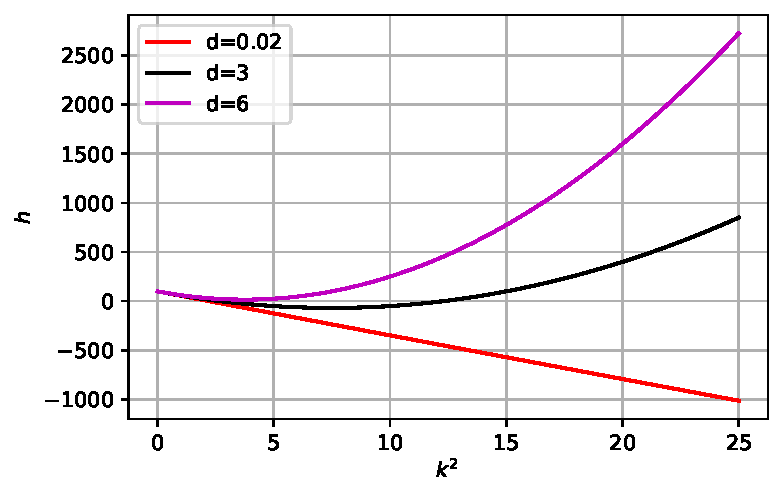
\includegraphics{DiffusionDrivenInstability_files/figure-pdf/fig-dispersion-output-3.pdf}

}

\caption{A plot of \(h(k^2)\) against k\^{}2.}

\end{figure}

\begin{figure}[H]

{\centering 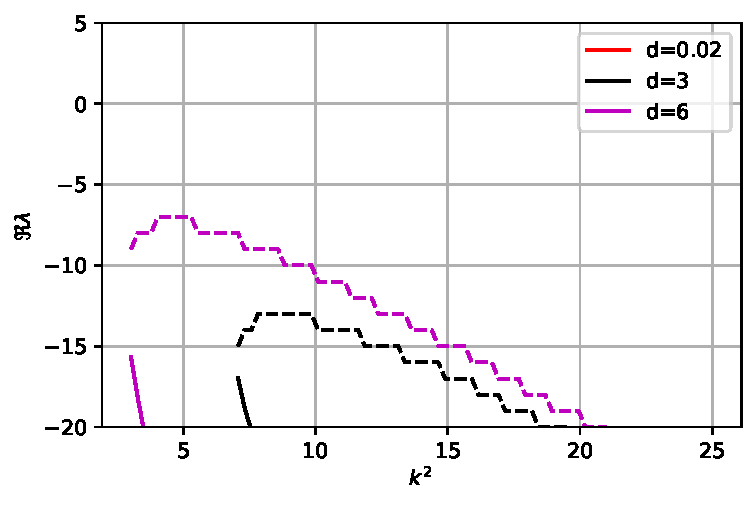
\includegraphics{DiffusionDrivenInstability_files/figure-pdf/fig-dispersion-output-4.pdf}

}

\end{figure}

}

\caption{\label{fig-dispersion}\textbf{?(caption)}}

\end{figure}

\textbf{NOTE}: From Equation~\ref{eq-charact_pp_1},
Equation~\ref{eq-spatial_eigenvalues} we can recover the characteristic
equation for the spatially homogeneous perturbation when \(k=0\), i.e.~
\[
\tilde J \Big|_{k=0} = ( \gamma J - k^2 D )\Big|_{k=0} = \gamma J.
\]

Thus the steady state \((u_0, v_0)\) is \textbf{unstable} to spatially
heterogeneous perturbations iff \[
{\mathrm Re}(\lambda_1) > 0 \quad \text{and/or } \quad {\mathrm Re}(\lambda_2) >0,
\] where \(\lambda_{1,2}\) are solutions of
Equation~\ref{eq-charact_pp_1}, Equation~\ref{eq-spatial_eigenvalues}.

Now for \[
{\mathrm Re}(\lambda_1) > 0 \quad \text{and/or } \quad {\mathrm Re}(\lambda_2) >0
\] to be satisfied we require \[
\text{tr}(\tilde J) > 0 \quad \text{ or } \quad \det(\tilde J) <0 \; .
\]

Consider first \({\mathrm tr} (\tilde{J})\). We have \[
\text{tr}(\tilde J) = \gamma ( f_u+ g_v) - k^2(1+d) < 0, \hspace{4 cm}  
\] since \(\gamma > 0\) and \[ 
f_u+ g_v < 0
\] by the stability condition for the spatially homogeneous perturbation
Equation~\ref{eq-stable_hom}.

Thus instability to the spatially heterogeneous perturbation \textbf{can
only occur} if \[
\det(\tilde J) < 0
\] and so we require: \[
\det(\tilde J) = h(k^2) = dk^4  - \gamma ( d\,  f_u + g_v) k^2 + \gamma^2 \det(J) < 0. 
\] From the spatially homogeneous stability conditions
Equation~\ref{eq-stable_hom} we have \(\det(J) >0\). Thus \(h(k^2)<0\)
is possible only if
\begin{equation}\protect\hypertarget{eq-stabil_cond_nes}{}{
d f_u + g_v >0.
}\label{eq-stabil_cond_nes}\end{equation} However, once again, due to
Equation~\ref{eq-stable_hom}, we have \(f_u+ g_v <0\), and so we can
conclude that \emph{\(d\neq 1\) and \(f_u\) and \(g_v\) must have
opposite signs}.

Condition Equation~\ref{eq-stabil_cond_nes} is \textbf{necessary but not
sufficient} to ensure \(h(k^2) <0\). In order to guarantee that
\(h(k^2) < 0\), the minimum value \(h_{{\mathrm min}}\) must be
negative. Differentiating Equation~\ref{eq-hk2} w.r.t. \(k^2\), we find
that:

\begin{equation}\protect\hypertarget{eq-hmin}{}{
k^2_{m} = \gamma \frac{d f_u + g_v}{2d} \;\; \Rightarrow \;\; h_{{\mathrm min}} = \gamma^2 \left[ | J | - \frac{(df_u + g_v)^2}{4d} \right].
}\label{eq-hmin}\end{equation}

Thus the condition that \(h(k^2) < 0\) for some \(k^2\) is:

\[
\frac{(df_u + g_v)^2}{4d} > |J|.
\]

The transition from stability to instability i.e.~\textbf{bifurcation},
occurs when \(h_{{\mathrm min}} = 0\). From Equation~\ref{eq-hmin}, this
means at bifurcation we have
\begin{equation}\protect\hypertarget{eq-bif}{}{
|J| = \frac{(df_u + g_v)^2}{4d}.
}\label{eq-bif}\end{equation}

For a fixed set of kinetics parameters, this means that we have a
\textbf{critical diffusion coefficient} \(d_c \;(>1)\), which, after
re-arranging Equation~\ref{eq-bif}, is the appropriate root of

\begin{equation}\protect\hypertarget{eq-dcrit}{}{
q(d_c) = d^2_c f_u^2 + 2( 2 f_v g_u - f_u g_v) d_c + g_v^2 =0.
}\label{eq-dcrit}\end{equation}

Finally, we note that using Equation~\ref{eq-hmin},
Equation~\ref{eq-bif}, the \textbf{critical wave number} can be written:
\begin{equation}\protect\hypertarget{eq-kcrit}{}{
k_c^2 =\gamma  \frac{( d_c f_u + g_v)} { 2 d_c} = \gamma \left[ \frac {|J|}{d_c} \right]^{1/2} = \gamma \left[ \frac{f_u g_v - f_v g_u}{d_c} \right]^{1/2}. 
}\label{eq-kcrit}\end{equation}

Figure~\ref{fig-dispersion} (a) shows a schematic diagram of the
(quadratic) function \(h(k^2)\) for three different values of the
diffusion coefficient \(d\):

\begin{itemize}
\tightlist
\item
  \(d < d_c, \; h(k^2) > 0\), and there is no pattern;
\item
  \(d = d_c, \; h_{{\mathrm{min}}} = 0\), critical case;
\item
  \(d > d_c, \; h(k^2) < 0\), and there is pattern.
\end{itemize}

Hence we can see from Equation~\ref{eq-spatial_eigenvalues} that
whenever \(h(k^2) < 0\) the curve \(\lambda(k^2)\) is positive for the
same range of wavenumbers that make \(h(k^2)\) negative. The range of
unstable wavenumbers \[
k^2_1 < k^2 < k^2_2
\] can be found from the roots of Equation~\ref{eq-hk2}, \(h(k^2) = 0\):

\begin{equation}\protect\hypertarget{eq-k2range}{}{
\begin{aligned}
k^2_1 &= \gamma \frac{(df_u + g_v) - \left\{ (df_u + g_v)^2 -4d |J| \right\}^{1/2} }{2d} < k^2  \\
&< \gamma \frac{(df_u + g_v) +  \left\{ (df_u + g_v)^2 -4d |J| \right\}^{1/2}}{2d} = k^2_2 
\end{aligned}
}\label{eq-k2range}\end{equation}

Figure~\ref{fig-dispersion} (b) shows a schematic diagram of
\({\mathrm Re}\lambda (k^2)\) for three different values of the
diffusion coefficient \(d\): * \$d \textless{} d\_c, ;
\({\mathrm Re}\lambda (k^2)\) \textless{} 0, \forall k\^{}2 \$, and
there is no pattern; * \(d = d_c, \; k^2_c = 0\), critical case;

The expression \(\lambda = \lambda (k^2)\) is known as the
\textbf{dispersion relation} and the plot of \({\mathrm Re} \lambda\)
against \(k^2\) is known as the \textbf{dispersion curve}.

From the previous analysis, within the unstable range of wavenumbers
\((k^2_1 , k^2_2)\), \({\mathrm Re}\lambda (k^2) > 0\) has a
\textbf{maximum value} at wavenumber \(k^2_m\) given by
Equation~\ref{eq-hmin} when \(d > d_c\). This implies that there is a
\textbf{fastest growing mode} in the solution Equation~\ref{eq-vxt} of
our linearised system Equation~\ref{eq-pp_4}.

Recalling Equation~\ref{eq-vxt},\\
\[
V(x,t) = \sum_k C_k e^{\lambda(k^2) t} \, \psi_k(x),
\] and noting the above analysis, this implies that as \(t\to \infty\)
the dominant contributions in the above sum are those for which
\({\mathrm Re} \lambda(k^2) > 0\), since all other modes will tend to
zero exponentially fast as \(t\to \infty\). Thus, for large \(t\), the
solution is effectively given by: \[
V(x,t) \approx \sum_{k_{1}}^{k_2} C_k e^{\lambda(k^2) t} \, \psi_k(x) \; .
\]

\%The critical value of \(d=d_c\) at which the bifurcation to
instability occurs is defined by \(h_{\textrm{min}} =0\), i.e.~such
value of \(d\) at which \(h(k^2)=0\) has a double root.

** include figure dispersion **

\textbf{NOTE}

All the previous calculations concern a \textbf{linear stability
analysis} carried out about a spatially homogeneous steady state of the
system Equation~\ref{eq-pp}. This linear theory indicates that for
\(d > d_c\) there exists a finite number of \textbf{linearly unstable}
spatial eigenfunctions which grow exponentially as \(t \to \infty\).
However, this linear theory holds only when we are close to the steady
state i.e.~it only holds for small perturbations. In the full
\textbf{nonlinear system} the exponentially growing (unbounded) modes
will eventually be bounded by the nonlinear terms and so bounded, stable
spatial patterns characterised by the corresponding wavenumbers will be
formed.

\textbf{Summary}

We have obtained conditions for the generation of spatial patterns via
systems of reaction-diffusion equations of the general form
Equation~\ref{eq-pp}. Such systems involve \textbf{two chemicals or
morphogens} reacting and diffusing together to generate a chemical
pre-pattern that underlies a subsequent cellular pattern. The four
conditions are as follows:

\begin{equation}\protect\hypertarget{eq-pattern_conditions}{}{
\begin{aligned}
f_u + g_v &< 0, \\
f_u g_v - f_v g_u &> 0, \\
d f_u + g_v &> 0, \\
(d f_u + g_v)^2 - 4d (f_u g_v - f_v g_u)^2 &< 0 , \nonumber 
\end{aligned}
}\label{eq-pattern_conditions}\end{equation} with all partial
derivatives being evaluated at the spatially homogeneous steady state
\((u_0 , v_0)\).

From the first and third conditions, \(d \neq 1\) and \(f_u\) and
\(g_v\) must be of different signs. For each of the reaction kinetics
mentioned here (Schnakenberg, Gierer-Meinhardt, Thomas), we have that
\(f_u > 0, g_v < 0\) and so this implies that \(d > 1\).

If the conditions Equation~\ref{eq-pattern_conditions} are satisfied,
then there is a range of unstable wavenumbers given by
Equation~\ref{eq-k2range} which give rise to a spatial pattern. The
spatial patterns which initially grow are those spatial eigenfunctions
\(\psi_k(x)\) whose wavenumbers \(k\) are such that \(k_1 < k < k_2\).

In most biological systems, the kinetic parameters and diffusion
coefficients are fixed. This means that the only variable parameter in
the system is \(\gamma\) which as we have seen is related to the size of
the domain under consideration. This has implications when considering
patterns on finite domains, as will be seen in the next section.

\hypertarget{exercises}{%
\section{Exercises}\label{exercises}}

Demonstrate that the derived results are consistent with numerical
solutions. Some predictions to test:

\begin{itemize}
\tightlist
\item
  No patterning when diffusion coefficients are equal
\item
  How does spatial pattern formation change as you try values of
  parameters \(a\) and \(b\)?
\item
  Can you correlate the observation of pattern to the conditions for DDI
  being satisfied?
\item
  what about different kinetics (e.g.~Gierer-Meinhardt, Thomas models)?
\end{itemize}

\hypertarget{references-1}{%
\section{References}\label{references-1}}

\hypertarget{mathematical-modelling-of-infectious-disease}{%
\chapter{Mathematical modelling of infectious
disease}\label{mathematical-modelling-of-infectious-disease}}

Mathematical modelling of infection diseases can help to understand
complex (nonlinear) interactions, to design vaccination strategies,
predict further outbreaks of diseases, how many individual will be
affected.

Assumptions * Total population is constant: the duration of the epidemic
is short compared to the lifetime of its hosts, so we can neglect birth
and disease-unrelated death

*Consider a disease which, after recovery, confers immunity (and/or
death if lethal)

\begin{itemize}
\tightlist
\item
  Simple diffusion for spatial distribution of population
\end{itemize}

Consider consider three classes of population density * \(S\) --
susceptibles - such that can be infected * \(I\) -- invectives - such
that have the disease and can transmit it to susceptibles * \(R\) --
recovered (removed) - such that have had the disease and are immune or
isolate until recovered or death (if the disease is lethal)

Progress through the disease \[
S \longrightarrow I \longrightarrow R 
\]

Model assumptions * The gain in the invectives class is at the rate
proportional to the number of invectives \(I\) and susceptibles \(S\),
i.e.~\(r\; I\; S\), ; \(r>0\).

\begin{itemize}
\tightlist
\item
  The susceptibles are lost at the same rate, i.r. \(r\; I\; S\)

  \item

  The rate of removal of invectives to the recovered class \(R\) is
  proportional to the number of invectives, i.e.~\(a\; I\), ; \(a>0\).
\end{itemize}

\$ 1/a \$ measures the time spent in the infectious state.

\begin{itemize}
\tightlist
\item
  The incubation period is short enough to be negligible: susceptibles
  are directly infected after coming into contact with the disease (with
  invectives).
\end{itemize}

Then a simple SIR model reads (in a long thin domain or in \(3\)-dim
domain with solutions in a form of planar fronts) \[
\begin{aligned}
&\frac{\partial S}{\partial t} = - r SI + D_S \frac{ \partial^2 S}{\partial x^2}\; ,  &\qquad x \in \mathbb R , \; t>0 \; , \\
&\frac{\partial I}{\partial t} = r SI - a I+ D_I \frac{ \partial^2 I}{\partial x^2} \; ,  &\qquad x \in \mathbb R , \; t>0 \; , \\
&\frac{\partial R}{\partial t} = a I + D_R \frac{ \partial^2 R}{\partial x^2} \; , & \qquad x \in \mathbb R , \; t>0 \; \\
&S(0,x) = S_0(x), \qquad I(0,x) = I_0(x), \quad R(0,x) = R_0(x),& \qquad x \in \mathbb R \; , 
\end{aligned}
\]

where * \(a>0\) -- removal or death rate * \(r>0\) -- transmission or
infection rate * \(D_S>0\), ; \(D_I>0\), ; \(D_R>0\) -- diffusion
coefficients

We assume that \(S_0(x) \geq 0\), \(I_0(x) \geq 0\), \(R_0(x) \geq 0\)
for \(x \in \mathbb R\) and obtain that solutions of \eqref{SIR1} are
nonnegative, i.e.~ \[
S(t,x) \geq 0, \quad I(t,x) \geq 0, \quad R(t,x) \geq 0, \quad  x\in \mathbb R, \quad t >0 \; .
\]

To analyse the model \eqref{SIR1} it is sufficient to consider the first
two equations, since \(R\) is completely determined by \(I\) and does
not influence the dynamics of \(S\) and \(I\).

Considering the non-dimensionalisation \[
I^\ast = \frac I{\bar S_0} , \quad S^\ast = \frac S{\bar S_0} ,  \quad x^\ast = \left(\frac{ r \bar S_0}{D_I} \right)^{1/2} x, \quad t^\ast = r \bar S_0 t 
\] we obtain ( after dropping \(`\ast'\))

\[
\begin{aligned}
& \frac{\partial S}{\partial t} = -  SI + d \frac{ \partial^2 S}{\partial x^2}\; , & \qquad x \in \mathbb R , \; t>0 \; , \\
& \frac{\partial I}{\partial t} = SI - \mu I+  \frac{ \partial^2 I}{\partial x^2} \; ,  & \qquad x \in \mathbb R , \; t>0 \; , \\
& S(0,x) = \frac{S_0(x)}{\bar S_0}, \qquad I(0,x) = \frac{I_0(x)}{\bar S_0},  & \quad x \in \mathbb R \; ,
\end{aligned}
\] where \(\bar S_0\) is a representative population density and
\(\mu = a /{ r \bar S_0}\).

We would like to investigate the spatial spread of an epidemic wave of
invectives into a uniform susceptibles population \(S_0(x) =\bar S_0\).
We would like to determine conditions for existence of an epidemic wave
and propagation speed.

We shall assume first that \(D_S= D_I\), i.e.~\(d=1\). Consider
travelling wave solutions \[
S(t,x) = s(z), \quad I(t,x) = i(z), \quad z = x - v t, \quad v >0
\] and obtain following ODEs for \(s\) and \(i\)
\begin{equation}\protect\hypertarget{eq-sit_tw}{}{
\begin{aligned}
s^{\prime \prime} + v s^\prime - i s = 0 \; , \\
i^{\prime \prime} + v i^\prime + i s - \mu i= 0\; .
\end{aligned}
}\label{eq-sit_tw}\end{equation}

We would like to analyse the existence of a travelling wave from for
\(S\) and travelling wave pulse for \(I\). We assume that the infection
comes into susceptible population from the left.

Therefore we consider the following boundary conditions for the
travelling wave solutions

\begin{equation}\protect\hypertarget{eq-sir_tw_bx}{}{
\begin{aligned}
s(z) \to 1 \qquad  z\to + \infty, \quad \qquad  i(z) \to 0 \qquad  z\to + \infty\; ,\\
s(z) \to \sigma \qquad  z\to - \infty, \quad \qquad  i(z) \to 0 \qquad  z\to - \infty\; ,\\
s^\prime(z) \to 0\qquad  z\to \pm \infty, \quad \qquad i^\prime(z) \to 0 \qquad z \to \pm \infty \; ,
\end{aligned}
}\label{eq-sir_tw_bx}\end{equation} where \(0 \leq \sigma <1\).

The steady states of Equation~\ref{eq-sit_tw} are given by \[
 is =0 , \quad i ( s- \mu) = 0  \quad \Longrightarrow \quad \ i=0, \quad s = \text{const} \; .
\] Considering boundary conditions \textbf{?@eq-sir\_tw\_bc} we obtain
two steady states \[
(s_0, i_0) = ( 1, 0), \qquad (s_0, i_0) = (\sigma, 0)
\] Hence we would like to have a heteroclinic connection between
\((\sigma , 0)\) and \((1,0)\).

The necessary condition for existence of travelling wave solutions
satisfying (\textbf{sir\_tw?}) and \textbf{?@eq-sir\_tw\_bc} is

\begin{equation}\protect\hypertarget{eq-cond_v_sir}{}{
 v \geq 2 \sqrt{ 1- \mu} \, \quad \text{ and } \quad 0 \leq \mu < 1\; .  
}\label{eq-cond_v_sir}\end{equation}

In terms of original parameters we have \[
 \mu = \frac a { r S_0} < 1. 
 \] This is the necessary threshold conditions for the propagation of an
epidemic wave pulse. The condition \eqref{cond_v_SIR} determine also the
non-dimensionalised minimal wave speed \[
v^\ast_{\text{min}} = 2\sqrt{ 1- \mu}
\]

In dimensional terms we obtain \[
z^\ast = x^\ast - v^\ast t^\ast = \left( \frac { r S_0} {D_I} \right)^{1/} x - v^\ast r S_0 t  = 
\left( \frac { r S_0} {D_I} \right)^{1/} ( x - v t) = \left( \frac { r S_0} {D_I} \right)^{1/} z
\] and \[
v = \sqrt{ r S_0 D_I} v^\ast \quad v_{\text{min}} = 2  \sqrt{ r S_0 D_I}\sqrt{ 1- \mu} = 
2  \sqrt{ r S_0 D_I}\sqrt{ 1- \frac a{ r S_0} }
\]

We can analyse the behaviour of travelling wave solutions as
\(z \to + \infty\).

Linearised equation for the second equation in \textbf{?@eq-sir\_tw}
near \(s=1\), \(i=0\), i.e.~as \(z \to + \infty\) reads \[
i^{\prime \prime} + v i^\prime + i  - \mu i = 0\; .
\] Thus

\begin{equation}\protect\hypertarget{eq-i_tw_infty}{}{
i(z) \sim \exp \left(\frac 1 2 \left[ - v \pm \sqrt{ v^2 - 4(1-\mu)} \right] z \right) \quad \text{ as } z \to + \infty \; . 
}\label{eq-i_tw_infty}\end{equation} We can also show that the
travelling wave solution \(s(z)\) can not have a local maximum, since
for \(s^\prime(z) = 0\) first equation in \textbf{?@eq-sir\_tw} implies
\[
s^{\prime \prime}(z) = is >0, 
\] which implies a local minimum. So \(s(z)\) is monotone increasing.

Considering linearisation of the first equation in \textbf{?@eq-sir\_tw}
near \(s=1\), \(i=0\), i.e.~as \(z \to + \infty\), we obtain with
\(s(z) = 1 - \tilde s(z)\) \[
\tilde s^{\prime \prime} + v \tilde s^{\prime} - i = 0 \; . 
\] The using Equation~\ref{eq-i_tw_infty} we can conclude that

\begin{equation}\protect\hypertarget{eq-tilde_s_tw_infty}{}{
\tilde s(z) \sim \exp \left(\frac 1 2 \left[ - v \pm \sqrt{ v^2 - 4(1-\mu)} \right] z \right) \quad \text{ as } z \to + \infty \; . 
}\label{eq-tilde_s_tw_infty}\end{equation} and

\begin{equation}\protect\hypertarget{eq-s_tw_infty}{}{
 s(z) \sim 1 - C \exp \left(\frac 1 2 \left[ - v \pm \sqrt{ v^2 - 4(1-\mu)} \right] z \right) \quad \text{ as } z \to + \infty \; . 
}\label{eq-s_tw_infty}\end{equation}

\hypertarget{spatial-spread-of-rabies-among-foxes}{%
\section{Spatial spread of rabies among
foxes}\label{spatial-spread-of-rabies-among-foxes}}

Spread of rabies is due primary to the migration of infected foxes. We
assume the heathy foxes are territorial and do not travel very far,
whereas rabid foxes wander over large distances.

Thus we assume that \(D_S \ll D_I\) and \(d= { D_S}/{D_I} \approx 0\).\\
\begin{equation}\protect\hypertarget{eq-sir3}{}{
\begin{aligned}
& \frac{\partial S}{\partial t} = -  SI \; , & \qquad x \in \mathbb R , \; t>0 \; , \\
& \frac{\partial I}{\partial t} = SI - \mu I+  \frac{ \partial^2 I}{\partial x^2} \; ,  & \qquad x \in \mathbb R , \; t>0 \; , \\
& S(0,x) = 1, \qquad I(0,x) = \frac{I_0}{\bar S_0},  & \quad x \in \mathbb R \; ,
\end{aligned}
}\label{eq-sir3}\end{equation}

We shall look for travelling wave solutions of \eqref{SIR3}: travelling
wave front for \(S\) and travelling wave pulse for \(I\). Considering \[
S(t,x) = s(z), \quad I(t,x) = i(z), \quad z = x - v t, \quad v >0
\] and obtain following ODEs for \(s\) and \(i\)

\begin{equation}\protect\hypertarget{eq-sir_tw_2}{}{
\begin{aligned}
&  v s^\prime = i s  \; , \\
& i^{\prime \prime} + v i^\prime + i s - \mu i= 0\; 
\end{aligned}
}\label{eq-sir_tw_2}\end{equation} and corresponding boundary conditions

\begin{equation}\protect\hypertarget{eq-sir_tw_bc_2}{}{
\begin{aligned}
s(z) \to 1 \qquad  z\to + \infty, \quad \qquad  i(z) \to 0 \qquad  z\to + \infty\; ,\\
s(z) \to \sigma \qquad  z\to - \infty, \quad \qquad  i(z) \to 0 \qquad  z\to - \infty\; ,\\
s^\prime(z) \to 0\qquad  z\to \pm \infty, \quad \qquad i^\prime(z) \to 0 \qquad z \to \pm \infty \; ,
\end{aligned}
}\label{eq-sir_tw_bc_2}\end{equation} where \(0 \leq \sigma <1\).

As before, the steady states of Equation~\ref{eq-sir_tw_2} are given by
\[
 is =0 , \quad i ( s- \mu) = 0  \quad \Longrightarrow \quad  i=0, \quad s = \text{const} \; .
 \] Considering boundary conditions Equation~\ref{eq-sir_tw_bc_2} we
obtain two steady states \[
(s_0, i_0) = ( 1, 0), \qquad (s_0, i_0) = (\sigma, 0) \; .
\]

Linearising equations Equation~\ref{eq-sir_tw_2} about the steady state
\((1,0)\) and requiring that \(i\) is nonnegative we obtain, as for
\textbf{?@eq-sir\_tw}, the necessary conditions for existence of
travelling wave solutions satisfying Equation~\ref{eq-sir_tw_2} and
(\textbf{sir\_tw\_bc\_2?}) : \[
 v \geq 2 \sqrt{ 1- \mu} \, \quad \text{ and } \quad 0 \leq \mu < 1\; .  
\]

We can determine the relation between density of susceptibles left
behind the infection pulse and the model parameters.

Using first equation in Equation~\ref{eq-sir_tw_2} in the second implies
\begin{equation}\protect\hypertarget{eq-sigma_1}{}{
 i^{\prime \prime} + v i^\prime + v s^\prime  - \mu i= 0\; .
}\label{eq-sigma_1}\end{equation} Integrating with respect to \(z\)
yields

\begin{equation}\protect\hypertarget{eq-sigma_2}{}{
 i^{\prime } + v i + v s  - \mu \int i\, dz = K= const\; .
}\label{eq-sigma_2}\end{equation} Consider now ageing the first equation
in Equation~\ref{eq-sir_tw_2} \[
i= v \frac {s^\prime} s, \quad \quad s \neq 0 \; 
\] and obtain from Equation~\ref{eq-sigma_2} \[
 i^{\prime } + v i + v s  - v  \mu \int   \frac {s^\prime} s\, dz = K= const\; .
\] or \begin{equation}\protect\hypertarget{eq-sigma_3}{}{
 i^{\prime } + v i + v s  - v  \mu \ln(s) = K\; .
}\label{eq-sigma_3}\end{equation} Using now in Equation~\ref{eq-sigma_3}
boundary conditions as \(z \to + \infty\), from
Equation~\ref{eq-sir_tw_bc_2}, we can determine constant \(K\):

\[
 v    = K\; .
\] Thus we have \begin{equation}\protect\hypertarget{eq-sigma_4}{}{
 i^{\prime } + v i + v( s  - \mu \ln(s) -1)= 0\; .
}\label{eq-sigma_4}\end{equation} Using now in Equation~\ref{eq-sigma_4}
boundary conditions as \(z \to - \infty\), see
Equation~\ref{eq-sir_tw_bc_2}, gives

\[
 v( \sigma - \mu \ln(\sigma) -1)= 0\; .
\] and \begin{equation}\protect\hypertarget{eq-sigma_5}{}{
\frac{ \sigma- 1}{\ln(\sigma)} = \mu \; . 
}\label{eq-sigma_5}\end{equation} We obtain that the number of
susceptibles is defined independently of the wave speed and the smaller
\(\mu\) corresponds to smaller \(\sigma\) ( i.e.~fever susceptibles
survive infection wave). Thus \(\mu\) measures how sever the epidemic
is.

Considering the critical value for \(\mu =1\), which in dimensional
terms means \[
\frac a { r S_0} = 1, 
\] we can conclude that there exists no wave of infection * if \(S_0\)
is too low - density of foxes is too low in order to spread the
disease,\\
* or if removal rate is too large - high death rate and the infection is
too virulent * or if infection rate \(r\) is too small - the disease is
too

\hypertarget{generalisation-of-simple-sir-model}{%
\subsection{Generalisation of simple SIR
model}\label{generalisation-of-simple-sir-model}}

We developed a simple model for the passage of a wave of infection,
however data of a spread of rabies in continental Europe looks quite
different, i.e.~comprises oscillations behind the wave front. It is
likely that birth-death processes, not included in the simple model,
impact dynamics of susceptibles and invectives.

We generalised the simple model by considering growth of susceptibles
population in a logistic manner

\begin{equation}\protect\hypertarget{eq-sir_growth}{}{
\begin{aligned}
& \frac{\partial S}{\partial t} = -  rSI + B S\left( 1 - \frac S{S_0} \right) \; , & \qquad x \in \mathbb R , \; t>0 \; , \\
& \frac{\partial I}{\partial t} =  r SI - a I+  D_I \frac{ \partial^2 I}{\partial x^2} \; ,  & \qquad x \in \mathbb R , \; t>0 \; , \\
& S(0,x) = S_0, \qquad I(0,x) = I_0,  & \quad x \in \mathbb R \; ,
\end{aligned}
}\label{eq-sir_growth}\end{equation} where \(B\) is the intrinsic growth
rate and \(S_0\) is the carrying capacity.

We can non-dimensionalize Equation~\ref{eq-sir_growth} as before and
obtain \begin{equation}\protect\hypertarget{eq-sir_growth_nd}{}{
\begin{aligned}
& \frac{\partial S}{\partial t} = -  SI + b S\left( 1 -  S \right) \; , & \qquad x \in \mathbb R , \; t>0 \; , \\
& \frac{\partial I}{\partial t} =   SI - \mu \,  I+   \frac{ \partial^2 I}{\partial x^2} \; ,  & \qquad x \in \mathbb R , \; t>0 \; , \\
& S(0,x) = 1, \qquad I(0,x) = I_0/S_0,  & \quad x \in \mathbb R \; ,
\end{aligned}
}\label{eq-sir_growth_nd}\end{equation} where \[
b= \frac{B}{r S_0}.
\]

Spatially homogeneous steady states of Equation~\ref{eq-sir_growth_nd}
are \((S^\ast_1, I^\ast_1) = (1,0)\) and
\((S^\ast_1, I^\ast_1) = (\mu, b(1-\mu))\).

To analyse the existence of travelling wave solutions we write equations
for \(s(z)\) and \(i(z)\), where \(s(z)=S(t,x)\), \(i(z) = I(t,x)\) with
\(z= x- vt\)

\[
\begin{aligned}
&  -v s^\prime =- i s  + b s ( 1-s) \; , \\
& - v i^\prime =  i s - \mu i +  i^{\prime \prime}  \; 
\end{aligned}
\] \{eq-sir\_tw\_growth\} and by introducing new variable
\(w= i^\prime\) obtain

\begin{equation}\protect\hypertarget{eq-sir_tw_growth_2}{}{
 \begin{aligned}
&   s^\prime = \frac 1 v i\,  s  - \frac  b v \,  s ( 1-s) \; , \\
& i^\prime = w, \\
& w^{\prime}= -  v w - i (s - \mu)\; .
\end{aligned}
}\label{eq-sir_tw_growth_2}\end{equation} The system
Equation~\ref{eq-sir_tw_growth_2} has two stationary solutions

\[
(s^\ast_1, i^\ast_1, w^\ast_1) = (1,0,0)
\] and

\[(s^\ast_2, i^\ast_2, w^\ast_2) = (\mu, b(1-\mu),0)
\]. Considering linearisation of Equation~\ref{eq-sir_tw_growth_2} and
computing eigenvalues of the Jabocian matrix \[
J(s,i,w)= \begin{pmatrix}
\frac{i}{v} - \frac{b}{v}  + \frac{2bs}{v} & \frac{s}{v} & 0 \\
0 & 0 & 1\\
- i & \mu - s & -v
\end{pmatrix}
\]

evaluated at the steady states we obtain that \[
 (s^\ast_1, i^\ast_1, w^\ast_1) = (1,0,0)
\]

is a saddle point and \[
 (s^\ast_2, i^\ast_2, w^\ast_2) = (\mu, b(1-\mu),0)
\]

is a stable node for \(\mu < \mu^\ast\) and a stable spiral (focus) for
\(\mu >\mu^\ast\), with some threshold value \(\mu^\ast\).

Thus we can show that a travelling wave solution exists which connects
two steady states \((1,0)\) and \((\mu, b(1-\mu))\) and there exists a
threshold \(\mu = \mu^\ast\) such that for
\$1\textgreater{}\mu \textgreater{} \mu\^{}\ast \$ the approach to
\((\mu, b(1-\mu))\) is oscillatory, whereas for \(0<\mu < \mu^\ast\) it
is monotonic.

\part{Appendices}

\hypertarget{numerical-methods-in-python}{%
\chapter{Numerical methods in
Python}\label{numerical-methods-in-python}}

\hypertarget{python-libraries}{%
\section{Python libraries}\label{python-libraries}}

\begin{itemize}
\tightlist
\item
  matplotlib
\item
  numpp
\item
  scipy
\end{itemize}

\hypertarget{single-pdes}{%
\section{Single PDEs}\label{single-pdes}}

\hypertarget{mol}{%
\subsection{MOL}\label{mol}}

\hypertarget{spatial-discretisation}{%
\subsection{Spatial discretisation}\label{spatial-discretisation}}

\hypertarget{odeint}{%
\subsection{odeint}\label{odeint}}

\hypertarget{implementing-boundary-conditions}{%
\subsection{implementing boundary
conditions}\label{implementing-boundary-conditions}}

\hypertarget{identifying-parameters}{%
\subsection{Identifying parameters}\label{identifying-parameters}}

\hypertarget{systems-of-pdes}{%
\section{Systems of PDEs}\label{systems-of-pdes}}

\hypertarget{linear-stability-analysis-of-a-system-of-nonlinear-odes}{%
\chapter{Linear stability analysis of a system of nonlinear
ODES}\label{linear-stability-analysis-of-a-system-of-nonlinear-odes}}

Consider a system of ODEs

\begin{equation*}
\frac{du}{dt} = f(u) \quad \text{ with } \quad u \in \mathbb R^m\quad  \text{ and }\quad  t \in \mathbb R. 
\end{equation*}

As an example consider \(m=2\):
\begin{equation}\protect\hypertarget{eq-system_ode11}{}{
\begin{aligned}
\begin{cases}
\dfrac{du_1}{dt} =F(u_1, u_2) ,\\
\dfrac{du_2}{dt} =G(u_1, u_2)
\end{cases}
\end{aligned}
}\label{eq-system_ode11}\end{equation}

\((u_1, u_2) = (u^\ast_1, u^\ast_2)\) is the steady state of the system
Equation~\ref{eq-system_ode11}, i.e. \[ 
\dfrac{du_1}{dt} = 0
\] and \[ 
 \dfrac{du_2}{dt} = 0 
 \].

To determine the behaviour of the solution near a steady state we
consider \[
u_1(t) = u^\ast_1 + \bar u_1(t), \quad  u_2(t) = u^\ast_2 + \bar u_2(t)
\] \begin{equation}\protect\hypertarget{eq-system_ode12}{}{
\begin{aligned}
\begin{cases}
\dfrac{d(u^\ast_1+ \bar u_1)}{dt} =F(u^\ast_1+ u_1, u^\ast_2+ \bar u_2) ,\\
\dfrac{d(u^\ast_2+\bar u_2)}{dt} =G(u^\ast_1+u_1,u^\ast_2+\bar u_2)
\end{cases}
\end{aligned}
}\label{eq-system_ode12}\end{equation}

Then using the fact that \((u^\ast_1, u^\ast_2)\) is a steady state and
applying Taylor series expansion about \(( u^\ast_1, u^\ast_2)\) and
assuming that\\
\[
\sup_{t}|\bar u_1(t)| \ll 1, \sup_{t}|\bar u_2(t)|\ll 1
\] (small perturbations of the steady state) we have
\begin{equation}\protect\hypertarget{eq-system_ode13}{}{
\begin{aligned}
\begin{cases}
\dfrac{d  \bar u_1}{dt} =F(u^\ast_1, u^\ast_2) +\dfrac{\partial F}{\partial u_1}(u^\ast_1, u^\ast_2) \,   \bar u_1
+\dfrac{\partial F}{\partial u_2}(u^\ast_1, u^\ast_2) \, \bar u_2 + O(|\bar u_1|^2, |\bar u_2|^2) ,\\
\dfrac{d \bar u_2}{dt} =G(u^\ast_1,u^\ast_2)+ \dfrac{\partial G}{\partial u_1}(u^\ast_1, u^\ast_2) \,   \bar u_1
+\dfrac{\partial G}{\partial u_2}(u^\ast_1, u^\ast_2) \,\bar u_2 + O(|\bar u_1|^2, |\bar u_2|^2) 
\end{cases}
\end{aligned}
}\label{eq-system_ode13}\end{equation}

Thus since \((u^\ast_1, u^\ast_2)\) is a steady state,
i.e.~\(F(u^\ast_1, u^\ast_2) =0\) and \(G(u^\ast_1, u^\ast_2) =0\)
(ignoring negligibly small higher order terms) we obtain system of
linearised equations
\begin{equation}\protect\hypertarget{eq-system_ode14}{}{
\begin{aligned}
\begin{pmatrix}
\dfrac{d  \bar u_1}{dt} \\
\dfrac{d \bar u_2}{dt} 
\end{pmatrix} = J( u^\ast_1, u^\ast_2) \begin{pmatrix} \bar u_1 \\
\bar u_2 
\end{pmatrix}
\end{aligned}
}\label{eq-system_ode14}\end{equation} where the Jacobian matrix
\(J(u^\ast_1, u^\ast_2)\) is defined as \[
J( u^\ast_1, u^\ast_2) = \begin{pmatrix}
\dfrac{\partial F(u^\ast_1, u^\ast_2) }{\partial u_1}\; \; & \dfrac{\partial F(u^\ast_1, u^\ast_2)}{\partial u_2}\\
\dfrac{\partial G(u^\ast_1, u^\ast_2)}{\partial u_1} & \dfrac{\partial G(u^\ast_1, u^\ast_2)}{\partial u_2}
\end{pmatrix}
\] Therefore the behaviour of the nonlinear system
Equation~\ref{eq-system_ode11} near the steady state
\((u^\ast_1, u^\ast_2)\) is determined by solutions of system of linear
ODEs Equation~\ref{eq-system_ode14}.

Since Equation~\ref{eq-system_ode14} is linear we can write the general
solution of (\textbf{eqsystem\_ode14?}) \begin{equation}
\begin{pmatrix} \bar u_1 \\
\bar u_2 
\end{pmatrix} = e^{\lambda_1 t} \begin{pmatrix} \phi_1 \\
\phi_2 
\end{pmatrix}   +
e^{\lambda_2 t} \begin{pmatrix} \psi_1 \\
\psi_2 
\end{pmatrix}
\end{equation} where \(\lambda_1\) and \(\lambda_2\) are eigenvalues of
Jacobian matrix \(J( u^\ast_1, u^\ast_2)\) and \[
\phi=\begin{pmatrix} \phi_1 \\
\phi_2 
\end{pmatrix} \quad \textrm{and} \quad  \psi= \begin{pmatrix} \psi_1 \\
\psi_2 
\end{pmatrix}
\] are corresponding eigenvectors.

Denote \[\bar u=
\begin{pmatrix} \bar u_1 \\
\bar u_2 
\end{pmatrix}
\].

If both \(\lambda_{1,2} \neq 0\) then the stability of the steady state
\((u^\ast_1, u^\ast_2)\) is determined by the real part of the
eigenvalues \(\lambda_{1,2}\).

\begin{itemize}
\item
  If either \(\mathcal Re (\lambda_1)>0\) or
  \(\mathcal Re (\lambda_2)>0\) then\\
  \(|\bar u(t)| \to +\infty\) as \(t \to + \infty\) and
  \((u^\ast_1, u^\ast_2)\) is unstable.
\item
  If \(\mathcal Re (\lambda_1)<0\) and \(\mathcal Re (\lambda_2)<0\)
  then\\
  \(|\bar u(t)| \to 0\) as \(t \to + \infty\) and
  \((u^\ast_1, u^\ast_2)\) is stable.
\item
  If \(\lambda_1=0\) or \(\lambda_2=0\) we have to consider higher order
  terms.
\end{itemize}

Denote \(\beta = \textrm{tr} (J( u^\ast_1, u^\ast_2))\) and
\(\gamma= \det(J( u^\ast_1, u^\ast_2))\). Then the characteristic
(eigenvalue) equation for \(J( u^\ast_1, u^\ast_2)\) is \[
\lambda^2 - \beta \lambda + \gamma = 0 \; , \quad  \lambda_{1,2} = \frac{ \beta \pm \sqrt{ \beta^2 - 4 \gamma}} 2.
\] Then

\begin{itemize}
\item
  If \(\gamma <0\) we have two real eigenvalues with different signs,
  i.e.~\(\lambda_1 < 0 < \lambda_2\). Thus \((u^\ast_1, u^\ast_2)\) is a
  \textbf{saddle}.
\item
  If \(\gamma >0\) and \(\beta^2 \geq 4\gamma\) we have two real
  eigenvalues with the same sign. Thus \((u^\ast_1, u^\ast_2)\) is a
  \textbf{node}.

  \begin{itemize}
  \tightlist
  \item
    if \(\beta >0\) then \(\lambda_2 > \lambda_1 >0\) and
    \((u^\ast_1, u^\ast_2)\) is an \textbf{unstable node}.
  \item
    if \(\beta <0\) then \(\lambda_1 < \lambda_2 < 0\) and
    \((u^\ast_1, u^\ast_2)\) is a \textbf{stable node}.
  \end{itemize}
\item
  If \(\gamma >0\) and \(\beta^2 < 4\gamma\) we have two complex
  conjugate eigenvalues. Thus \((u^\ast_1, u^\ast_2)\) is a
  \textbf{focus (spiral)}.

  \begin{itemize}
  \item
    if \(\beta >0\) then \(\mathcal Re(\lambda_{1,2}) > 0\) and
    \((u^\ast_1, u^\ast_2)\) is an \textbf{unstable focus}
  \item
    if \(\beta <0\) then \(\mathcal Re(\lambda_{1,2}) < 0\) and
    \((u^\ast_1, u^\ast_2)\) is a \textbf{stable focus}.
  \item
    If \(\beta =0\) then for linear system we have a \textbf{centre},
    but in general we have no information on the behaviour of the
    nonlinear system near the steady state \((u^\ast_1, u^\ast_2)\).
  \end{itemize}
\end{itemize}

** Insert figure phase plane **

\hypertarget{refs}{}
\begin{CSLReferences}{1}{0}
\leavevmode\vadjust pre{\hypertarget{ref-gierer1972theory}{}}%
{``A Theory of Biological Pattern Formation.''} 1972. \emph{Kybernetik}
12: 30--39.

\leavevmode\vadjust pre{\hypertarget{ref-durston2013dictyostelium}{}}%
Durston, AJ. 2013. {``Dictyostelium: The Mathematician's Organism.''}
\emph{Current Genomics} 14 (6): 355--60.

\leavevmode\vadjust pre{\hypertarget{ref-kolmogorov1937investigation}{}}%
Kolmogorov, AN, IG Petrovsky, and NS Piskunov. 1937. {``Investigation of
the Equation of Diffusion Combined with Increasing of the Substance and
Its Application to a Biology Problem.''} \emph{Bull. Moscow State Univ.
Ser. A: Math. Mech} 1 (6): 1--25.

\leavevmode\vadjust pre{\hypertarget{ref-murray2003mathematical}{}}%
Murray, James Dickson. 2003. \emph{Mathematical Biology: II: Spatial
Models and Biomedical Applications}. Vol. 3. Springer.

\leavevmode\vadjust pre{\hypertarget{ref-murray1984generation}{}}%
Murray, James D, and George F Oster. 1984. {``Generation of Biological
Pattern and Form.''} \emph{Mathematical Medicine and Biology: A Journal
of the IMA} 1 (1): 51--75.

\leavevmode\vadjust pre{\hypertarget{ref-murray1981pre}{}}%
Murray, JD610574. 1981. {``A Pre-Pattern Formation Mechanism for Animal
Coat Markings.''} \emph{Journal of Theoretical Biology} 88 (1): 161--99.

\leavevmode\vadjust pre{\hypertarget{ref-fisher1937wave}{}}%
{``The Wave of Advance of Advantageous Genes.''} 1937. \emph{Annals of
Eugenics} 7 (4): 355--69.

\leavevmode\vadjust pre{\hypertarget{ref-turing1990chemical}{}}%
Turing, Alan Mathison. 1990. {``The Chemical Basis of Morphogenesis.''}
\emph{Bulletin of Mathematical Biology} 52: 153--97.

\end{CSLReferences}



\end{document}
